% Options for packages loaded elsewhere
\PassOptionsToPackage{unicode}{hyperref}
\PassOptionsToPackage{hyphens}{url}
\documentclass[
  indonesian,
  11pt,
  a4paper,
  oneside,
  openany]{report}
\usepackage{xcolor}
\usepackage{amsmath,amssymb}
\setcounter{secnumdepth}{-\maxdimen} % remove section numbering
\usepackage{iftex}
\ifPDFTeX
  \usepackage[T1]{fontenc}
  \usepackage[utf8]{inputenc}
  \usepackage{textcomp} % provide euro and other symbols
\else % if luatex or xetex
  \usepackage{unicode-math} % this also loads fontspec
  \defaultfontfeatures{Scale=MatchLowercase}
  \defaultfontfeatures[\rmfamily]{Ligatures=TeX,Scale=1}
\fi
\usepackage{lmodern}
\ifPDFTeX\else
  % xetex/luatex font selection
  \setmainfont[]{Charter}
  \setsansfont[]{Arial}
  \setmonofont[]{Menlo}
\fi
% Use upquote if available, for straight quotes in verbatim environments
\IfFileExists{upquote.sty}{\usepackage{upquote}}{}
\IfFileExists{microtype.sty}{% use microtype if available
  \usepackage[]{microtype}
  \UseMicrotypeSet[protrusion]{basicmath} % disable protrusion for tt fonts
}{}
\makeatletter
\@ifundefined{KOMAClassName}{% if non-KOMA class
  \IfFileExists{parskip.sty}{%
    \usepackage{parskip}
  }{% else
    \setlength{\parindent}{0pt}
    \setlength{\parskip}{6pt plus 2pt minus 1pt}}
}{% if KOMA class
  \KOMAoptions{parskip=half}}
\makeatother
\usepackage{longtable,booktabs,array}
\usepackage{caption}
\captionsetup[table]{skip=6pt}
\newcounter{none} % for unnumbered tables
\usepackage{calc} % for calculating minipage widths
% Correct order of tables after \paragraph or \subparagraph
\usepackage{etoolbox}
\makeatletter
\patchcmd\longtable{\par}{\if@noskipsec\mbox{}\fi\par}{}{}
\makeatother
% Allow footnotes in longtable head/foot
\IfFileExists{footnotehyper.sty}{\usepackage{footnotehyper}}{\usepackage{footnote}}
\makesavenoteenv{longtable}
\ifLuaTeX
\usepackage[bidi=basic,shorthands=off,provide=*]{babel}
\else
\usepackage[bidi=default,shorthands=off,provide=*]{babel}
\fi
\ifPDFTeX
\else
\babelfont{rm}[]{Charter}
\fi
\ifLuaTeX
  \usepackage{selnolig} % disable illegal ligatures
\fi
\setlength{\emergencystretch}{3em} % prevent overfull lines
\providecommand{\tightlist}{%
  \setlength{\itemsep}{0pt}\setlength{\parskip}{0pt}}
% Print-oriented additions for the combined Chapter 2 packet.
\usepackage[a4paper,top=25mm,bottom=25mm,left=30mm,right=25mm,headheight=16pt,headsep=7mm,footskip=12mm]{geometry}
\usepackage{microtype}
\usepackage{setspace}
\usepackage{ragged2e}
\usepackage{fancyhdr}
\usepackage{titlesec}
\usepackage{enumitem}
\usepackage{needspace}
\usepackage{etoolbox}
\usepackage{array}
\usepackage{booktabs}
\usepackage{longtable}
\usepackage{tabularx}
\usepackage{adjustbox}
\usepackage{float}
\usepackage{pdfpages}
\usepackage{tikz}
\usetikzlibrary{arrows.meta,positioning,calc}
\usepackage[most]{tcolorbox}
\usepackage{newunicodechar}
\newunicodechar{→}{\ensuremath{\rightarrow}}

% Monokrom formal agar halaman Bab 2 konsisten dengan Bab 1.
\definecolor{InkBlue}{HTML}{222222}
\definecolor{SoftBlue}{HTML}{F7F7F7}
\definecolor{RuleGray}{HTML}{666666}
\definecolor{LinkBlue}{HTML}{222222}

\AtBeginDocument{%
  \hypersetup{
    linkcolor=InkBlue,
    citecolor=InkBlue,
    urlcolor=LinkBlue,
    pdfborder={0 0 0}
  }%
  \urlstyle{same}%
}

\setstretch{1.18}
\setlength{\parindent}{1.1em}
\setlength{\parskip}{0.28em}
\setlength{\emergencystretch}{2.5em}
\raggedbottom
\clubpenalty=10000
\widowpenalty=10000
\displaywidowpenalty=10000

\setlist[itemize]{leftmargin=1.7em,itemsep=0.25em,topsep=0.35em}
\setlist[enumerate]{leftmargin=1.9em,itemsep=0.25em,topsep=0.35em}

\titleformat{\chapter}[display]
  {\normalfont\bfseries\centering\color{InkBlue}}
  {}
  {0pt}
  {\Large\hyphenpenalty=10000\exhyphenpenalty=10000}
\titlespacing*{\chapter}{0pt}{-6pt}{18pt}
\titleformat{\section}{\Needspace{4\baselineskip}\large\bfseries\color{InkBlue}}{\thesection}{0.7em}{}
\titleformat{\subsection}{\Needspace{3\baselineskip}\normalsize\bfseries\color{InkBlue}}{\thesubsection}{0.7em}{}
\titleformat{\subsubsection}{\Needspace{3\baselineskip}\normalsize\bfseries}{\thesubsubsection}{0.7em}{}

\pagestyle{plain}
\fancyhf{}
\fancyfoot[C]{\thepage}
\renewcommand{\headrulewidth}{0pt}
\renewcommand{\footrulewidth}{0pt}
\fancypagestyle{plain}{%
  \fancyhf{}
  \fancyfoot[C]{\thepage}
  \renewcommand{\headrulewidth}{0pt}
}

\renewcommand{\arraystretch}{1.28}
\setlength{\extrarowheight}{1pt}
\setlength{\tabcolsep}{4pt}
\setlength{\LTpre}{0.5em}
\setlength{\LTpost}{0.8em}
\AtBeginEnvironment{longtable}{\footnotesize\setlength{\tabcolsep}{3pt}\setlength{\extrarowheight}{1pt}}

\tcbset{
  enhanced,
  breakable,
  colback=white,
  colframe=InkBlue,
  colbacktitle=white,
  coltitle=InkBlue,
  fonttitle=\bfseries,
  boxrule=0.5pt,
  arc=0mm,
  left=3mm,
  right=3mm,
  top=2mm,
  bottom=2mm
}

\tikzset{
  diagbox/.style={draw=InkBlue,rounded corners=2pt,fill=SoftBlue,align=center,
    font=\footnotesize,minimum height=10mm,text width=38mm,inner sep=3pt},
  diagarrow/.style={-{Latex[length=2.2mm]},semithick,draw=InkBlue}
}
\usepackage{bookmark}
\IfFileExists{xurl.sty}{\usepackage{xurl}}{} % add URL line breaks if available
\urlstyle{same}
% fallback for those not using the hyperref driver hyperxmp:
\makeatletter
\@ifundefined{xmpquote}{\newcommand{\xmpquote}[1]{#1}}{}
\makeatother
\hypersetup{
  pdftitle={Kompilasi Bab 1 dan Bab 2},
  pdflang={id-ID},
  hidelinks,
  pdfcreator={LaTeX via pandoc}}

\title{Kompilasi Bab 1 dan Bab 2}
\usepackage{etoolbox}
\makeatletter
\providecommand{\subtitle}[1]{% add subtitle to \maketitle
  \apptocmd{\@title}{\par {\large #1 \par}}{}{}
}
\makeatother
\subtitle{Skenario akses data dan metodologi; dasar teori dan konsep
kunci; serta kajian penelitian terdahulu}
\author{}
\date{26 Agustus 2026}

\begin{document}
\maketitle

\begin{tcolorbox}[title={Status kompilasi}]
Dokumen ini merupakan paket cetak bahan kerja, bukan naskah final siap sidang. Bab 1 mereproduksi utuh dokumen \emph{Skenario Akses Data Skripsi: Keluarga Metodologis dan Registri 64 Kombinasi (Revisi)} tanpa rasterisasi. Setelah itu, Bab 2 mempertahankan isi dua berkas Markdown mengenai dasar teori, konsep kunci, dan kajian penelitian terdahulu.
\end{tcolorbox}
\clearpage


\renewcommand*\contentsname{Daftar Isi}
{
\setcounter{tocdepth}{0}
\tableofcontents
}
\clearpage
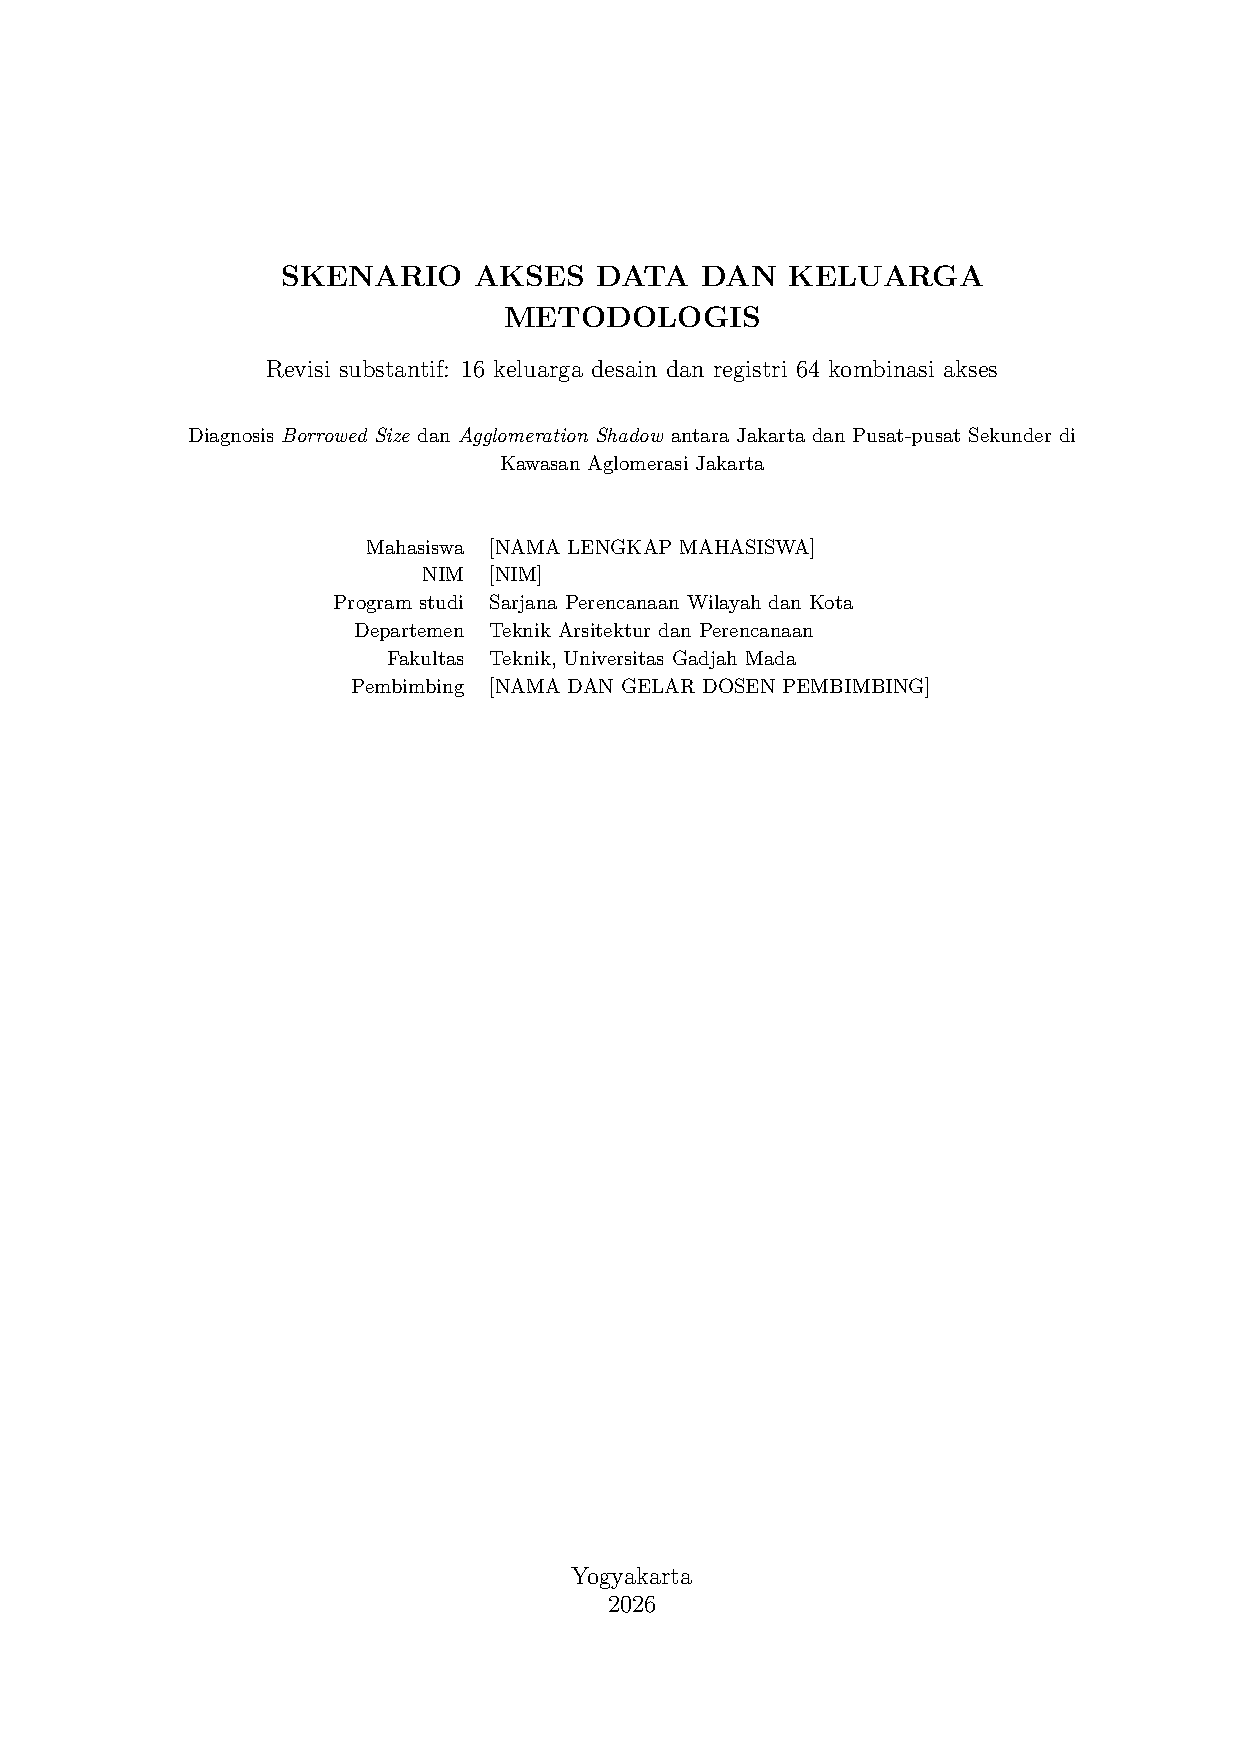
\includepdf[
  pages=-,
  pagecommand={\thispagestyle{empty}},
  addtotoc={1,chapter,1,{Bab 1: Skenario Akses Data dan Metodologi (Revisi)},bab:skenario}
]{../output/permohonan_data/skenario_akses_data_metodologis_revisi.pdf}
\clearpage

\chapter{\texorpdfstring{Bab 2 --- Dasar Teori dan Konsep Kunci
\emph{Borrowed Size} dan \emph{Agglomeration Shadow}
Jakarta}{Bab 2 --- Dasar Teori dan Konsep Kunci Borrowed Size dan Agglomeration Shadow Jakarta}}\label{bab-2-dasar-teori-dan-konsep-kunci-borrowed-size-dan-agglomeration-shadow-jakarta}

\begin{quote}
\textbf{Status dokumen:} catatan kerja untuk menyusun Bab 2, bukan
naskah final. Dokumen ini memetakan teori, konsep, penelitian terdahulu,
kerangka konseptual, dan daftar bacaan prioritas. Formulasi yang masih
perlu diuji melalui tinjauan pustaka sistematis ditandai sebagai
\textbf{kandidat}, bukan sebagai kesimpulan final.
\end{quote}

\section{Kedudukan dokumen}\label{kedudukan-dokumen}

Dokumen ini diturunkan dari arah penelitian dalam Skripsi S1 - Borrowed
Size dan Agglomeration Shadow Jakarta, struktur Bab 2 pada
\texttt{Template\ TGA\ Penelitian\ 2026.docx}, batas klaim dalam
output/permohonan_data/skenario_akses_data_metodologis_revisi.pdf dan
output/permohonan_data/skenario_akses_data_64.pdf, serta pilihan bacaan perencanaan
dalam output/atlas/atlas_masalah_mazhab_dan_sumber_keilmuan_urban_planning_interaktif.html.

Struktur template memisahkan tiga pekerjaan yang memang tampak mirip,
tetapi mempunyai fungsi berbeda:

{\def\LTcaptype{none} % do not increment counter
\begin{longtable}[]{@{}
  >{\raggedright\arraybackslash}p{(\linewidth - 6\tabcolsep) * \real{0.2500}}
  >{\raggedright\arraybackslash}p{(\linewidth - 6\tabcolsep) * \real{0.2500}}
  >{\raggedright\arraybackslash}p{(\linewidth - 6\tabcolsep) * \real{0.2500}}
  >{\raggedright\arraybackslash}p{(\linewidth - 6\tabcolsep) * \real{0.2500}}@{}}
\toprule\noalign{}
\begin{minipage}[b]{\linewidth}\raggedright
Bagian
\end{minipage} & \begin{minipage}[b]{\linewidth}\raggedright
Pertanyaan yang dijawab
\end{minipage} & \begin{minipage}[b]{\linewidth}\raggedright
Isi yang semestinya masuk
\end{minipage} & \begin{minipage}[b]{\linewidth}\raggedright
Hal yang perlu dihindari
\end{minipage} \\
\midrule\noalign{}
\endhead
\bottomrule\noalign{}
\endlastfoot
\textbf{2.1 Konsep-konsep kunci} & Apa arti istilah yang dipakai dalam
penelitian ini? & Definisi eksplisit dan pilihan definisi kerja &
Menumpuk banyak definisi tanpa memilih satu \\
\textbf{2.2 Penelitian terdahulu} & Apa yang sudah diketahui, bagaimana
cara mengetahuinya, dan apa yang belum dijawab? & Perbandingan fokus,
data, metode, temuan, keterbatasan, dan perbedaan penelitian & Menjadi
daftar ringkasan artikel yang tidak membentuk argumen kesenjangan \\
\textbf{2.3 Kerangka teori/konseptual} & Mengapa dan melalui mekanisme
apa antarkonsep dapat berhubungan? & Rantai mekanisme, konstruk,
indikator, proposisi, batas klaim, dan diagram & Mengulang definisi 2.1
atau langsung melompat ke indeks tanpa mekanisme \\
\end{longtable}
}

Dengan demikian, \textbf{konsep kunci adalah kosakata penelitian},
sedangkan \textbf{kerangka teori adalah tata hubungan dan mekanisme yang
menghubungkan kosakata tersebut}.

\section{Keputusan arsitektur
teoretis}\label{keputusan-arsitektur-teoretis}

Bab 2 sebaiknya tidak menjadikan \emph{borrowed size} sebagai
satu-satunya teori yang berdiri sendiri. Arsitektur yang paling dapat
dipertahankan secara akademik terdiri atas empat lapisan:

\begin{enumerate}
\def\labelenumi{\arabic{enumi}.}
\tightlist
\item
  \textbf{Ekonomi aglomerasi dan disekonomi aglomerasi} menjelaskan
  mengapa ukuran, kepadatan, dan kedekatan dapat menghasilkan manfaat
  sekaligus biaya.
\item
  \textbf{Polarisasi spasial dan kausasi kumulatif} menjelaskan mengapa
  pertumbuhan pusat besar dapat menyebar ke wilayah sekitar atau justru
  menarik sumber daya dari wilayah tersebut.
\item
  \textbf{Sistem perkotaan, polisentrisitas, spesialisasi fungsi, dan
  eksternalitas jaringan} menjelaskan bahwa manfaat metropolitan tidak
  hanya ditentukan oleh ukuran lokal, tetapi juga oleh posisi suatu
  pusat dalam jaringan antarkota.
\item
  \textbf{\emph{Borrowed size--agglomeration shadow}} menjadi kerangka
  diagnosis tingkat menengah yang menghubungkan integrasi jaringan
  dengan fungsi atau kinerja aktual relatif terhadap yang diharapkan
  dari ukuran lokal.
\end{enumerate}

Konsep aksesibilitas, geografi fungsional, pusat sekunder, kematangan
fungsi lokal, residu fungsi--ukuran, ketergantungan, dan skenario
sensitivitas berperan sebagai \textbf{konsep jembatan dan operasional}.
Teori \emph{post-suburbanization}, \emph{mega-urban region}, dan
\emph{desakota} dipakai sebagai \textbf{lensa kontekstual Jakarta},
bukan sebagai bukti otomatis terjadinya \emph{borrowed size} atau
\emph{agglomeration shadow}.

\subsection{Peta hubungan awal}\label{peta-hubungan-awal}

\begin{figure}[H]
\centering
\begin{adjustbox}{max width=\textwidth,max totalheight=0.84\textheight,center}
\begin{tikzpicture}[x=1cm,y=1cm]
  \node[diagbox] (A) at (-5,0) {Ukuran, kepadatan, dan karakteristik lokal};
  \node[diagbox] (C) at (0,0) {Arus aktual dan konektivitas antarpusat};
  \node[diagbox] (E) at (5,0) {Hierarki, spesialisasi, dan relasi inti--pinggiran};

  \node[diagbox] (B) at (-5,-2) {Ekspektasi fungsi berdasarkan ukuran lokal};
  \node[diagbox] (D) at (0,-2) {Akses ke sumber daya metropolitan};
  \node[diagbox] (F) at (5,-2) {Efek penyebaran, penarikan balik, atau pembagian fungsi};

  \node[diagbox] (H) at (-5,-4) {Residu fungsi: aktual dikurangi ekspektasi};
  \node[diagbox] (G) at (0,-4) {Fungsi atau kinerja aktual};
  \node[diagbox] (I) at (5,-4) {Derajat integrasi fungsional};

  \node[diagbox] (K) at (-5,-6) {Manfaat, beban, dan ketergantungan};
  \node[diagbox] (J) at (0,-6) {Diagnosis relasional};
  \node[diagbox] (O) at (5,-6) {Batas administrasi tetap};

  \node[diagbox,text width=52mm] (L) at (0,-8) {\emph{Borrowed size} / campuran / \emph{shadow} / independen / periferi lemah};
  \node[diagbox] (M) at (-5,-10) {Variasi indikator, bobot, dan ambang};
  \node[diagbox,text width=52mm] (N) at (0,-10) {Uji sensitivitas dan ketahanan};

  \draw[diagarrow] (A) -- (B);
  \draw[diagarrow] (C) -- (D);
  \draw[diagarrow] (E) -- (F);
  \draw[diagarrow] (D) -- (G);
  \draw[diagarrow] (F) -- (G);
  \draw[diagarrow] (B) -- (H);
  \draw[diagarrow] (G) -- (H);
  \draw[diagarrow] (C) to[bend left=12] (I);
  \draw[diagarrow] (H) -- (J);
  \draw[diagarrow] (I) -- (J);
  \draw[diagarrow] (K) -- (J);
  \draw[diagarrow] (J) -- (L);
  \draw[diagarrow] (O) -- (L);
  \draw[diagarrow] (L) -- (N);
  \draw[diagarrow] (M) -- (N);
  \draw[diagarrow] (O) to[bend left=14] (N);
\end{tikzpicture}
\end{adjustbox}
\caption{Peta hubungan awal untuk diagnosis \emph{borrowed size} dan \emph{agglomeration shadow}.}
\end{figure}

Diagram tersebut adalah \textbf{kerangka diagnosis}, bukan model
sebab-akibat yang sudah terbukti.

\section{2.1 Penjelasan konsep-konsep
kunci}\label{penjelasan-konsep-konsep-kunci}

\subsection{2.1.1 Ekonomi aglomerasi dan disekonomi
aglomerasi}\label{ekonomi-aglomerasi-dan-disekonomi-aglomerasi}

\textbf{Definisi kerja.} Ekonomi aglomerasi adalah manfaat yang
diperoleh rumah tangga atau perusahaan karena berlokasi dekat dengan
banyak orang, perusahaan, pekerja, pemasok, pengetahuan, infrastruktur,
dan amenitas. Duranton dan Puga merangkum mekanismenya sebagai
\textbf{berbagi (\emph{sharing}), mencocokkan (\emph{matching}), dan
belajar (\emph{learning})}: berbagi input atau fasilitas, mencocokkan
pasar kerja dan kebutuhan, serta memperoleh pembelajaran dan limpahan
pengetahuan. Disekonomi aglomerasi adalah biaya yang meningkat bersama
konsentrasi, seperti kemacetan, harga lahan dan perumahan, polusi,
tekanan infrastruktur, serta kompetisi yang menyingkirkan fungsi
tertentu.

\textbf{Peran dalam penelitian.} Teori ini memberi alasan mengapa ukuran
lokal perlu dijadikan garis dasar. Jika kota yang lebih besar secara
umum mampu menopang lebih banyak fungsi, maka \emph{borrowed size} tidak
dapat diidentifikasi hanya dari banyaknya fasilitas; fungsi aktual harus
dibandingkan dengan tingkat yang lazim untuk ukuran lokal yang setara.

\textbf{Batas penggunaan.} Aglomerasi tidak berarti semua dimensi
kinerja selalu meningkat bersama kepadatan. Hasil dapat berbeda menurut
sektor, fungsi, kelompok sosial, skala spasial, dan konteks negara.
Kepadatan juga bukan sinonim langsung dari produktivitas.

\subsection{2.1.2 Ukuran lokal, fungsi metropolitan, dan
kinerja}\label{ukuran-lokal-fungsi-metropolitan-dan-kinerja}

Tiga objek ini perlu dipisahkan:

\begin{itemize}
\tightlist
\item
  \textbf{ukuran lokal} adalah massa yang dimiliki unit itu sendiri,
  misalnya penduduk, tenaga kerja, jumlah usaha, atau kepadatan;
\item
  \textbf{fungsi metropolitan} adalah kapasitas unit menyediakan
  aktivitas atau layanan berorde lebih tinggi, misalnya pekerjaan
  tertentu, layanan khusus, fungsi bisnis, pendidikan, kesehatan,
  budaya, atau pusat kegiatan;
\item
  \textbf{kinerja} adalah hasil yang dicapai, misalnya produktivitas,
  pendapatan, inovasi, atau hasil kesejahteraan.
\end{itemize}

Sebuah pusat dapat berpenduduk besar tetapi mempunyai fungsi berorde
tinggi yang terbatas. Sebaliknya, pusat yang lebih kecil dapat mempunyai
fungsi lebih banyak daripada yang lazim bagi ukurannya. Karena itu,
penelitian ini tidak boleh memakai fasilitas, PDRB, atau jumlah
pekerjaan sebagai pengganti satu sama lain tanpa menjelaskan konstruk
yang sebenarnya diukur.

\subsection{2.1.3 Sistem perkotaan, hierarki pusat, dan pusat
sekunder}\label{sistem-perkotaan-hierarki-pusat-dan-pusat-sekunder}

\textbf{Sistem perkotaan} adalah himpunan pusat yang saling terkait
melalui arus manusia, barang, jasa, modal, informasi, dan pembagian
fungsi. Teori tempat sentral memberi titik awal untuk memahami hierarki:
layanan berorde lebih tinggi cenderung membutuhkan ambang permintaan dan
jangkauan pasar yang lebih besar. Literatur sistem kota dan jaringan
kemudian menunjukkan bahwa fungsi sebuah pusat tidak hanya bergantung
pada pasar lokal, tetapi juga pada posisi dan relasinya dengan pusat
lain.

\textbf{Definisi kerja pusat sekunder.} Pusat sekunder adalah pusat
selain inti Jakarta yang mempunyai konsentrasi penduduk, pekerjaan,
layanan, atau aktivitas dan berpotensi menjalankan fungsi subregional
atau metropolitan. Status ``sekunder'' harus ditentukan melalui kriteria
empiris yang konsisten, bukan sekadar karena unit tersebut bersebelahan
dengan Jakarta atau berstatus kota administratif.

\textbf{Catatan.} Teori tempat sentral berguna sebagai garis dasar
hierarki fungsi, tetapi asumsi pasar seragam dan ruang isotropiknya
terlalu sederhana untuk langsung diterapkan pada Jabodetabek.

\subsection{2.1.4 Polisentrisitas morfologis dan
fungsional}\label{polisentrisitas-morfologis-dan-fungsional}

\textbf{Polisentrisitas morfologis} menunjuk pada keberadaan beberapa
konsentrasi penduduk atau pekerjaan yang relatif berimbang.
\textbf{Polisentrisitas fungsional} menunjuk pada intensitas dan pola
hubungan antarpusat, misalnya arus komuter, perjalanan, transaksi, atau
jaringan organisasi.

Pembedaan ini krusial: adanya beberapa pusat pada peta tidak membuktikan
bahwa wilayah tersebut berfungsi sebagai jaringan yang terintegrasi.
Sebaliknya, hubungan kuat dengan Jakarta dapat tetap terjadi dalam
struktur yang hierarkis dan asimetris. Karena itu, penelitian tidak
boleh memakai ``banyak pusat'' sebagai sinonim dari pemerataan fungsi,
kemandirian, atau keberhasilan metropolitan.

\subsection{2.1.5 Aksesibilitas, konektivitas, dan integrasi
fungsional}\label{aksesibilitas-konektivitas-dan-integrasi-fungsional}

Ketiga istilah ini tidak identik:

\begin{itemize}
\tightlist
\item
  \textbf{aksesibilitas} adalah potensi menjangkau peluang dengan
  mempertimbangkan distribusi peluang dan hambatan perjalanan;
\item
  \textbf{konektivitas} adalah keberadaan dan kualitas hubungan dalam
  jaringan;
\item
  \textbf{integrasi fungsional} adalah hubungan yang benar-benar
  termanifestasi melalui arus atau interaksi aktual antarpusat.
\end{itemize}

Jika data hanya berisi waktu tempuh, jaringan jalan, atau jarak, hasil
harus disebut \textbf{aksesibilitas potensial}, bukan integrasi aktual.
Klaim integrasi lebih kuat memerlukan bukti relasional, seperti
asal--tujuan komuter, perjalanan, transaksi, jaringan perusahaan, atau
bentuk arus lain yang dapat dipertanggungjawabkan.

\subsection{2.1.6 Kematangan fungsi lokal dan residu
fungsi--ukuran}\label{kematangan-fungsi-lokal-dan-residu-fungsiukuran}

\textbf{Kematangan fungsi lokal} adalah kemampuan suatu pusat untuk
menopang kombinasi pekerjaan, layanan, dan aktivitas yang sepadan atau
lebih tinggi daripada basis ukuran dan karakteristik lokalnya. Ia tidak
sama dengan swasembada absolut dan tidak mengharuskan terputus dari
Jakarta.

Secara konseptual, untuk fungsi \(k\) pada unit \(i\):

\[
\widehat{F}_{ik}=f_k(S_i,X_i)
\]

\[
R_{ik}=F_{ik}-\widehat{F}_{ik}
\]

dengan:

\begin{itemize}
\tightlist
\item
  \(F_{ik}\): fungsi atau kinerja aktual yang benar-benar diukur;
\item
  \(S_i\): ukuran lokal;
\item
  \(X_i\): karakteristik pembanding yang relevan dan tersedia;
\item
  \(\widehat{F}_{ik}\): fungsi yang diharapkan berdasarkan unit
  pembanding atau model transparan;
\item
  \(R_{ik}\): residu berupa surplus atau defisit relatif pada konstruk
  \(k\).
\end{itemize}

Residu positif tidak otomatis membuktikan \emph{borrowed size}; residu
negatif tidak otomatis membuktikan \emph{shadow}. Keduanya baru bermakna
relasional ketika dibaca bersama integrasi dengan Jakarta atau jaringan
pusat lain.

\subsection{\texorpdfstring{2.1.7 \emph{Borrowed
size}}{2.1.7 Borrowed size}}\label{borrowed-size}

\textbf{Definisi teoretis.} \emph{Borrowed size} adalah keadaan ketika
suatu tempat memiliki fungsi atau tingkat kinerja yang lazimnya
diasosiasikan dengan kota yang lebih besar karena tempat tersebut dapat
mengakses dan memobilisasi manfaat aglomerasi melalui jaringan dengan
pusat lain. Alonso memperkenalkan intuisi awalnya, sedangkan Meijers dan
Burger memperluasnya dari kedekatan dalam kompleks metropolitan menjadi
hubungan jaringan pada berbagai skala.

\textbf{Definisi operasional sementara.} Suatu unit menunjukkan pola
yang konsisten dengan \emph{borrowed size} apabila:

\begin{enumerate}
\def\labelenumi{\arabic{enumi}.}
\tightlist
\item
  terdapat bukti hubungan aktual atau bukti relasional yang memadai
  dengan Jakarta atau jaringan pusat;
\item
  fungsi aktual menunjukkan surplus yang substantif terhadap ekspektasi
  berdasarkan ukuran dan karakteristik lokal;
\item
  unit, periode, wilayah tangkapan (\emph{catchment}), dan konstruk
  antara integrasi dan fungsi cukup kompatibel; dan
\item
  klasifikasi tidak runtuh hanya karena satu indikator, satu bobot, satu
  ambang, atau satu proksi bermutu rendah.
\end{enumerate}

Dengan desain potong lintang atau observasional nonkausal, formulasi
hasil yang aman adalah \textbf{``pola konsisten dengan borrowed size''},
bukan ``Jakarta menyebabkan pusat tersebut meminjam ukuran.''

\subsection{\texorpdfstring{2.1.8 \emph{Agglomeration
shadow}}{2.1.8 Agglomeration shadow}}\label{agglomeration-shadow}

\textbf{Definisi teoretis.} \emph{Agglomeration shadow} adalah keadaan
ketika posisi dekat atau terhubung dengan pusat yang dominan berkaitan
dengan fungsi atau kinerja lokal yang lebih rendah daripada yang
sewajarnya diharapkan, antara lain karena kompetisi permintaan, tenaga
terampil, investasi, atau fungsi berorde tinggi terkonsentrasi pada
pusat besar.

\textbf{Definisi operasional sementara.} Label ketat memerlukan empat
gerbang bukti yang sama dengan \emph{borrowed size}, tetapi residu
fungsinya negatif dan idealnya diperkuat oleh bukti beban atau
ketergantungan asimetris. Kedekatan, waktu tempuh singkat, arus keluar
komuter, atau defisit fasilitas secara sendiri-sendiri belum cukup.

\textbf{Bukti tandingan penting.} Literatur empiris menunjukkan bahwa
kedekatan ke pusat besar tidak selalu menekan pertumbuhan. Efek dapat
positif, negatif, tidak signifikan, atau berbeda menurut fungsi dan
posisi jaringan. Oleh sebab itu, \emph{shadow} harus diuji, bukan
diasumsikan.

\subsection{2.1.9 Spesialisasi fungsi dan ketergantungan
asimetris}\label{spesialisasi-fungsi-dan-ketergantungan-asimetris}

Duranton dan Puga menunjukkan bahwa organisasi ekonomi dapat berubah
dari spesialisasi menurut sektor menuju spesialisasi menurut fungsi:
kantor pusat dan layanan bisnis terkonsentrasi di kota besar, sedangkan
pabrik atau produksi berpindah ke kota yang lebih kecil. Implikasinya
bagi Jakarta adalah bahwa pertumbuhan pekerjaan industri di pinggiran
belum tentu identik dengan pematangan seluruh fungsi lokal.

\textbf{Ketergantungan asimetris} berarti hubungan dengan inti penting
bagi pusat sekunder, sementara kepentingan timbal baliknya tidak
seimbang. Ia dapat muncul melalui dominasi tujuan komuter,
ketergantungan pada layanan berorde tinggi di inti, konsentrasi fungsi
keputusan di Jakarta, atau beban infrastruktur dan lingkungan yang tidak
disertai penguatan kapasitas lokal.

Ketergantungan harus dilaporkan sebagai dimensi tersendiri. Manfaat
akses metropolitan dan ketergantungan dapat hadir secara bersamaan.

\subsection{\texorpdfstring{2.1.10 Kondisi campuran atau
\emph{contested}}{2.1.10 Kondisi campuran atau contested}}\label{kondisi-campuran-atau-contested}

Kategori campuran diperlukan untuk pusat yang:

\begin{itemize}
\tightlist
\item
  menikmati akses atau surplus pada satu fungsi tetapi mengalami defisit
  pada fungsi lain;
\item
  memiliki surplus fungsi sekaligus beban ketergantungan tinggi;
\item
  menunjukkan hasil yang berubah-ubah ketika indikator atau ambang
  diganti; atau
\item
  belum memenuhi gerbang bukti untuk label \emph{borrowed size} maupun
  \emph{shadow}.
\end{itemize}

Kategori ini bukan ``tempat sisa'', melainkan perlindungan terhadap
klasifikasi biner yang terlalu percaya diri.

\subsection{2.1.11 Geografi fungsional dan yurisdiksi
administratif}\label{geografi-fungsional-dan-yurisdiksi-administratif}

Geografi fungsional dibentuk oleh arus, jangkauan pasar, waktu tempuh,
dan wilayah tangkapan kegiatan. Yurisdiksi administratif menentukan
kewenangan, pelayanan, fiskal, dan akuntabilitas. Penelitian dapat
memetakan hubungan yang melintasi batas, tetapi tidak boleh menafsirkan
perluasan jejak fungsional sebagai perluasan wilayah administratif
Jakarta.

Pendekatan \emph{functional urban area} berguna sebagai referensi untuk
mengidentifikasi wilayah inti dan zona komuter, tetapi definisinya perlu
disesuaikan secara transparan dengan unit dan ketersediaan data
Indonesia.

\subsection{\texorpdfstring{2.1.12 Diagnosis \emph{status quo},
sensitivitas, dan
skenario}{2.1.12 Diagnosis status quo, sensitivitas, dan skenario}}\label{diagnosis-status-quo-sensitivitas-dan-skenario}

\begin{itemize}
\tightlist
\item
  \textbf{Diagnosis \emph{status quo}} menggunakan data observasi untuk
  menggambarkan integrasi, fungsi relatif, manfaat, beban, dan kelas
  dasar.
\item
  \textbf{Analisis sensitivitas} mengubah asumsi teknis---indikator,
  bobot, ambang, atau spesifikasi model---untuk menguji kestabilan
  hasil.
\item
  \textbf{Skenario} adalah konfigurasi nilai atau asumsi yang eksplisit
  untuk mengeksplorasi konsekuensi kondisional; ia bukan ramalan dan
  bukan bukti perubahan kausal.
\end{itemize}

Literatur \emph{planning support systems} membantu merancang antarmuka
yang membuat asumsi, hasil dasar, perubahan kelas, dan ketidakpastian
terlihat. WebGL adalah medium komunikasi dan eksplorasi model, bukan
teori substantif tentang metropolitan Jakarta.

\section{2.2 Kajian penelitian
terdahulu}\label{kajian-penelitian-terdahulu}

\subsection{2.2.1 Sintesis menurut rumpun
literatur}\label{sintesis-menurut-rumpun-literatur}

{\def\LTcaptype{none} % do not increment counter
\begin{longtable}[]{@{}
  >{\raggedright\arraybackslash}p{(\linewidth - 6\tabcolsep) * \real{0.2500}}
  >{\raggedright\arraybackslash}p{(\linewidth - 6\tabcolsep) * \real{0.2500}}
  >{\raggedright\arraybackslash}p{(\linewidth - 6\tabcolsep) * \real{0.2500}}
  >{\raggedright\arraybackslash}p{(\linewidth - 6\tabcolsep) * \real{0.2500}}@{}}
\toprule\noalign{}
\begin{minipage}[b]{\linewidth}\raggedright
Rumpun
\end{minipage} & \begin{minipage}[b]{\linewidth}\raggedright
Yang telah ditunjukkan literatur
\end{minipage} & \begin{minipage}[b]{\linewidth}\raggedright
Batas yang relevan
\end{minipage} & \begin{minipage}[b]{\linewidth}\raggedright
Implikasi untuk penelitian
\end{minipage} \\
\midrule\noalign{}
\endhead
\bottomrule\noalign{}
\endlastfoot
Asal dan perluasan \emph{borrowed size} & Pusat kecil dapat memiliki
fungsi/kinerja di atas ekspektasi ukuran melalui jaringan; skala dan
fungsi penting & Basis empiris awal didominasi Eropa dan hasilnya
bergantung pada jenis fungsi & Uji per fungsi dan jangan menganggap
transfer ke Jakarta otomatis \\
Operasionalisasi fungsi--ukuran & Fungsi aktual dapat dibandingkan
dengan hubungan umum antara ukuran kota dan fungsi & Residu dapat
berubah menurut unit, model, dan proksi & Gunakan model pembanding yang
transparan serta diagnostik sensitivitas \\
\emph{Agglomeration shadow} & Pusat dominan dapat menaungi pusat lain,
tetapi kedekatan juga dapat menghasilkan limpahan positif & Bukti tidak
universal dan tidak semua studi mengukur hubungan aktual & Perlakukan
\emph{shadow} sebagai hipotesis relasional, bukan efek jarak \\
Polisentrisitas dan jaringan kota & Morfologi dan fungsi merupakan
dimensi berbeda; integrasi dapat memperkuat akses pada fungsi
metropolitan & Banyak pusat tidak otomatis berarti jaringan kohesif atau
kinerja tinggi & Arus aktual harus dipisahkan dari jumlah dan ukuran
pusat \\
Aglomerasi dan spesialisasi fungsi & Manfaat aglomerasi bekerja melalui
mekanisme berbagi--mencocokkan--belajar; fungsi keputusan dan produksi
dapat terpisah & Produktivitas, fasilitas, pekerjaan, dan kesejahteraan
bukan konstruk yang identik & Pilih indikator sesuai konstruk dan
laporkan hasil secara multidimensi \\
Transformasi metropolitan Jakarta & Terjadi suburbanisasi industri, kota
baru, transformasi peri-urban, privatisasi, dan kecenderungan
multisentris & Sebagian studi bersifat deskriptif atau menekankan
morfologi, tata guna lahan, dan satu sektor & Menyediakan konteks,
tetapi belum langsung mengklasifikasikan \emph{borrowed size--shadow} \\
Mobilitas dan post-suburbanisasi Jakarta & Arus komuter memperlihatkan
hubungan inti--pinggiran dan antarpinggiran yang berubah & Skala data
dan periode tertentu membatasi generalisasi & Menunjukkan pentingnya
bukti arus untuk integrasi dan kematangan pusat \\
\end{longtable}
}

\subsection{2.2.2 Kandidat kesenjangan
penelitian}\label{kandidat-kesenjangan-penelitian}

Berdasarkan penelusuran awal, literatur Jakarta telah membahas
dekonsentrasi industri, perkembangan kota baru, transformasi periurban,
polisentrisitas morfologis/fungsional, dan komuter. Literatur
\emph{borrowed size} telah mengembangkan hubungan antara ukuran,
konektivitas jaringan, fungsi, dan \emph{shadow}, terutama di Eropa.

\textbf{Kandidat kesenjangan} penelitian ini adalah belum ditemukannya
studi Jakarta yang secara bersamaan:

\begin{enumerate}
\def\labelenumi{\arabic{enumi}.}
\tightlist
\item
  mengukur integrasi relasional pusat sekunder dengan Jakarta dan pusat
  lain;
\item
  membandingkan fungsi aktual dengan ekspektasi berdasarkan ukuran dan
  karakteristik lokal;
\item
  memisahkan surplus/defisit fungsi, manfaat akses, dan beban
  ketergantungan;
\item
  membentuk tipologi \emph{borrowed size--campuran--shadow} beserta
  kelas pembanding; dan
\item
  menguji kestabilan jejak spasial klasifikasi terhadap pilihan
  indikator, bobot, ambang, serta spesifikasi model dengan batas
  administratif tetap.
\end{enumerate}

Rumusan ini \textbf{belum boleh ditulis sebagai kesenjangan final}
sebelum pencarian bibliografi yang lebih sistematis---termasuk literatur
Indonesia yang mungkin tidak terindeks baik---selesai dilakukan.

\subsection{2.2.3 Matriks penelitian Jakarta yang paling
relevan}\label{matriks-penelitian-jakarta-yang-paling-relevan}

{\def\LTcaptype{none} % do not increment counter
\begin{longtable}[]{@{}
  >{\raggedright\arraybackslash}p{(\linewidth - 6\tabcolsep) * \real{0.2500}}
  >{\raggedright\arraybackslash}p{(\linewidth - 6\tabcolsep) * \real{0.2500}}
  >{\raggedright\arraybackslash}p{(\linewidth - 6\tabcolsep) * \real{0.2500}}
  >{\raggedright\arraybackslash}p{(\linewidth - 6\tabcolsep) * \real{0.2500}}@{}}
\toprule\noalign{}
\begin{minipage}[b]{\linewidth}\raggedright
Sumber
\end{minipage} & \begin{minipage}[b]{\linewidth}\raggedright
Fokus/data utama
\end{minipage} & \begin{minipage}[b]{\linewidth}\raggedright
Kontribusi untuk skripsi
\end{minipage} & \begin{minipage}[b]{\linewidth}\raggedright
Perbedaan yang perlu dipertahankan
\end{minipage} \\
\midrule\noalign{}
\endhead
\bottomrule\noalign{}
\endlastfoot
Henderson, Kuncoro, \& Nasution (1996) & Pergeseran residensi dan
industri Jabotabek; perubahan dari monosentris ke multisentris & Dasar
historis restrukturisasi pusat dan pekerjaan & Belum memakai kerangka
\emph{borrowed size--shadow} atau residu fungsi--ukuran \\
Firman (2009) & Mega-urbanisasi koridor Jakarta--Bandung dan perubahan
multi-inti & Menempatkan Jakarta dalam sistem urban yang meluas &
Transformasi bentuk tidak otomatis menunjukkan integrasi produktif \\
Hudalah \& Firman (2012) & Kawasan industri dan elemen
\emph{post-suburbia} & Menunjukkan dekonsentrasi fungsi ekonomi ke
pinggiran & Fokus sektoral dan transformasi kawasan, bukan diagnosis
fungsi relatif \\
Hudalah et al.~(2013) & Dekonsetrasi manufaktur dan pusat industri
privat & Bukti bahwa pusat industri pinggiran menangkap pekerjaan
manufaktur & Pekerjaan manufaktur tidak boleh disamakan dengan seluruh
kematangan fungsi \\
Winarso, Hudalah, \& Firman (2015) & Transformasi sosial-ekonomi
peri-urban dan segregasi & Menghubungkan pertumbuhan dengan distribusi
manfaat dan ketimpangan & Perlu memisahkan manfaat, fungsi, dan beban
pada unit analisis penelitian ini \\
Firman \& Fahmi (2017) & Privatisasi pinggiran, kota baru, dan fase awal
\emph{post-suburbanization} & Konteks perkembangan pusat pinggiran yang
lebih mandiri & Pendekatan deskriptif; tidak membuktikan \emph{borrowed
size} \\
Sadewo et al.~(2021) & Polisentrisitas morfologis dan fungsional Medan,
Jakarta, Denpasar & Dasar operasional pemisahan pusat dan hubungan
antarpusat & Polisentrisitas bukan sinonim surplus fungsi atau rendahnya
ketergantungan \\
Sadewo et al.~(2023) & Panel spasial komuter antarpinggiran 2008--2015 &
Bukti interaksi antarpinggiran dan pengaruh dekonsentrasi pekerjaan &
Fokus komuter; perlu ditautkan ke fungsi relatif dan beban \\
Aritenang (2023) & Survei komuter 2014 dan 2019; independensi,
kematangan, segregasi & Sumber terdekat untuk konstruksi kematangan
pusat dan relasi komuter & Kerangka \emph{post-suburbanization}, bukan
klasifikasi \emph{borrowed size--shadow} \\
\end{longtable}
}

\section{2.3 Kerangka teori dan kerangka
konseptual}\label{kerangka-teori-dan-kerangka-konseptual}

\subsection{2.3.1 Rantai mekanisme}\label{rantai-mekanisme}

\subsubsection{Mekanisme A --- Manfaat dan biaya ukuran
lokal}\label{mekanisme-a-manfaat-dan-biaya-ukuran-lokal}

Ukuran dan kepadatan lokal dapat meningkatkan variasi pemasok, pasar
tenaga kerja, peluang pencocokan, pembelajaran, infrastruktur bersama,
dan permintaan terhadap fungsi berorde tinggi. Pada saat yang sama,
konsentrasi meningkatkan biaya lahan, kemacetan, polusi, dan kompetisi.
Hubungan antara ukuran dan fungsi menjadi garis dasar yang perlu
diestimasi, bukan diasumsikan linear dan seragam.

\subsubsection{Mekanisme B --- Eksternalitas jaringan dan peminjaman
ukuran}\label{mekanisme-b-eksternalitas-jaringan-dan-peminjaman-ukuran}

Pusat yang terhubung dapat mengakses pasar, tenaga kerja, pengetahuan,
fasilitas, dan fungsi di luar ukuran lokalnya. Jaringan dapat menjadi
pelengkap atau sebagian substitusi bagi kedekatan internal. Efeknya
bergantung pada kualitas konektivitas, arus aktual, fungsi yang diukur,
ukuran pusat itu sendiri, dan kemampuan lokal menyerap manfaat.

\subsubsection{\texorpdfstring{Mekanisme C --- Polarisasi,
\emph{backwash}, dan pembagian
fungsi}{Mekanisme C --- Polarisasi, backwash, dan pembagian fungsi}}\label{mekanisme-c-polarisasi-backwash-dan-pembagian-fungsi}

Keterhubungan juga dapat memusatkan permintaan, fungsi keputusan, tenaga
terampil, modal, dan layanan berorde tinggi pada Jakarta. Pusat
pinggiran dapat tumbuh sebagai lokasi produksi atau perumahan tanpa
memperoleh fungsi pengendalian, layanan strategis, atau kapasitas fiskal
yang sebanding. Karena itu, pertumbuhan absolut dapat hadir bersamaan
dengan defisit fungsi relatif atau beban tinggi.

\subsubsection{Mekanisme D --- Struktur urban dan kondisi
perantara}\label{mekanisme-d-struktur-urban-dan-kondisi-perantara}

Efek jaringan dimoderasi oleh ukuran pusat sendiri, hierarki,
spesialisasi, posisi dalam jaringan, akses multimoda, struktur ekonomi,
ketersediaan lahan, institusi, dan batas administratif. Satu pusat dapat
meminjam fungsi tertentu, tetap bergantung pada fungsi lain, dan
terbebani pada dimensi ketiga.

\subsection{2.3.2 Model pengukuran
konseptual}\label{model-pengukuran-konseptual}

Untuk setiap pusat \(i\) dan dimensi fungsi \(k\), penelitian
membedakan:

\begin{enumerate}
\def\labelenumi{\arabic{enumi}.}
\tightlist
\item
  \textbf{Ukuran dan karakteristik lokal}: \(S_i, X_i\);
\item
  \textbf{Integrasi relasional}: \(I_i\), idealnya berasal dari arus
  aktual;
\item
  \textbf{Fungsi atau kinerja aktual}: \(F_{ik}\);
\item
  \textbf{Fungsi yang diharapkan}: \(\widehat{F}_{ik}\);
\item
  \textbf{Residu fungsi relatif}: \(R_{ik}\);
\item
  \textbf{Manfaat akses}: \(A_{ik}\);
\item
  \textbf{Beban atau ketergantungan}: \(D_{ik}\);
\item
  \textbf{Ketahanan klasifikasi}: \(Q_i\), diperoleh dari variasi
  spesifikasi yang masuk akal.
\end{enumerate}

Hubungan inti yang diuji adalah:

\[
R_{ik}=g_k(I_i,S_i,X_i,Z_i)+\varepsilon_{ik}
\]

dengan \(Z_i\) sebagai moderator kontekstual. Persamaan ini adalah
bentuk umum. Spesifikasi akhirnya harus mengikuti data dan desain Bab 3;
persamaan tidak mengharuskan regresi kausal apabila data hanya mendukung
diagnosis deskriptif.

\subsection{2.3.3 Tipologi diagnosis
sementara}\label{tipologi-diagnosis-sementara}

{\def\LTcaptype{none} % do not increment counter
\begin{longtable}[]{@{}
  >{\raggedright\arraybackslash}p{(\linewidth - 8\tabcolsep) * \real{0.1765}}
  >{\raggedleft\arraybackslash}p{(\linewidth - 8\tabcolsep) * \real{0.2353}}
  >{\raggedleft\arraybackslash}p{(\linewidth - 8\tabcolsep) * \real{0.2353}}
  >{\raggedright\arraybackslash}p{(\linewidth - 8\tabcolsep) * \real{0.1765}}
  >{\raggedright\arraybackslash}p{(\linewidth - 8\tabcolsep) * \real{0.1765}}@{}}
\toprule\noalign{}
\begin{minipage}[b]{\linewidth}\raggedright
Integrasi relasional
\end{minipage} & \begin{minipage}[b]{\linewidth}\raggedleft
Residu fungsi
\end{minipage} & \begin{minipage}[b]{\linewidth}\raggedleft
Beban atau ketergantungan
\end{minipage} & \begin{minipage}[b]{\linewidth}\raggedright
Kelas sementara
\end{minipage} & \begin{minipage}[b]{\linewidth}\raggedright
Interpretasi aman
\end{minipage} \\
\midrule\noalign{}
\endhead
\bottomrule\noalign{}
\endlastfoot
Tinggi & Positif & Rendah--sedang & \emph{Borrowed size} / integrasi
produktif & Pola konsisten dengan akses jaringan yang memperbesar fungsi
relatif \\
Tinggi & Positif & Tinggi & Campuran/\allowbreak{}\emph{contested} &
Surplus fungsi hadir, tetapi manfaat disertai ketergantungan atau beban
besar \\
Tinggi & Negatif & Tinggi & \emph{Agglomeration shadow} / ketergantungan
asimetris & Pola konsisten dengan integrasi yang tidak diikuti
pematangan fungsi lokal \\
Tinggi & Negatif & Rendah atau belum terbukti & Terintegrasi tetapi
tertinggal/belum pasti & Belum cukup bukti untuk menyebut
\emph{shadow} \\
Rendah & Positif & Bervariasi & Relatif independen atau matang lokal &
Surplus fungsi tidak terutama dibaca sebagai hasil hubungan dengan
Jakarta \\
Rendah & Negatif & Bervariasi & Periferi lemah & Basis lokal dan
hubungan metropolitan sama-sama terbatas \\
\end{longtable}
}

Kelas akhir sebaiknya dibuat per dimensi terlebih dahulu. Indeks
komposit hanya layak dibuat setelah arah indikator, skala, kualitas
data, korelasi antarkonstruk, dan sensitivitas bobot diperiksa.

\subsection{2.3.4 Proposisi empiris
kandidat}\label{proposisi-empiris-kandidat}

Jika desain Bab 3 mendukung pengujian inferensial, proposisi berikut
dapat diubah menjadi hipotesis. Jika tidak, gunakan sebagai ekspektasi
interpretif.

\begin{enumerate}
\def\labelenumi{\arabic{enumi}.}
\tightlist
\item
  \textbf{P1 --- Efek jaringan bersyarat.} Setelah ukuran dan
  karakteristik lokal diperhitungkan, integrasi fungsional yang lebih
  kuat berasosiasi dengan surplus pada sebagian fungsi, tetapi tidak
  harus pada semua fungsi.
\item
  \textbf{P2 --- Kemungkinan \emph{shadow}.} Pada pusat tertentu,
  integrasi kuat dengan Jakarta berasosiasi dengan defisit fungsi
  relatif dan/atau beban ketergantungan yang lebih tinggi.
\item
  \textbf{P3 --- Heterogenitas fungsi.} Arah dan besar hubungan berbeda
  antara pekerjaan, layanan, amenitas, fungsi keputusan, dan konstruk
  kinerja.
\item
  \textbf{P4 --- Peran \emph{own mass} dan posisi jaringan.} Pusat
  dengan basis lokal, sentralitas, dan kapasitas penyerapan yang lebih
  kuat lebih mampu mengubah akses jaringan menjadi pematangan fungsi
  lokal.
\item
  \textbf{P5 --- Morfologi tidak cukup.} Tingkat polisentrisitas
  morfologis tidak dengan sendirinya menjelaskan integrasi fungsional,
  surplus fungsi, atau rendahnya ketergantungan.
\item
  \textbf{P6 --- Ketidakpastian klasifikasi.} Sebagian unit akan
  berpindah kelas ketika proksi, bobot, ambang, atau wilayah tangkapan
  diubah; unit yang stabil lebih layak menjadi dasar kesimpulan
  kebijakan.
\end{enumerate}

\subsection{2.3.5 Gerbang penggunaan label
ketat}\label{gerbang-penggunaan-label-ketat}

Label \emph{borrowed size} atau \emph{agglomeration shadow} hanya
digunakan jika empat syarat terpenuhi:

\begin{enumerate}
\def\labelenumi{\arabic{enumi}.}
\tightlist
\item
  \textbf{Bukti relasional:} ada hubungan dengan Jakarta, bukan hanya
  kedekatan atau waktu tempuh.
\item
  \textbf{Pembanding substantif:} fungsi aktual dibandingkan dengan
  ekspektasi ukuran pada unit yang memadai.
\item
  \textbf{Kompatibilitas:} unit, periode, wilayah tangkapan, populasi
  sasaran, dan konstruk cukup sepadan.
\item
  \textbf{Ketahanan:} hasil tidak bergantung pada satu proksi lemah atau
  satu keputusan teknis.
\end{enumerate}

Jika salah satu syarat utama tidak terpenuhi, gunakan istilah seperti
``aksesibilitas potensial'', ``surplus/defisit fungsi relatif'',
``ketergantungan komuter'', atau ``pola belum terklasifikasi'', sesuai
bukti yang benar-benar tersedia.

\subsection{2.3.6 Klaim yang dapat dan tidak dapat
dibuat}\label{klaim-yang-dapat-dan-tidak-dapat-dibuat}

\textbf{Dapat dibuat dengan desain \emph{status quo} dan sensitivitas:}
pola spasial, asosiasi, arus, aksesibilitas potensial, surplus/defisit
relatif, tipologi relasional, multidimensionalitas, serta kestabilan
klasifikasi.

\textbf{Belum dapat dibuat tanpa desain tambahan:} Jakarta secara kausal
``mengisap'' pusat tertentu; integrasi menyebabkan produktivitas;
perubahan bobot pada WebGL memprediksi masa depan; terdapat radius
optimal universal; atau batas administratif harus diubah.

\section{Daftar bacaan prioritas}\label{daftar-bacaan-prioritas}

Daftar berikut disusun untuk dibaca, bukan sebagai pernyataan bahwa
seluruh teks lengkapnya sudah diakses. Urutan menunjukkan kegunaan bagi
skripsi, bukan peringkat mutu universal. Tidak dilakukan penyaringan
berdasarkan status gratis atau berbayar, sesuai kebutuhan awal.

\subsection{A. Lima belas bacaan
pertama}\label{a.-lima-belas-bacaan-pertama}

\begin{enumerate}
\def\labelenumi{\arabic{enumi}.}
\tightlist
\item
  \textbf{Meijers, E., \& Burger, M. (2017).
  \href{https://doi.org/10.1177/0042098015597642}{``Stretching the
  concept of `borrowed size'\,''}.} Bacaan konseptual utama untuk
  definisi \emph{borrowed size}, perluasan skala, fungsi, kinerja, dan
  peran jaringan.
\item
  \textbf{Meijers, E., Burger, M., \& Hoogerbrugge, M. (2016).
  \href{https://doi.org/10.1111/pirs.12181}{``Borrowing size in networks
  of cities: City size, network connectivity and metropolitan functions
  in Europe''}.} Dasar hubungan ukuran lokal, konektivitas, dan fungsi
  metropolitan.
\item
  \textbf{Burger, M., Meijers, E., Hoogerbrugge, M., \& Masip Tresserra,
  J. (2015).
  \href{https://doi.org/10.1080/09654313.2014.905002}{``Borrowed Size,
  Agglomeration Shadows and Cultural Amenities in North-West Europe''}.}
  Contoh langsung operasionalisasi fungsi--ukuran dan \emph{shadow};
  perlu dibaca dengan kesadaran bahwa amenitas budaya hanya satu
  konstruk.
\item
  \textbf{Alonso, W. (1973).
  \href{https://www.jstor.org/stable/20024174}{``Urban Zero Population
  Growth''}.} Sumber intuisi awal \emph{borrowed size} dalam kompleks
  metropolitan.
\item
  \textbf{Burger, M., \& Meijers, E. (2016).
  \href{https://doi.org/10.1111/pirs.12223}{``Agglomerations and the
  rise of urban network externalities''}.} Jembatan antara ekonomi
  aglomerasi dan manfaat posisi dalam jaringan kota.
\item
  \textbf{Duranton, G., \& Puga, D. (2004).
  \href{https://doi.org/10.1016/S1574-0080(04)80005-1}{``Micro-foundations
  of urban agglomeration economies''}.} Landasan mekanisme
  berbagi--mencocokkan--belajar.
\item
  \textbf{Duranton, G., \& Puga, D. (2020).
  \href{https://doi.org/10.1257/jep.34.3.3}{``The Economics of Urban
  Density''}.} Ringkasan modern manfaat dan biaya kepadatan; berguna
  untuk menahan narasi aglomerasi yang hanya positif.
\item
  \textbf{Myrdal, G. (1957).
  \href{https://books.google.com/books?id=aujSAAAAMAAJ}{\emph{Economic
  Theory and Under-developed Regions}}.} Landasan \emph{spread effects},
  \emph{backwash effects}, dan kausasi kumulatif. Catatan vault:
  source/book/Myrdal - 1957 - Economic Theory and Under-Developed
  Regions.
\item
  \textbf{Partridge, M. D., Rickman, D. S., Ali, K., \& Olfert, M. R.
  (2009). \href{https://doi.org/10.1111/j.1435-5957.2008.00211.x}{``Do
  New Economic Geography agglomeration shadows underlie current
  population dynamics across the urban hierarchy?''}.} Counterevidence
  penting: kedekatan ke pusat besar tidak otomatis menghasilkan
  \emph{shadow}.
\item
  \textbf{Burger, M., \& Meijers, E. (2012).
  \href{https://doi.org/10.1177/0042098011407095}{``Form Follows
  Function? Linking Morphological and Functional Polycentricity''}.}
  Dasar pemisahan polisentrisitas morfologis dan fungsional.
\item
  \textbf{Duranton, G., \& Puga, D. (2005).
  \href{https://doi.org/10.1016/j.jue.2004.12.002}{``From sectoral to
  functional urban specialisation''}.} Mekanisme penting untuk
  membedakan pertumbuhan produksi pinggiran dari pematangan fungsi
  keputusan dan layanan.
\item
  \textbf{Geurs, K. T., \& van Wee, B. (2004).
  \href{https://doi.org/10.1016/j.jtrangeo.2003.10.005}{``Accessibility
  evaluation of land-use and transport strategies: Review and research
  directions''}.} Dasar memilih dan membatasi makna indikator
  aksesibilitas.
\item
  \textbf{Firman, T., \& Fahmi, F. Z. (2017).
  \href{https://doi.org/10.1080/01944363.2016.1249010}{``The
  Privatization of Metropolitan Jakarta's (Jabodetabek) Urban
  Fringes''}.} Konteks utama perkembangan pusat pinggiran, kota baru,
  kawasan industri, dan \emph{post-suburbanization}. Catatan vault:
  source/journal/Firman - 2017 - Privatization of Metropolitan Jakarta
  Urban Fringes.
\item
  \textbf{Sadewo, E., Hudalah, D., Antipova, A., Cheng, L., \& Syabri,
  I. (2023). \href{https://doi.org/10.1080/02723638.2022.2125649}{``The
  role of urban transformation on inter-suburban commuting''}.} Bukti
  empiris tentang dekonsentrasi pekerjaan dan arus komuter
  antarpinggiran Jakarta.
\item
  \textbf{Aritenang, A. F. (2023).
  \href{https://doi.org/10.1016/j.habitatint.2023.102857}{``Identifying
  post-suburbanization: The case of the Jakarta metropolitan area''}.}
  Bacaan terdekat untuk independensi spasial, kematangan wilayah
  pinggiran, segregasi, dan data komuter 2014--2019.
\end{enumerate}

\subsubsection{Rute baca minimum bila waktu
terbatas}\label{rute-baca-minimum-bila-waktu-terbatas}

Baca berurutan: \textbf{Meijers \& Burger (2017) → Meijers et al.~(2016)
→ Burger et al.~(2015) → Duranton \& Puga (2004) → Myrdal (1957) →
Burger \& Meijers (2012) → Firman \& Fahmi (2017) → Sadewo et al.~(2023)
→ Aritenang (2023)}.

\subsection{B. Bacaan penguat dan penguji
argumen}\label{b.-bacaan-penguat-dan-penguji-argumen}

\begin{itemize}
\tightlist
\item
  \textbf{Krugman, P. (1991).
  \href{https://doi.org/10.1086/261763}{``Increasing Returns and
  Economic Geography''}.} Landasan \emph{new economic geography} untuk
  interaksi \emph{increasing returns}, biaya transportasi, dan pemusatan
  kegiatan.
\item
  \textbf{Fujita, M., Krugman, P., \& Venables, A. J. (1999).
  \href{https://mitpress.mit.edu/9780262561471/the-spatial-economy/}{\emph{The
  Spatial Economy: Cities, Regions, and International Trade}}.} Sintesis
  teoretis aglomerasi pada berbagai skala; berguna sebagai dasar
  mekanisme, bukan sebagai model empiris yang langsung dipindahkan ke
  Jakarta.
\item
  \textbf{Phelps, N. A., Fallon, R. J., \& Williams, C. L. (2001).
  \href{https://doi.org/10.1080/00343400120075885}{``Small Firms,
  Borrowed Size and the Urban--Rural Shift''}.} Aplikasi awal
  \emph{borrowed size} pada perusahaan kecil dan perubahan urban--rural.
\item
  \textbf{Arthur, W. B. (1990).
  \href{https://doi.org/10.1016/0165-4896(90)90064-E}{``\,`Silicon
  Valley' locational clusters: When do increasing returns imply
  monopoly?''}.} Latar mekanisme increasing returns dan konsentrasi yang
  sering dirujuk dalam genealogi \emph{shadow}.
\item
  \textbf{Dobkins, L. H., \& Ioannides, Y. M. (2001).
  \href{https://doi.org/10.1016/S0166-0462(01)00067-9}{``Spatial
  interactions among U.S. cities: 1900--1990''}.} Pengujian kedekatan
  dengan kota berhierarki lebih tinggi; hasil tidak selalu signifikan.
\item
  \textbf{Sohn, C., Licheron, J., \& Meijers, E. (2022).
  \href{https://doi.org/10.1111/pirs.12653}{``Border cities: Out of the
  shadow''}.} Menunjukkan bahwa batas dan integrasi pasar dapat
  memoderasi hubungan \emph{borrowing--shadowing}.
\item
  \textbf{Volgmann, K., \& Rusche, K. (2020).
  \href{https://doi.org/10.1111/tesg.12362}{``The Geography of Borrowing
  Size: Exploring Spatial Distributions for German Urban Regions''}.}
  Mengoperasionalkan \emph{borrowed size}, \emph{borrowed performance},
  \emph{borrowed function}, dan \emph{agglomeration shadow} pada unit
  lokal; sangat berguna untuk merancang tipologi.
\item
  \textbf{Kwon, Y.-H. (2026).
  \href{https://doi.org/10.1111/tesg.70061}{``Borrowed Size of Small and
  Medium Cities in a Hierarchical Urban System''}.} Perluasan terbaru ke
  sistem perkotaan Korea yang hierarkis; relevan sebagai penguji
  transfer dari konteks Eropa, bukan sebagai dasar klasik.
\item
  \textbf{Meijers, E., Hoogerbrugge, M., \& Cardoso, R. (2018).
  \href{https://doi.org/10.1111/tesg.12292}{``Beyond Polycentricity:
  Does Stronger Integration Between Cities in Polycentric Urban Regions
  Improve Performance?''}.} Integrasi fungsional, institusional, dan
  kultural; relevan untuk membedakan bentuk dari kohesi jaringan.
\item
  \textbf{Meijers, E. (2008).
  \href{https://doi.org/10.1080/09654310802401805}{``Measuring
  Polycentricity and its Promises''}.} Kritik terhadap ambiguitas dan
  basis empiris polisentrisitas. Catatan vault: source/journal/Meijers -
  2008 - Measuring Polycentricity and its Promises.
\item
  \textbf{Meijers, E. J., \& Burger, M. J. (2010).
  \href{https://doi.org/10.1068/a42151}{``Spatial Structure and
  Productivity in US Metropolitan Areas''}.} Bukti komparatif bahwa
  struktur spasial dapat berkaitan dengan produktivitas, tetapi temuan
  AS tidak boleh ditransfer langsung. Catatan vault:
  source/journal/Meijers - 2010 - Spatial Structure and Productivity in
  US Metropolitan Areas.
\item
  \textbf{Rosenthal, S. S., \& Strange, W. C. (2004).
  \href{https://doi.org/10.1016/S1574-0080(04)80006-3}{``Evidence on the
  Nature and Sources of Agglomeration Economies''}.} Tinjauan bukti
  empiris aglomerasi.
\item
  \textbf{Ahlfeldt, G. M., \& Pietrostefani, E. (2019).
  \href{https://doi.org/10.1016/j.jue.2019.04.006}{``The economic
  effects of density: A synthesis''}.} Sintesis kuantitatif efek
  kepadatan.
\item
  \textbf{Grover, A., Lall, S. V., \& Timmis, J. (2023).
  \href{https://doi.org/10.1016/j.regsciurbeco.2023.103901}{``Agglomeration
  economies in developing countries: A meta-analysis''}.} Penguji
  transfer teori aglomerasi ke konteks negara berkembang.
\item
  \textbf{Christaller, W. (1966 {[}1933{]}).
  \href{https://books.google.com/books/about/Central_places_in_southern_Germany.html?id=BONEAAAAIAAJ}{\emph{Central
  Places in Southern Germany}}.} Dasar hierarki pusat, ambang, dan
  jangkauan fungsi. Catatan vault: source/book/Christaller - 1933 - Die
  zentralen Orte in Süddeutschland.
\item
  \textbf{Mulligan, G. F., Partridge, M. D., \& Carruthers, J. I.
  (2012). \href{https://doi.org/10.1007/s00168-011-0496-7}{``Central
  place theory and its reemergence in regional science''}.} Jembatan
  dari teori tempat sentral klasik ke ilmu regional kontemporer.
\item
  \textbf{Hirschman, A. O. (1958).
  \href{https://books.google.com/books/about/The_Strategy_of_Economic_Development.html?id=wls-AAAAYAAJ}{\emph{The
  Strategy of Economic Development}}.} \emph{Trickling-down} dan
  polarisasi sebagai pembanding terhadap Myrdal.
\item
  \textbf{Perroux, F. (1955).
  \href{https://doi.org/10.3406/ecoap.1955.2522}{``Note sur la notion de
  pôle de croissance''}.} Genealogi \emph{growth pole}; berguna sebagai
  konteks, bukan sinonim dari Jakarta sebagai pusat yang otomatis
  menyebarkan pertumbuhan.
\item
  \textbf{Hansen, W. G. (1959).
  \href{https://doi.org/10.1080/01944365908978307}{``How Accessibility
  Shapes Land Use''}.} Sumber klasik aksesibilitas berbasis peluang.
\item
  \textbf{Dijkstra, L., Poelman, H., \& Veneri, P. (2019).
  \href{https://doi.org/10.1787/d58cb34d-en}{``The EU--OECD definition
  of a functional urban area''}.} Acuan metodologis untuk inti kota dan
  zona komuter; perlu adaptasi terhadap data Indonesia.
\end{itemize}

\subsection{C. Bacaan konteks
Jakarta/Jabodetabek}\label{c.-bacaan-konteks-jakartajabodetabek}

\begin{itemize}
\tightlist
\item
  \textbf{Henderson, J. V., Kuncoro, A., \& Nasution, D. (1996).
  \href{https://doi.org/10.1080/00074919612331336898}{``The Dynamics of
  Jabotabek Development''}.} Sejarah perubahan spasial residensi,
  industri, infrastruktur, dan multisentrisitas.
\item
  \textbf{Firman, T. (2009).
  \href{https://doi.org/10.1016/j.habitatint.2008.08.005}{``The
  continuity and change in mega-urbanization in Indonesia''}.} Sistem
  Jakarta--Bandung, perluasan koridor, dan transformasi multi-inti.
\item
  \textbf{Hudalah, D., \& Firman, T. (2012).
  \href{https://doi.org/10.1016/j.cities.2011.07.003}{``Beyond property:
  Industrial estates and post-suburban transformation in Jakarta
  Metropolitan Region''}.} Peran kawasan industri dalam transformasi
  pinggiran.
\item
  \textbf{Hudalah, D., Viantari, D., Firman, T., \& Woltjer, J. (2013).
  \href{https://doi.org/10.1080/02723638.2013.783281}{``Industrial Land
  Development and Manufacturing Deconcentration in Greater Jakarta''}.}
  Bukti penangkapan pekerjaan manufaktur oleh pusat industri suburban.
\item
  \textbf{Winarso, H., Hudalah, D., \& Firman, T. (2015).
  \href{https://doi.org/10.1016/j.habitatint.2015.05.024}{``Peri-urban
  transformation in the Jakarta metropolitan area''}.} Transformasi
  sosial-ekonomi, pekerjaan, dan segregasi.
\item
  \textbf{Sadewo, E., Syabri, I., Antipova, A., Pradono, \& Hudalah, D.
  (2021). \href{https://doi.org/10.1080/10225706.2020.1737829}{``Using
  morphological and functional polycentricity analyses to study the
  Indonesian urban spatial structure''}.} Perbandingan polisentrisitas
  termasuk Jakarta.
\item
  \textbf{Herlambang, S., Leitner, H., Tjung, L. J., Sheppard, E., \&
  Anguelov, D. (2019).
  \href{https://doi.org/10.1177/0042098018756556}{``Jakarta's great land
  transformation: Hybrid neoliberalisation and informality''}.} Ekonomi
  politik perubahan lahan metropolitan; penting untuk menafsirkan siapa
  yang memperoleh manfaat.
\item
  \textbf{Hudalah, D. (2017).
  \href{https://doi.org/10.1111/sjtg.12177}{``Governing industrial
  estates on Jakarta's periurban area''}.} Tata kelola kawasan industri
  dan perubahan dari \emph{shadow government} menuju jaringan.
\item
  \textbf{McGee, T. G. (1991). ``The Emergence of Desakota Regions in
  Asia.''} Lensa konteks campuran desa--kota dan urbanisasi koridor.
  Catatan vault: source/book/McGee - 1991 - The Emergence of Desakota
  Regions in Asia.
\end{itemize}

\subsection{D. Bacaan konsep dan metode terpilih dari Atlas Urban
Planning}\label{d.-bacaan-konsep-dan-metode-terpilih-dari-atlas-urban-planning}

Bacaan berikut bukan seluruhnya teori kausal inti, tetapi paling berguna
untuk menjelaskan konsep kunci, desain diagnosis, skenario, dan
implikasi perencanaan:

\subsubsection{Aksesibilitas dan
mobilitas}\label{aksesibilitas-dan-mobilitas}

\begin{itemize}
\tightlist
\item
  \textbf{Bertolini, L., le Clercq, F., \& Kapoen, L. (2005).
  \href{https://doi.org/10.1016/j.tranpol.2005.01.006}{``Sustainable
  Accessibility''}.} Integrasi transportasi--tata guna lahan.
\item
  \textbf{Banister, D. (2008).
  \href{https://doi.org/10.1016/j.tranpol.2007.10.005}{``The Sustainable
  Mobility Paradigm''}.} Pergeseran dari kecepatan dan kapasitas menuju
  aksesibilitas.
\item
  \textbf{Levine, J., Grengs, J., Shen, Q., \& Shen, Q. (2012).
  \href{https://doi.org/10.1080/01944363.2012.677119}{``Does
  Accessibility Require Density or Speed?''}.} Trade-off kedekatan
  peluang dan kecepatan perjalanan.
\item
  \textbf{Levine, J., Grengs, J., \& Merlin, L. A. (2019).
  \href{https://www.cornellpress.cornell.edu/book/9781501716096/from-mobility-to-accessibility/}{\emph{From
  Mobility to Accessibility}}.} Transformasi metrik dan praktik
  perencanaan transportasi--tata guna lahan.
\end{itemize}

\subsubsection{\texorpdfstring{Urban science, model, dan \emph{planning
support
systems}}{Urban science, model, dan planning support systems}}\label{urban-science-model-dan-planning-support-systems}

\begin{itemize}
\tightlist
\item
  \textbf{Batty, M. (2013).
  \href{https://mitpress.mit.edu/9780262534567/the-new-science-of-cities/}{\emph{The
  New Science of Cities}}.} Kota sebagai jaringan, arus, dan sistem
  kompleks.
\item
  \textbf{Wegener, M. (1994).
  \href{https://doi.org/10.1080/01944369408975547}{``Operational Urban
  Models: State of the Art''}.} Tradisi model perkotaan terintegrasi dan
  evaluasi kebijakan.
\item
  \textbf{Klosterman, R. E. (1997).
  \href{https://doi.org/10.1177/0739456X9701700105}{``Planning Support
  Systems: A New Perspective on Computer-Aided Planning''}.} PSS sebagai
  dukungan penalaran dan keputusan.
\item
  \textbf{Geertman, S., \& Stillwell, J. (2004).
  \href{https://doi.org/10.1016/S0198-9715(03)00024-3}{``Planning
  Support Systems: An Inventory of Current Practice''}.} Diagnosis,
  analisis spasial-temporal, skenario, evaluasi, dan partisipasi.
\item
  \textbf{Klosterman, R. E. (1999).
  \href{https://doi.org/10.1068/b260393}{``The What If? Collaborative
  Planning Support System''}.} Acuan langsung untuk mengomunikasikan
  kondisi dasar, asumsi skenario, dan hasil alternatif.
\end{itemize}

\subsubsection{Strategi dan tata kelola lintas
batas}\label{strategi-dan-tata-kelola-lintas-batas}

\begin{itemize}
\tightlist
\item
  \textbf{Albrechts, L. (2004).
  \href{https://doi.org/10.1068/b3065}{``Strategic (Spatial) Planning
  Reexamined''}.} Strategi spasial sebagai pilihan transformatif, bukan
  sekadar proyeksi.
\item
  \textbf{Healey, P. (2009).
  \href{https://doi.org/10.1080/14649350903417191}{``In Search of the
  `Strategic' in Spatial Strategy Making''}.} Cara strategi mengubah
  perhatian dan lintasan tindakan.
\item
  \textbf{Albrechts, L., Healey, P., \& Kunzmann, K. R. (2003).
  \href{https://doi.org/10.1080/01944360308976301}{``Strategic Spatial
  Planning and Regional Governance in Europe''}.} Koordinasi skala
  regional dan governance.
\item
  \textbf{Healey, P. (2006).
  \href{https://doi.org/10.1080/09654310500420792}{``Transforming
  Governance''}.} Adaptasi institusional dan politik ruang.
\item
  \textbf{Faludi, A. (2012).
  \href{https://doi.org/10.1080/14649357.2012.677578}{``Multi-Level
  (Territorial) Governance: Three Criticisms''}.} Kritik terhadap
  pembacaan wilayah yang terlalu teritorial dan bertingkat kaku.
\item
  \textbf{Allmendinger, P., \& Haughton, G. (2009).
  \href{https://doi.org/10.1068/a40208}{``Soft Spaces, Fuzzy Boundaries,
  and Metagovernance''}.} Berguna untuk membedakan ruang fungsional yang
  lentur dari batas yurisdiksi yang tetap.
\end{itemize}

\section{Urutan penulisan Bab 2 yang
disarankan}\label{urutan-penulisan-bab-2-yang-disarankan}

\begin{enumerate}
\def\labelenumi{\arabic{enumi}.}
\tightlist
\item
  \textbf{Mulai 2.1 dari pilihan definisi}, bukan sejarah istilah: pusat
  sekunder → integrasi fungsional → fungsi/kinerja → kematangan lokal →
  \emph{borrowed size} → \emph{shadow} → kondisi campuran → geografi
  fungsional dan skenario.
\item
  \textbf{Susun 2.2 sebagai perdebatan}, bukan daftar artikel: (a)
  manfaat jaringan, (b) kemungkinan \emph{shadow} dan bukti tandingan,
  (c) masalah pengukuran, (d) bukti Jakarta, dan (e) kandidat
  kesenjangan.
\item
  \textbf{Bangun 2.3 dari empat lapisan teori}, lalu turunkan ke
  konstruk, persamaan umum, tipologi, proposisi, gerbang bukti, dan
  diagram.
\item
  \textbf{Tunda indikator final} sampai audit data Bab 3 selesai. Bab 2
  menetapkan arti konstruk dan hubungan yang perlu diuji; Bab 3 memilih
  proksi yang benar-benar tersedia dan sah.
\end{enumerate}

\section{Kata kunci pencarian
lanjutan}\label{kata-kunci-pencarian-lanjutan}

\begin{itemize}
\tightlist
\item
  \texttt{"borrowed\ size"\ AND\ "agglomeration\ shadow"}
\item
  \texttt{"borrowed\ size"\ AND\ city\ network\ AND\ metropolitan\ functions}
\item
  \texttt{agglomeration\ shadow\ AND\ secondary\ cities\ AND\ proximity}
\item
  \texttt{functional\ polycentricity\ AND\ commuting\ AND\ metropolitan\ region}
\item
  \texttt{function-size\ relationship\ AND\ urban\ functions\ AND\ residual}
\item
  \texttt{Jakarta\ OR\ Jabodetabek\ AND\ commuting\ AND\ polycentricity}
\item
  \texttt{Jakarta\ AND\ post-suburbanization\ AND\ functional\ maturity}
\item
  \texttt{Greater\ Jakarta\ AND\ employment\ decentralization\ AND\ commuting}
\item
  \texttt{Indonesia\ AND\ secondary\ cities\ AND\ agglomeration\ economies}
\item
  \texttt{Global\ South\ AND\ borrowed\ size\ OR\ urban\ network\ externalities}
\end{itemize}

\section{Catatan asal sumber dan
audit}\label{catatan-asal-sumber-dan-audit}

\begin{itemize}
\tightlist
\item
  Penelusuran menggunakan mesin pencari umum dan indeks akademik; daftar
  tidak disaring menurut status akses atau harga.
\item
  Metadata 53 karya ber-DOI diperiksa terhadap pengenal tersebut: 51
  cocok secara langsung; dua bab \emph{Handbook of Regional and Urban
  Economics} mengarah ke DOI yang benar tetapi ditandai ambigu oleh
  pencocokan otomatis karena judul registrinya diawali ``Chapter
  48/49''. Tidak ditemukan pasangan judul--DOI yang salah atau catatan
  pencabutan artikel (\emph{retraction}) pada pemeriksaan tersebut.
\item
  Atlas dipakai sebagai bibliografi terkurasi dan peta disiplin
  perencanaan, bukan sebagai tinjauan sistematis atau sumber bukti
  empiris tunggal.
\item
  Beberapa catatan sumber lokal hanya berbasis metadata atau abstrak.
  Keberadaan suatu bacaan dalam daftar tidak berarti seluruh teksnya
  telah dibaca.
\item
  Kesenjangan penelitian dan kerangka indikator masih perlu diperbarui
  setelah audit literatur Indonesia, data aktual, unit analisis, dan
  konstruk hasil selesai.
\end{itemize}

\chapter{\texorpdfstring{Kajian Penelitian Terdahulu: \emph{Borrowed
Size} dan \emph{Agglomeration Shadow}
Jakarta}{Kajian Penelitian Terdahulu: Borrowed Size dan Agglomeration Shadow Jakarta}}\label{kajian-penelitian-terdahulu-borrowed-size-dan-agglomeration-shadow-jakarta}

\textbf{Status dokumen:} bahan kerja Bab 2.2 (kajian penelitian
terdahulu), belum merupakan naskah final siap sidang\\
\textbf{Tanggal pemutakhiran:} 26 Agustus 2026\\
\textbf{Cakupan:} 73 penelitian internasional dan Indonesia yang paling
dekat secara konsep, relasi, metode, lokus, atau implikasi dengan
rancangan skripsi\\
\textbf{Rancangan skripsi acuan:} ``\emph{Borrowed Size} atau
\emph{Agglomeration Shadow}? Analisis Hubungan Integrasi Metropolitan
dengan Kematangan Pusat-Pusat Sekunder di Kawasan Aglomerasi Jakarta''

\begin{tcolorbox}

Batas epistemik Dokumen ini adalah hasil penelusuran kuratorial
bertarget, bukan tinjauan sistematis bergaya PRISMA. Ringkasan ``temuan
abstrak'' merupakan parafrasa abstrak atau ringkasan resmi
penerbit/repositori yang berhasil dibaca. Bagian ``estafet dan
perbedaan'' adalah inferensi analitis untuk rancangan skripsi, bukan
klaim penulis sumber. Status akses penuh atau berbayar sengaja tidak
dijadikan kriteria. DOI dan laman penerbit dicantumkan agar metadata
serta naskah dapat ditelusuri kembali.

\end{tcolorbox}

\section{1. Tujuan dan cara membaca
dokumen}\label{tujuan-dan-cara-membaca-dokumen}

Kajian ini disusun untuk menjawab tiga kebutuhan Bab 2.2:

\begin{enumerate}
\def\labelenumi{\arabic{enumi}.}
\tightlist
\item
  menemukan penelitian yang paling dekat dengan pertanyaan apakah pusat
  sekunder memperoleh manfaat metropolitan atau justru mengalami
  bayang-bayang aglomerasi;
\item
  menunjukkan estafet penelitian mengenai integrasi fungsional,
  kematangan pusat, manfaat, ketergantungan, dan beban; serta
\item
  merumuskan kebaruan yang tidak dibangun dari klaim ``belum pernah
  diteliti'', tetapi dari kombinasi konstruk, unit analisis, bukti
  relasional, dan uji ketahanan hasil.
\end{enumerate}

Prioritas tidak menunjukkan mutu mutlak atau jumlah sitasi. Prioritas
ditentukan oleh lima kedekatan: konstruk, pertanyaan, unit analisis,
metode, dan lokus.

\begin{itemize}
\tightlist
\item
  \textbf{Prioritas 1A---inti konseptual dan operasional internasional:}
  langsung mengukur \emph{borrowed size}, \emph{borrowed functions},
  \emph{borrowed performance}, atau \emph{agglomeration shadow}.
\item
  \textbf{Prioritas 1B---estafet Jakarta/Jabodetabek:} langsung
  menjelaskan komuter, dekonsentrasi pekerjaan, kematangan
  pascasuburban, aksesibilitas, ketimpangan, atau tata kelola di kawasan
  studi.
\item
  \textbf{Prioritas 2---jembatan metodologis:} menguji integrasi
  fungsional, polisentralitas, produktivitas, identifikasi pusat, atau
  sensitivitas unit spasial.
\item
  \textbf{Prioritas 3---konteks dan mekanisme pendukung:} memperjelas
  transformasi periurban, koridor industri, kota baru, dan institusi
  metropolitan, tetapi tidak langsung mengidentifikasi \emph{borrowed
  size} atau \emph{shadow}.
\end{itemize}

\subsection{Istilah yang dipakai dalam
sintesis}\label{istilah-yang-dipakai-dalam-sintesis}

\begin{itemize}
\tightlist
\item
  \textbf{Integrasi terealisasi} berarti relasi yang benar-benar
  teramati, misalnya arus komuter, hubungan perusahaan, atau kolaborasi
  pengetahuan; bukan kedekatan atau aksesibilitas potensial semata.
\item
  \textbf{Fungsi relatif} berarti fungsi pusat dibandingkan dengan
  tingkat yang diharapkan berdasarkan ukuran dan karakteristik lokal,
  bukan jumlah fasilitas mentah.
\item
  \textbf{Fungsi pinjaman} berarti kelebihan fungsi metropolitan;
  \textbf{kinerja pinjaman} berarti kelebihan hasil ekonomi atau
  produktivitas. Keduanya tidak otomatis sama.
\item
  \textbf{Manfaat, ketergantungan, dan beban} dipisahkan karena pusat
  dapat memperoleh manfaat sekaligus menanggung perjalanan panjang,
  ketimpangan akses, kebocoran nilai, atau spesialisasi yang rapuh.
\item
  \textbf{Kematangan} dalam potret lintas-seksi berarti posisi relatif
  pada tahun pengamatan, bukan bukti otomatis atas proses peningkatan
  dari waktu ke waktu.
\end{itemize}

\section{2. Daftar baca pertama}\label{daftar-baca-pertama}

Lima belas sumber berikut paling efisien untuk membangun argumentasi Bab
2.2 dan keputusan metodologis awal.

{\def\LTcaptype{none} % do not increment counter
\begin{longtable}[]{@{}
  >{\centering\arraybackslash}p{(\linewidth - 4\tabcolsep) * \real{0.0900}}
  >{\raggedright\arraybackslash}p{(\linewidth - 4\tabcolsep) * \real{0.3300}}
  >{\raggedright\arraybackslash}p{(\linewidth - 4\tabcolsep) * \real{0.5800}}@{}}
\toprule\noalign{}
\begin{minipage}[b]{\linewidth}\raggedleft
Urutan
\end{minipage} & \begin{minipage}[b]{\linewidth}\raggedright
Sumber
\end{minipage} & \begin{minipage}[b]{\linewidth}\raggedright
Alasan dibaca lebih dahulu
\end{minipage} \\
\midrule\noalign{}
\endhead
\bottomrule\noalign{}
\endlastfoot
1 & Meijers dan Burger (2017), A01 & Membongkar konsep \emph{borrowed
size} menjadi fungsi, kinerja, relasi, dan skala; menolak inferensi dari
kedekatan semata. \\
2 & Meijers, Burger, dan Hoogerbrugge (2016), A02 & Memberi
operasionalisasi jaringan kota, konektivitas, dan fungsi metropolitan
dengan kontrol ukuran lokal. \\
3 & Volgmann dan Rusche (2020), A04 & Menyediakan tipologi empiris
\emph{borrowed functions}, \emph{borrowed performance}, dan
\emph{agglomeration shadow} pada unit lokal. \\
4 & Yang, Zhu, dan Du (2022), A05 & Menguji secara longitudinal
koeksistensi manfaat dan bayang-bayang pada banyak aglomerasi. \\
5 & Sun, Lu, Zhang, dan Niu (2022), A06 & Sangat dekat dengan penggunaan
fasilitas/POI di kota kecil, sekaligus memperlihatkan keterbatasan
proksi fungsi. \\
6 & Zhao dkk. (2022), A07 & Menggunakan unit kota kecil, jaringan
perusahaan, transportasi, dan paten; dekat dengan skala pusat
sekunder. \\
7 & Zhen, Shi, dan Lu (2023), A08 & Memisahkan dampak integrasi pada
manufaktur dan jasa serta mengidentifikasi mekanisme harga lahan dan
talenta. \\
8 & Shi dkk. (2025), A09 & Menunjukkan bahwa infrastruktur jaringan dan
kekuasaan administratif menghasilkan eksternalitas yang berbeda. \\
9 & Aritenang (2023), J01 & Pendahulu lokal terdekat untuk kematangan
pascasuburban berdasarkan pola komuter Jabodetabek. \\
10 & Permatasari dan Hudalah (2013), J02 & Bukti rinci mengenai komuter,
perjalanan balik, dan dekonsentrasi pekerjaan industri di Cikarang. \\
11 & Hudalah dkk. (2013), J03 & Menjelaskan pusat industri swasta
sebagai penggerak dekonsentrasi manufaktur dan polisentralitas
Jakarta. \\
12 & Yudhistira dkk. (2019), J06 & Bukti kausal mengenai jaringan
transportasi dan perubahan struktur perkotaan pada unit komunitas. \\
13 & Andani dkk. (2021), J11 & Memperlihatkan bahwa penghematan waktu
dan peluang kerja harus dikoreksi oleh persaingan antarpencari kerja. \\
14 & Békés dan Harasztosi (2018), B20 & Dasar kuat untuk uji
sensitivitas agregasi spasial dan larangan memperlakukan satu zonasi
sebagai kebenaran tunggal. \\
15 & Jacobs-Crisioni, Kompil, dan Dijkstra (2023), B18 & Menawarkan
pembandingan layanan menurut posisi jaringan dan ukuran, dekat dengan
gagasan fungsi yang ``diharapkan''. \\
\end{longtable}
}

Tambahan yang segera dibaca setelahnya ialah Otsuka (2025), A26, untuk
mekanisme retensi/kebocoran manfaat; Andani dkk. (2025), J10, untuk
keadilan akses pada tingkat distrik; serta Caset dkk. (2023), B06,
sebagai temuan tandingan terhadap anggapan bahwa struktur polisentrik
selalu meningkatkan produktivitas.

\section{3. Prioritas 1A---inti konseptual dan operasional
internasional}\label{prioritas-1ainti-konseptual-dan-operasional-internasional}

\subsection{A01 --- Evert J. Meijers dan Martijn J. Burger
(2017)}\label{a01-evert-j.-meijers-dan-martijn-j.-burger-2017}

\textbf{Judul:}
\href{https://doi.org/10.1177/0042098015597642}{``Stretching the Concept
of `Borrowed Size'\,''}, \emph{Urban Studies}, 54(1), 269--291.\\
\textbf{Lokus/unit dan metode:} pengembangan konseptual yang disertai
pengujian empiris perkotaan; membedakan ukuran lokal, interaksi
jaringan, fungsi, dan kinerja pada lebih dari satu skala.\\
\textbf{Temuan abstrak:} \emph{borrowed size} tidak cukup dimaknai
sebagai keuntungan karena berada dekat kota besar. Konsep perlu
direntangkan menjadi kemampuan meminjam fungsi atau kinerja melalui
interaksi, sedangkan hasil dapat berbeda menurut skala dan jenis
eksternalitas.\\
\textbf{Estafet dan perbedaan:} fondasi langsung bagi pemisahan ``fungsi
pinjaman'' dan ``kinerja pinjaman'' serta Gerbang 1---harus ada bukti
relasional. Skripsi menerapkannya pada pusat sekunder Jabodetabek dan
menambahkan sisi beban, ketergantungan, serta ketahanan klasifikasi.

\subsection{A02 --- Evert J. Meijers, Martijn J. Burger, dan Marloes M.
Hoogerbrugge
(2016)}\label{a02-evert-j.-meijers-martijn-j.-burger-dan-marloes-m.-hoogerbrugge-2016}

\textbf{Judul:} \href{https://doi.org/10.1111/pirs.12181}{``Borrowing
Size in Networks of Cities: City Size, Network Connectivity and
Metropolitan Functions in Europe''}, \emph{Papers in Regional Science},
95(1), 181--198.\\
\textbf{Lokus/unit dan metode:} kota-kota Eropa; analisis hubungan
ukuran kota, konektivitas jaringan, dan keberadaan fungsi
metropolitan.\\
\textbf{Temuan abstrak:} konektivitas jaringan berkaitan positif dengan
tingkat fungsi metropolitan, tetapi ukuran kota lokal tetap menjadi
penjelas paling kuat. Efek jaringan juga berbeda menurut fungsi dan
karakter kota.\\
\textbf{Estafet dan perbedaan:} menjadi model pembandingan fungsi
setelah ukuran lokal dikendalikan. Skripsi bergerak ke unit pusat
sekunder yang lebih halus, memakai arus menuju/menjauhi Jakarta sebagai
bukti integrasi, serta tidak menyamakan surplus fasilitas dengan
produktivitas.

\subsection{A03 --- Martijn J. Burger, Evert J. Meijers, Marloes M.
Hoogerbrugge, dan Jaume Masip Tresserra
(2015)}\label{a03-martijn-j.-burger-evert-j.-meijers-marloes-m.-hoogerbrugge-dan-jaume-masip-tresserra-2015}

\textbf{Judul:}
\href{https://doi.org/10.1080/09654313.2014.905002}{``Borrowed Size,
Agglomeration Shadows and Cultural Amenities in North-West Europe''},
\emph{European Planning Studies}, 23(6), 1090--1109.\\
\textbf{Lokus/unit dan metode:} kota-kota di Eropa Barat Laut; fasilitas
budaya dibandingkan dengan ukuran, posisi dalam wilayah perkotaan
fungsional, dan kedekatan terhadap kota lain.\\
\textbf{Temuan abstrak:} kota yang lebih besar di dalam wilayah
perkotaan fungsional lebih mungkin memiliki surplus amenitas, sedangkan
kota kecil atau berperingkat lebih rendah dapat berada dalam
bayang-bayang aglomerasi. Kedekatan menghasilkan peluang sekaligus
kompetisi.\\
\textbf{Estafet dan perbedaan:} memberi preseden langsung untuk
indikator fungsi relatif dan hasil asimetris menurut hierarki. Skripsi
memperluas dari amenitas budaya menuju beberapa fungsi pusat dan
memadukannya dengan arus komuter serta indikator manfaat/beban.

\subsection{A04 --- Kati Volgmann dan Karsten Rusche
(2020)}\label{a04-kati-volgmann-dan-karsten-rusche-2020}

\textbf{Judul:} \href{https://doi.org/10.1111/tesg.12362}{``The
Geography of Borrowing Size: Exploring Spatial Distributions for German
Urban Regions''}, \emph{Tijdschrift voor Economische en Sociale
Geografie}, 111(1), 60--79.\\
\textbf{Lokus/unit dan metode:} munisipalitas dalam wilayah perkotaan
Jerman; pemetaan dan pemodelan fungsi serta kinerja relatif terhadap
ukuran dan posisi sentral.\\
\textbf{Temuan abstrak:} penulis mengidentifikasi konfigurasi
\emph{borrowed functions}, \emph{borrowed performance}, dan
\emph{agglomeration shadow}. Ukuran lokal dan sentralitas berpengaruh
nyata, tetapi pola manfaat dan bayang-bayang tidak seragam secara
spasial.\\
\textbf{Estafet dan perbedaan:} penelitian ini paling dekat dengan
tipologi yang hendak dibangun. Perbedaannya, skripsi mensyaratkan bukti
arus dengan Jakarta sebelum memberi label, memisahkan manfaat dari
ketergantungan, dan menguji perubahan label pada beberapa spesifikasi.

\subsection{A05 --- Tongbin Yang, Yingming Zhu, dan Jiazhen Du
(2022)}\label{a05-tongbin-yang-yingming-zhu-dan-jiazhen-du-2022}

\textbf{Judul:} \href{https://doi.org/10.18306/dlkxjz.2022.07.002}{``Is
There a Borrowed Size in China's Urban Agglomerations?''},
\emph{Progress in Geography}, 41(7), 1156--1167.\\
\textbf{Lokus/unit dan metode:} 14 aglomerasi perkotaan Tiongkok,
2008--2019; pengukuran fungsi/kinerja dan eksternalitas jaringan serta
kedekatan.\\
\textbf{Temuan abstrak:} tujuh aglomerasi memperlihatkan \emph{borrowed
size} dan lima memperlihatkan \emph{agglomeration shadow}. Konektivitas
jaringan meningkatkan fungsi dan kinerja, sementara efek kedekatan
bercampur; kota yang lebih besar lebih mampu meminjam ukuran.\\
\textbf{Estafet dan perbedaan:} mendukung hipotesis hasil campuran dan
kebutuhan membedakan jaringan dari proksimitas. Skripsi tidak menilai
satu aglomerasi sebagai satu label, tetapi mengklasifikasikan
pusat-pusat sekunder di dalam Jabodetabek.

\subsection{A06 --- Dongqi Sun, Jiayi Lu, Mingdou Zhang, dan Fangqu Niu
(2022)}\label{a06-dongqi-sun-jiayi-lu-mingdou-zhang-dan-fangqu-niu-2022}

\textbf{Judul:}
\href{https://doi.org/10.18306/dlkxjz.2022.02.002}{``Evaluation of
Service Function of Small Towns in China from the Perspective of
Borrowed Size and Agglomeration Shadow: A Case Study of Southern Jiangsu
Province''}, \emph{Progress in Geography}, 41(2), 199--213.\\
\textbf{Lokus/unit dan metode:} kota kecil di Jiangsu selatan; 14
kelompok layanan berbasis POI, estimasi kepadatan kernel, pembobotan
AHP, dan regresi.\\
\textbf{Temuan abstrak:} \emph{borrowed size} dan \emph{shadow} hidup
berdampingan. Pengaruh Shanghai paling kuat dalam kisaran sekitar 100
km, tetapi fungsi kota kecil juga ditentukan oleh karakter lokal dan
posisi jaringan.\\
\textbf{Estafet dan perbedaan:} sangat relevan jika skripsi memakai
fasilitas/POI. Namun, jumlah atau residual POI hanya menunjukkan fungsi
layanan teramati, bukan produktivitas atau manfaat penduduk; skripsi
perlu menahan klaim dan memasangkan proksi tersebut dengan arus serta
indikator beban.

\subsection{A07 --- Miaoxi Zhao, Yankai Wang, Yuke Hu, Zhensong Guo, dan
Zhaobin Wei
(2022)}\label{a07-miaoxi-zhao-yankai-wang-yuke-hu-zhensong-guo-dan-zhaobin-wei-2022}

\textbf{Judul:}
\href{https://doi.org/10.11821/dlyj020211036}{``Examining Performance of
Urban Borrowed Size Based on the Towns' Network Externalities of
Guangzhou-Foshan Metropolitan Areas''}, \emph{Geographical Research},
41(9), 2367--2384.\\
\textbf{Lokus/unit dan metode:} kota-kota kecil dalam metropolitan
Guangzhou--Foshan; perusahaan baru, derajat jejaring perusahaan,
transportasi, dan paten dianalisis pada tingkat kota.\\
\textbf{Temuan abstrak:} terdapat ambang penduduk sekitar 100.000 jiwa;
suburban dekat cenderung berkinerja lebih baik, sedangkan suburban jauh
lebih rentan terhadap bayang-bayang. Eksternalitas jaringan dan inovasi
membantu menjelaskan variasi.\\
\textbf{Estafet dan perbedaan:} mendekati unit serta kebutuhan indikator
multidimensi skripsi. Skripsi akan membedakan arah hubungan dengan kota
inti dan menguji apakah hasil bertahan ketika definisi pusat, indikator
fungsi, atau skala ruang diubah.

\subsection{A08 --- Yanlin Zhen, Dehao Shi, dan Yanan Lu
(2023)}\label{a08-yanlin-zhen-dehao-shi-dan-yanan-lu-2023}

\textbf{Judul:} \href{https://doi.org/10.3390/land12051053}{``The Impact
of Regional Integration Strategies on the Formation of City Regions and
Its Agglomeration Shadow: Evidence from the Yangtze River Delta,
China''}, \emph{Land}, 12(5), 1053.\\
\textbf{Lokus/unit dan metode:} 122 unit setingkat kabupaten di Delta
Sungai Yangtze, 2000--2017; \emph{difference-in-differences},
\emph{difference-in-difference-in-differences}, dan kerja lapangan di
Jiaxing.\\
\textbf{Temuan abstrak:} strategi integrasi menyebarkan manufaktur,
tetapi mengonsentrasikan sektor tersier. Unit yang bersebelahan dengan
pusat dapat mengalami \emph{shadow}; harga lahan dan aliran talenta
diusulkan sebagai mekanisme.\\
\textbf{Estafet dan perbedaan:} menunjukkan bahwa satu pusat dapat
``meminjam'' fungsi tertentu tetapi kehilangan fungsi lain. Skripsi
bersifat diagnostik lintas-seksi sehingga tidak boleh meniru bahasa
kausal penelitian ini, tetapi dapat mengadopsi pemisahan sektor dan
kategori hasil campuran.

\subsection{A09 --- Dehao Shi, Lei Wang, Xianchun Zhang, dan Tao Yu
(2025)}\label{a09-dehao-shi-lei-wang-xianchun-zhang-dan-tao-yu-2025}

\textbf{Judul:}
\href{https://doi.org/10.1016/j.jtrangeo.2025.104113}{``Borrowed Size
and Borrowed Administrative Power: Effects of High-Speed Rail Network on
Industrial Upgrading and Variegated Externalities in the Yangtze River
Delta, China''}, \emph{Journal of Transport Geography}, 123, 104113.\\
\textbf{Lokus/unit dan metode:} 199 unit setingkat kabupaten di Delta
Sungai Yangtze, 2000--2017; DID bertahap dan DDD untuk pembukaan kereta
cepat, struktur industri, ukuran kota, dan kekuasaan administratif.\\
\textbf{Temuan abstrak:} akses kereta cepat menurunkan porsi sektor
sekunder sekitar 4,4 persen dan menaikkan sektor tersier sekitar 7,4
persen. Ukuran kota mendorong keluarnya manufaktur, sedangkan kekuasaan
administratif menarik konsentrasi jasa.\\
\textbf{Estafet dan perbedaan:} memperingatkan bahwa jaringan
transportasi tidak netral terhadap hierarki administratif. Skripsi dapat
mengontrol status administrasi dan menafsirkan fungsi menurut sektor,
tetapi tidak dapat menyimpulkan efek pembangunan transportasi dari satu
tahun pengamatan.

\subsection{A10 --- Wenyi Yang, Fei Fan, Xueli Wang, dan Haichao Yu
(2022)}\label{a10-wenyi-yang-fei-fan-xueli-wang-dan-haichao-yu-2022}

\textbf{Judul:}
\href{https://doi.org/10.1080/09537325.2021.1940922}{``Knowledge
Innovation Network Externalities in the Guangdong--Hong Kong--Macao
Greater Bay Area: Borrowing Size or Agglomeration Shadow?''},
\emph{Technology Analysis \& Strategic Management}, 34(9), 1020--1037.\\
\textbf{Lokus/unit dan metode:} Greater Bay Area, 2001--2019; publikasi
dan kolaborasi ilmiah dianalisis dengan analisis jaringan sosial dan
ekonometrika spasial.\\
\textbf{Temuan abstrak:} Guangzhou, Hong Kong, dan Shenzhen mendominasi
jaringan. Kota kecil-menengah cenderung berada dalam bayang-bayang;
kesenjangan institusional dan budaya lebih membatasi eksternalitas
pengetahuan daripada jarak geografis semata.\\
\textbf{Estafet dan perbedaan:} memberi alasan untuk tidak menganggap
akses fisik sebagai integrasi yang cukup dan untuk memasukkan kondisi
institusional dalam interpretasi. Skripsi berfokus pada fungsi perkotaan
dan komuter, bukan jaringan publikasi.

\subsection{A11 --- Yixiao Wang, Bindong Sun, dan Tinglin Zhang
(2022)}\label{a11-yixiao-wang-bindong-sun-dan-tinglin-zhang-2022}

\textbf{Judul:}
\href{https://doi.org/10.1080/00343404.2020.1841147}{``Do Polycentric
Urban Regions Promote Functional Spillovers and Economic Performance?
Evidence from China''}, \emph{Regional Studies}, 56(1), 63--74.\\
\textbf{Lokus/unit dan metode:} wilayah perkotaan Tiongkok; fungsi jasa
produsen, konektivitas, jumlah penduduk, dan produktivitas tenaga kerja
dianalisis untuk menguji limpahan fungsional.\\
\textbf{Temuan abstrak:} limpahan jasa produsen muncul terutama ketika
jumlah penduduk dan konektivitas jaringan telah memadai. Dalam kondisi
tersebut, pembagian kerja antarkota berkaitan dengan produktivitas
tenaga kerja yang lebih tinggi.\\
\textbf{Estafet dan perbedaan:} mendukung syarat bahwa massa dan relasi
bekerja bersama, bukan saling menggantikan secara otomatis. Skripsi
menilai variasi antarpusat sekunder di satu kawasan metropolitan dan
menambahkan indikator beban yang tidak menjadi fokus penelitian ini.

\subsection{A12 --- Bindong Sun dan Song Ding
(2016)}\label{a12-bindong-sun-dan-song-ding-2016}

\textbf{Judul:}
\href{https://www.dlyj.ac.cn/EN/10.11821/dlyj201609002}{``Do Large
Cities Contribute to Economic Growth of Small Cities? Evidence from
Yangtze River Delta in China''}, \emph{Geographical Research}, 35(9),
1615--1625; DOI yang dilaporkan jurnal:
\texttt{10.11821/dlyj201609002}.\\
\textbf{Lokus/unit dan metode:} 108 kota kecil di Delta Sungai Yangtze;
model pertumbuhan memasukkan jarak, hierarki, batas administratif, dan
potensi pasar.\\
\textbf{Temuan abstrak:} keberadaan kota besar di sekitar pada umumnya
mendorong pertumbuhan kota kecil; hipotesis bayang-bayang tidak
memperoleh dukungan umum. Segmentasi administratif melemahkan
limpahan.\\
\textbf{Estafet dan perbedaan:} merupakan temuan tandingan penting
terhadap narasi dominasi Jakarta. Skripsi tidak mengasumsikan
\emph{shadow} sejak awal dan memungkinkan hasil manfaat, beban,
campuran, atau tidak terselesaikan pada tiap pusat.

\subsection{A13 --- Jiaming Li dan Dongqi Sun
(2020)}\label{a13-jiaming-li-dan-dongqi-sun-2020}

\textbf{Judul:} \href{https://doi.org/10.1155/2020/5717803}{``Industrial
Composition and Agglomeration Shadow: Evidence from China's Large Urban
Systems''}, \emph{Complexity}, 2020, 5717803.\\
\textbf{Lokus/unit dan metode:} sistem perkotaan besar Tiongkok; efek
potensi pasar kota inti dianalisis menurut komposisi industri.\\
\textbf{Temuan abstrak:} pengaruh potensi pasar berbeda menurut sektor:
hubungan dengan jasa cenderung negatif bagi wilayah sekitar, sementara
manufaktur dapat menerima pengaruh positif. Dengan demikian,
\emph{shadow} bukan hasil tunggal seluruh perekonomian.\\
\textbf{Estafet dan perbedaan:} menguatkan kebutuhan menilai beberapa
domain fungsi dan menghindari indeks tunggal yang menutup pertukaran
antarsektor. Skripsi dapat menggunakan temuan ini untuk membaca pusat
industri yang tampak matang pada pekerjaan, tetapi lemah pada layanan
tingkat tinggi.

\subsection{A14 --- Duco de Vos, Urban Lindgren, Maarten van Ham, dan
Evert Meijers
(2020)}\label{a14-duco-de-vos-urban-lindgren-maarten-van-ham-dan-evert-meijers-2020}

\textbf{Judul:}
\href{https://doi.org/10.1080/00343404.2019.1699238}{``Does Broadband
Internet Allow Cities to `Borrow Size'? Evidence from the Swedish Labour
Market''}, \emph{Regional Studies}, 54(9), 1175--1186.\\
\textbf{Lokus/unit dan metode:} pasar kerja Swedia, 2007--2015; data
mikro tenaga kerja dipadukan dengan ketersediaan dan penetrasi internet
pita lebar.\\
\textbf{Temuan abstrak:} terdapat indikasi bahwa internet pita lebar
membantu kota lebih kecil mengakses keuntungan pasar kerja kota yang
lebih besar. Penetrasi penggunaan lebih relevan daripada sekadar
ketersediaan di tempat tinggal.\\
\textbf{Estafet dan perbedaan:} analoginya penting: infrastruktur
potensial tidak sama dengan pemanfaatan aktual. Skripsi menerapkan
prinsip serupa pada transportasi---waktu tempuh atau kedekatan harus
dibedakan dari arus komuter yang terealisasi.

\subsection{A15 --- Akihiro Otsuka
(2020)}\label{a15-akihiro-otsuka-2020}

\textbf{Judul:}
\href{https://doi.org/10.1111/pirs.12474}{``Inter-regional Networks and
Productive Efficiency in Japan''}, \emph{Papers in Regional Science},
99(1), 115--133.\\
\textbf{Lokus/unit dan metode:} wilayah Jepang; pendekatan
\emph{stochastic frontier} untuk menghubungkan jaringan antardaerah,
skala pinjaman, dan efisiensi produktif.\\
\textbf{Temuan abstrak:} jaringan antardaerah dan kemampuan meminjam
skala berkaitan dengan peningkatan efisiensi produktif serta berpotensi
mengurangi kesenjangan regional.\\
\textbf{Estafet dan perbedaan:} menunjukkan bentuk \emph{borrowed
performance} yang lebih kuat daripada residual fasilitas. Skripsi
kemungkinan tidak memiliki data produktivitas halus yang setara; karena
itu, istilah kinerja harus dibatasi bila hanya menggunakan fasilitas,
pekerjaan, atau cahaya malam.

\subsection{A16 --- Akihiro Otsuka
(2024)}\label{a16-akihiro-otsuka-2024}

\textbf{Judul:}
\href{https://doi.org/10.1007/s41685-024-00358-2}{``Effects of Regional
Network Economies on Industrial Productivity in Japan: Dynamic Total
Factor Productivity Function Approach''}, \emph{Asia-Pacific Journal of
Regional Science}, 8(4), 1111--1134.\\
\textbf{Lokus/unit dan metode:} wilayah dan sektor industri Jepang;
fungsi produktivitas faktor total dinamis untuk memisahkan dampak jangka
pendek dan jangka panjang jaringan regional.\\
\textbf{Temuan abstrak:} ekonomi jaringan dan \emph{borrowed size}
mempunyai efek jangka panjang yang berarti terhadap produktivitas
manufaktur maupun nonmanufaktur, meskipun besarnya berbeda menurut
sektor.\\
\textbf{Estafet dan perbedaan:} menegaskan bahwa kematangan adalah
proses temporal dan sektoral. Jika skripsi hanya memakai penampang 2024,
hasilnya harus disebut diagnosis posisi relatif, bukan bukti peningkatan
produktivitas jangka panjang.

\subsection{A17 --- Akihiro Otsuka
(2025)}\label{a17-akihiro-otsuka-2025}

\textbf{Judul:}
\href{https://doi.org/10.1007/s41685-025-00398-2}{``Borrowed Size and
Agglomeration Shadows in Japan: A Spatial Econometric Analysis of
Regional Productivity''}, \emph{Asia-Pacific Journal of Regional
Science}, 9(4), 1115--1144.\\
\textbf{Lokus/unit dan metode:} 47 prefektur Jepang, 2000--2018; model
\emph{Spatial Durbin} dan \emph{Durbin-SARAR} untuk efek langsung dan
tidak langsung pada produktivitas faktor total.\\
\textbf{Temuan abstrak:} keuntungan produktivitas lokal dapat hidup
berdampingan dengan limpahan negatif ke wilayah tetangga. Besar dan arah
eksternalitas berbeda menurut sektor dan spesifikasi spasial.\\
\textbf{Estafet dan perbedaan:} memberi dasar untuk membaca manfaat dan
\emph{shadow} secara serentak serta memeriksa bobot spasial alternatif.
Skripsi bekerja pada skala lebih lokal dan tidak boleh menyebut fungsi
relatif sebagai produktivitas tanpa indikator hasil yang tepat.

\subsection{A18 --- Weishu Zhao, Zhe Wang, dan Jiani Li
(2025)}\label{a18-weishu-zhao-zhe-wang-dan-jiani-li-2025}

\textbf{Judul:}
\href{https://doi.org/10.1016/j.cities.2025.105954}{``Improving the
Economic Efficiency of Small and Medium-sized Cities in the Yangtze
River Delta: What Role for Borrowed Size?''}, \emph{Cities}, 162,
105954.\\
\textbf{Lokus/unit dan metode:} kota kecil-menengah dan unit setingkat
kabupaten di Delta Sungai Yangtze; model efek tetap dan pengujian
mekanisme salah alokasi tenaga kerja serta modal.\\
\textbf{Temuan abstrak:} fungsi dan kinerja pinjaman meningkatkan
efisiensi ekonomi dengan mengurangi salah alokasi faktor. Efek berbeda
menurut kawasan metropolitan, kondisi lalu lintas, dan posisi pada
koridor G60.\\
\textbf{Estafet dan perbedaan:} memperkuat fokus pada pusat sekunder
serta heterogenitas posisi jaringan. Skripsi menambah diagnosis biaya
integrasi dan ketergantungan, sementara klaim efisiensi hanya dapat
dibuat bila data produktivitas/faktor produksi tersedia.

\subsection{A19 --- Le Chen, Xi Wang, Yuanwei Hao, Jiangbin Yin, dan
Dongsheng Chen
(2024)}\label{a19-le-chen-xi-wang-yuanwei-hao-jiangbin-yin-dan-dongsheng-chen-2024}

\textbf{Judul:}
\href{https://doi.org/10.1016/j.cities.2024.105491}{``Population
Agglomeration, Borrowed Size and Urban Economic Growth in China''},
\emph{Cities}, 155, 105491.\\
\textbf{Lokus/unit dan metode:} 285 kota setingkat prefektur di
Tiongkok, 2005--2020; data multisumber, termasuk cahaya malam, dan
pemodelan limpahan spasial.\\
\textbf{Temuan abstrak:} aglomerasi penduduk dan \emph{borrowed size}
berkaitan dengan pertumbuhan perkotaan serta menimbulkan limpahan
spasial. Secara keseluruhan, efek pinjaman dilaporkan lebih kuat
daripada \emph{shadow}, tetapi tidak seragam antarwilayah.\\
\textbf{Estafet dan perbedaan:} menjadi pembanding berskala nasional dan
temporal. Skripsi berfokus pada distribusi internal satu metropolitan
serta perlu membedakan cahaya malam sebagai proksi aktivitas dari
kematangan fungsi pusat.

\subsection{A20 --- Aijun Guo, Peixian Liu, Fanglei Zhong, Chunlin Yang,
dan Xijing Luo
(2022)}\label{a20-aijun-guo-peixian-liu-fanglei-zhong-chunlin-yang-dan-xijing-luo-2022}

\textbf{Judul:} \href{https://doi.org/10.3390/land11040493}{``Borrowing
Size and Urban Green Development Efficiency in the City Network of
China: Impact Measures and Size Thresholds''}, \emph{Land}, 11(4),
493.\\
\textbf{Lokus/unit dan metode:} 280 kota Tiongkok, 2009--2019; ukuran
penduduk pinjaman, kepadatan ekonomi, fungsi tingkat lanjut,
\emph{super-efficiency SBM}, efek tetap, dan model ambang.\\
\textbf{Temuan abstrak:} \emph{borrowed size} berkaitan positif dan
nonlinier dengan efisiensi pembangunan hijau. Dampak baru menguat
setelah ukuran atau kondisi tertentu dilampaui.\\
\textbf{Estafet dan perbedaan:} mengingatkan bahwa hubungan
integrasi--kematangan dapat tidak linier. Skripsi dapat menguji ambang
atau kelompok ukuran sebagai sensitivitas, tetapi tidak mengekstrapolasi
hasil efisiensi hijau ke fungsi pusat tanpa indikator lingkungan.

\subsection{A21 --- Xiaoxia Gong dan Fanglei Zhong
(2021)}\label{a21-xiaoxia-gong-dan-fanglei-zhong-2021}

\textbf{Judul:} \href{https://doi.org/10.3390/land10020134}{``The Impact
of Borrowing Size on the Economic Development of Small and Medium-Sized
Cities in China''}, \emph{Land}, 10(2), 134.\\
\textbf{Lokus/unit dan metode:} 285 kota Tiongkok, 2004--2013; tiga
dimensi ukuran pinjaman, cahaya malam, dan model efek tetap.\\
\textbf{Temuan abstrak:} kemampuan meminjam ukuran pada umumnya
meningkatkan perkembangan ekonomi kota kecil-menengah, dengan perbedaan
menurut lokasi dan karakter kota.\\
\textbf{Estafet dan perbedaan:} memberi bukti tandingan terhadap asumsi
bahwa kota inti selalu menguras pusat sekunder. Skripsi memakai unit
lebih halus dan mengharuskan manfaat yang terukur tidak menutup beban
mobilitas atau ketergantungan kerja.

\subsection{A22 --- Jiří Malý
(2016)}\label{a22-jiux159uxed-maluxfd-2016}

\textbf{Judul:} \href{https://doi.org/10.1515/euco-2016-0024}{``Small
Towns in the Context of `Borrowed Size' and `Agglomeration Shadow'
Debates: The Case of the South Moravian Region (Czech Republic)''},
\emph{European Countryside}, 8(4), 333--350.\\
\textbf{Lokus/unit dan metode:} kota kecil di Moravia Selatan, Ceko;
penyediaan layanan dikaitkan dengan posisi regional dan karakter
setempat.\\
\textbf{Temuan abstrak:} fungsi pinjaman dan bayang-bayang dapat hadir
bersamaan. Daya tarik komersial, pariwisata, dan sumber daya lokal
memengaruhi kemampuan kota kecil memanfaatkan kedekatan dengan pusat
besar.\\
\textbf{Estafet dan perbedaan:} mendukung hasil campuran dan pentingnya
kontrol karakter lokal. Skripsi menambahkan bukti komuter serta tolok
ukur fungsi yang diharapkan, bukan menilai kematangan dari kelengkapan
layanan mentah saja.

\subsection{A23 --- Evert Meijers dan Rodrigo Cardoso
(2021)}\label{a23-evert-meijers-dan-rodrigo-cardoso-2021}

\textbf{Judul:}
\href{https://doi.org/10.1332/policypress/9781529212075.003.0002}{``Shedding
Light or Casting Shadows? Relations between Primary and Secondary
Cities''}, dalam \emph{Secondary Cities}, hlm. 25--54.\\
\textbf{Jenis/lokus dan pendekatan:} bab buku konseptual-empiris dengan
perhatian pada hubungan kota primer dan sekunder, termasuk wilayah
Randstad.\\
\textbf{Temuan ringkasan penerbit:} hubungan dengan kota primer dapat
memperbesar massa dan peluang kota sekunder, tetapi juga menghasilkan
bayang-bayang, subordinasi, atau pembagian manfaat yang tidak seimbang.
Posisi relasional lebih informatif daripada ukuran sendiri.\\
\textbf{Estafet dan perbedaan:} tepat untuk membingkai Jakarta dan pusat
sekunder sebagai hubungan, bukan dua kategori terpisah. Skripsi mengubah
pembingkaian tersebut menjadi diagnosis kuantitatif pada unit pusat dan
tetap menandai sumber ini sebagai bab buku, bukan estimasi yang dapat
langsung direplikasi.

\subsection{A24 --- Christophe Sohn, Julien Licheron, dan Evert Meijers
(2022)}\label{a24-christophe-sohn-julien-licheron-dan-evert-meijers-2022}

\textbf{Judul:} \href{https://doi.org/10.1111/pirs.12653}{``Border
Cities: Out of the Shadow''}, \emph{Papers in Regional Science}, 101(2),
417--438.\\
\textbf{Lokus/unit dan metode:} kota-kota perbatasan Eropa; potensi
interaksi perkotaan dan posisi relatif kota lintas batas.\\
\textbf{Temuan abstrak:} batas negara dapat memoderasi efek sistem
permukiman biasa dan melindungi kota dari bayang-bayang pusat yang lebih
besar. Interaksi dengan kota lintas batas yang ukurannya sebanding dapat
menguntungkan.\\
\textbf{Estafet dan perbedaan:} menegaskan bahwa batas institusional
mengubah medan interaksi. Dalam Jabodetabek, batas kabupaten/kota tidak
setara dengan batas negara, tetapi fragmentasi administrasi tetap perlu
diperlakukan sebagai kondisi moderator, bukan garis netral.

\subsection{A25 --- Kyusang Kwon dan Jungyul Sohn
(2026)}\label{a25-kyusang-kwon-dan-jungyul-sohn-2026}

\textbf{Judul:} \href{https://doi.org/10.1111/tesg.70061}{``Borrowed
Size of Small and Medium Cities in a Hierarchical Urban System''},
\emph{Tijdschrift voor Economische en Sociale Geografie}, 117(2),
305--325.\\
\textbf{Lokus/unit dan metode:} 152 kota kecil-menengah di Korea
Selatan; delapan indeks dan regresi untuk posisi hierarkis, kedekatan
dengan Seoul, aksesibilitas, dan fungsi.\\
\textbf{Temuan abstrak:} kedekatan dengan Seoul dan posisi dalam
hierarki nasional membantu kota meminjam ukuran. Namun, aksesibilitas
tanpa komplementaritas fungsi dapat memperbesar bayang-bayang.\\
\textbf{Estafet dan perbedaan:} sangat dekat dengan Jakarta sebagai
pusat dominan nasional. Skripsi dapat menguji interaksi
akses--komplementaritas, tetapi harus mendasarkan integrasi pada arus
aktual dan tidak menggunakan kedekatan sebagai label hasil.

\subsection{A26 --- Akihiro Otsuka
(2025)}\label{a26-akihiro-otsuka-2025}

\textbf{Judul:} \href{https://doi.org/10.1080/21681376.2025.2590896}{``A
Three-layer Model of Borrowed Size: Empirical Insights from Japan''},
\emph{Regional Studies, Regional Science}, 12(1), 975--995.\\
\textbf{Lokus/unit dan metode:} wilayah Jepang; model tiga lapis yang
menghubungkan sumber eksternalitas skala, transmisi melalui jaringan,
dan fondasi institusional-relasional.\\
\textbf{Temuan abstrak:} akses pada skala kota lain tidak otomatis
menjadi manfaat lokal. Tanpa kapasitas retensi dan reinvestasi,
keuntungan dapat bocor kembali ke pusat atau aktor yang lebih kuat.\\
\textbf{Estafet dan perbedaan:} memberi dasar paling langsung bagi
pemisahan manfaat dari ketergantungan/beban. Skripsi dapat membaca
integrasi, surplus fungsi, dan retensi manfaat sebagai lapisan berbeda,
meskipun indikator retensi pada tingkat kecamatan mungkin hanya bersifat
proksi.

\subsection{A27 --- Yi Li, Nicholas A. Phelps, dan Guoliang Xu
(2026)}\label{a27-yi-li-nicholas-a.-phelps-dan-guoliang-xu-2026}

\textbf{Judul:}
\href{https://doi.org/10.1016/j.cities.2026.106795}{``Secondary City
Regionalism: China's Cross Boundary Development Projects''},
\emph{Cities}, 171, 106795.\\
\textbf{Lokus/unit dan metode:} proyek lintas batas di kota sekunder
Tiongkok; kerja lapangan dan analisis kelembagaan/proyek.\\
\textbf{Temuan abstrak:} kota sekunder tidak hanya menerima
eksternalitas secara pasif. Melalui kota baru, kawasan industri, dan
enklave inovasi, pemerintah lokal berusaha menahan marginalisasi dan
meminjam fungsi regional.\\
\textbf{Estafet dan perbedaan:} menambahkan agensi lokal pada tipologi
kuantitatif. Skripsi dapat memakai temuan ini untuk menafsirkan kasus
anomali, tetapi tidak memiliki desain kualitatif yang sama untuk
memastikan strategi aktor.

\subsection{A28 --- Nicholas A. Phelps, R. J. Fallon, dan C. L. Williams
(2001)}\label{a28-nicholas-a.-phelps-r.-j.-fallon-dan-c.-l.-williams-2001}

\textbf{Judul:} \href{https://doi.org/10.1080/00343400120075885}{``Small
Firms, Borrowed Size and the Urban--Rural Shift''}, \emph{Regional
Studies}, 35(7), 613--624.\\
\textbf{Lokus/unit dan metode:} perusahaan kecil di Leighton Linslade
dan Lichfield, Inggris; studi terhadap eksternalitas usaha di luar kota
besar.\\
\textbf{Temuan abstrak:} perluasan medan eksternalitas memungkinkan
perusahaan kecil di kota kecil mengakses tenaga kerja khusus dan
informasi dari kota lebih besar di sekitarnya. Temuan ini menjadi salah
satu pendahulu empiris konsep \emph{borrowed size}.\\
\textbf{Estafet dan perbedaan:} menunjukkan bahwa pelaku ekonomi, bukan
wilayah abstrak, menjadi saluran manfaat. Skripsi mengagregasikan
indikator pada pusat sekunder sehingga perlu mengakui risiko kekeliruan
ekologis. Nama Fallon dan Williams dicantumkan sesuai bentuk inisial
pada metadata penerbit yang ditelusuri.

\section{4. Prioritas 1B---estafet penelitian
Jakarta/Jabodetabek}\label{prioritas-1bestafet-penelitian-jakartajabodetabek}

\subsection{J01 --- Adiwan F. Aritenang
(2023)}\label{j01-adiwan-f.-aritenang-2023}

\textbf{Judul:}
\href{https://doi.org/10.1016/j.habitatint.2023.102857}{``Identifying
Post-suburbanization: The Case of the Jakarta Metropolitan Area
(JMA)''}, \emph{Habitat International}, 138, 102857.\\
\textbf{Lokus/unit dan metode:} Kawasan Metropolitan Jakarta; Survei
Komuter BPS 2014 dan 2019, pola asal--tujuan, dan karakter sosial
ekonomi komuter.\\
\textbf{Temuan abstrak:} ketergantungan pinggiran terhadap Jakarta
dilaporkan terbatas dan sebagian pinggiran memperlihatkan kematangan
pascasuburban. Namun, pola tersebut disertai segregasi dan perbedaan
sosial ekonomi.\\
\textbf{Estafet dan perbedaan:} pendahulu lokal terdekat karena langsung
menghubungkan pola komuter dengan kematangan pinggiran. Skripsi
meneruskan dari ``apakah pascasuburbanisasi terjadi'' menuju ``pusat
mana yang memperoleh fungsi/kinerja relatif dan pusat mana yang
menanggung \emph{shadow}'', dengan tolok ukur fungsi dan uji
sensitivitas.

\subsection{J02 --- Putri Sugih Permatasari dan Delik Hudalah
(2013)}\label{j02-putri-sugih-permatasari-dan-delik-hudalah-2013}

\textbf{Judul:} \href{https://doi.org/10.5614/jts.2013.20.2.3}{``Pola
Pergerakan dan Dekonsentrasi Pekerjaan di Kawasan Metropolitan: Studi
Kasus Pekerja Industri Cikarang, Bekasi''}, \emph{Jurnal Teknik Sipil},
20(2), 97--106.\\
\textbf{Lokus/unit dan metode:} pekerja industri Cikarang, Bekasi;
analisis pola pergerakan tempat tinggal--tempat kerja dan asal
pekerja.\\
\textbf{Temuan abstrak:} pekerja datang dari lingkungan lokal, Jakarta,
dan pinggiran metropolitan lain. Perjalanan balik dan perjalanan
antarpinggiran menunjukkan dekonsentrasi pekerjaan manufaktur dari inti
metropolitan.\\
\textbf{Estafet dan perbedaan:} memberikan bukti relasional yang tidak
dapat diganti oleh kedekatan jalan tol. Skripsi memperluas dari satu
sektor dan satu klaster industri menuju seluruh pusat sekunder, beberapa
domain fungsi, arah integrasi, serta manfaat/beban bagi wilayah asal dan
tujuan.

\subsection{J03 --- Delik Hudalah, Dimitra Viantari, Tommy Firman, dan
Johan Woltjer
(2013)}\label{j03-delik-hudalah-dimitra-viantari-tommy-firman-dan-johan-woltjer-2013}

\textbf{Judul:}
\href{https://doi.org/10.1080/02723638.2013.783281}{``Industrial Land
Development and Manufacturing Deconcentration in Greater Jakarta''},
\emph{Urban Geography}, 34(7), 950--971.\\
\textbf{Lokus/unit dan metode:} Greater Jakarta; pengembangan lahan
industri dan perubahan lokasi pekerjaan/manufaktur pada kawasan-kawasan
industri pinggiran.\\
\textbf{Temuan abstrak:} pusat industri swasta menangkap pekerjaan
manufaktur yang terdekonsentrasi, kemudian mengalami spesialisasi
sekaligus diversifikasi. Proses tersebut mendorong pembentukan struktur
metropolitan yang lebih polisentrik.\\
\textbf{Estafet dan perbedaan:} membuktikan adanya pusat pekerjaan
sekunder, tetapi belum menentukan apakah fungsi relatifnya melampaui
ukuran lokal atau apakah manfaatnya tertahan setempat. Skripsi
menambahkan pembandingan yang diharapkan, arus komuter, dan tipologi
manfaat--ketergantungan.

\subsection{J04 --- Delik Hudalah dan Tommy Firman
(2012)}\label{j04-delik-hudalah-dan-tommy-firman-2012}

\textbf{Judul:}
\href{https://doi.org/10.1016/j.cities.2011.07.003}{``Beyond Property:
Industrial Estates and Post-suburban Transformation in Jakarta
Metropolitan Region''}, \emph{Cities}, 29(1), 40--48.\\
\textbf{Lokus/unit dan metode:} kawasan industri di pinggiran Kawasan
Metropolitan Jakarta; analisis transformasi pascasuburban dan peran
pengembang swasta.\\
\textbf{Temuan abstrak:} dekonsentrasi manufaktur dan industri
berteknologi tinggi membuat beberapa pinggiran berkontribusi semakin
besar terhadap ekonomi regional. Transformasi tersebut juga bergantung
pada perencanaan dan penyediaan kawasan oleh aktor swasta.\\
\textbf{Estafet dan perbedaan:} menjadi landasan untuk menganggap pusat
pinggiran dapat matang, bukan sekadar kota tidur. Skripsi menguji gejala
itu secara komparatif antarpusat dan tidak menyamakan keberadaan kawasan
industri dengan manfaat lokal yang merata.

\subsection{J05 --- Tommy Firman dan Fikri Zul Fahmi
(2017)}\label{j05-tommy-firman-dan-fikri-zul-fahmi-2017}

\textbf{Judul:}
\href{https://doi.org/10.1080/01944363.2016.1249010}{``The Privatization
of Metropolitan Jakarta's (Jabodetabek) Urban Fringes: The Early Stages
of `Post-Suburbanization' in Indonesia''}, \emph{Journal of the American
Planning Association}, 83(1), 68--79.\\
\textbf{Lokus/unit dan metode:} pinggiran Jabodetabek; deskripsi dan
interpretasi perubahan fisik, pembangunan kota baru/kawasan industri,
serta hubungan pemerintah--swasta.\\
\textbf{Temuan abstrak:} sebagian kawasan yang semula berfungsi sebagai
dormitori berkembang menuju kota yang lebih mandiri melalui kota baru
dan kawasan industri, tetapi prosesnya sangat dipengaruhi privatisasi
pembangunan.\\
\textbf{Estafet dan perbedaan:} memberikan hipotesis lokal mengenai
kematangan fungsi. Skripsi mengoperasionalkan ``lebih mandiri'' melalui
arus dan fungsi relatif, sekaligus memeriksa apakah kemandirian terukur
berdampingan dengan segregasi atau ketergantungan lain.

\subsection{J06 --- Muhammad Halley Yudhistira, Witri Indriyani, Andhika
Putra Pratama, Yusuf Sofiyandi, dan Yusuf Reza Kurniawan
(2019)}\label{j06-muhammad-halley-yudhistira-witri-indriyani-andhika-putra-pratama-yusuf-sofiyandi-dan-yusuf-reza-kurniawan-2019}

\textbf{Judul:}
\href{https://doi.org/10.1016/j.retrec.2018.12.003}{``Transportation
Network and Changes in Urban Structure: Evidence from the Jakarta
Metropolitan Area''}, \emph{Research in Transportation Economics}, 74,
52--63.\\
\textbf{Lokus/unit dan metode:} 1.483 komunitas di Kawasan Metropolitan
Jakarta; sensus dan cahaya malam 2000/2010, akses jalan raya/kereta,
serta strategi variabel instrumental.\\
\textbf{Temuan abstrak:} akses jalan raya dan kereta mendorong
suburbanisasi penduduk. Desentralisasi aktivitas yang ditangkap cahaya
malam terutama tampak pada suburban yang berstatus nonkota.\\
\textbf{Estafet dan perbedaan:} menyediakan bukti kausal bahwa jaringan
transportasi mengubah struktur metropolitan. Namun, akses jaringan bukan
bukti bahwa relasi dengan Jakarta terealisasi atau bermanfaat; skripsi
memasangkan akses dengan arus dan fungsi pusat pada tahun diagnosis.

\subsection{J07 --- Andhika Putra Pratama, Muhammad Halley Yudhistira,
dan Eric Koomen
(2022)}\label{j07-andhika-putra-pratama-muhammad-halley-yudhistira-dan-eric-koomen-2022}

\textbf{Judul:}
\href{https://doi.org/10.1016/j.landusepol.2021.105856}{``Highway
Expansion and Urban Sprawl in the Jakarta Metropolitan Area''},
\emph{Land Use Policy}, 112, 105856.\\
\textbf{Lokus/unit dan metode:} Kawasan Metropolitan Jakarta; perluasan
jalan raya, perubahan tutupan/lahan terbangun, dan strategi variabel
instrumental berbasis infrastruktur historis.\\
\textbf{Temuan abstrak:} peningkatan akses jalan raya mendorong
perluasan perkotaan, dengan pengaruh yang menonjol pada jarak sekitar
40--50 km dari pusat.\\
\textbf{Estafet dan perbedaan:} memperjelas mekanisme ekspansi fisik
yang membentuk kandidat pusat sekunder. Skripsi tidak menilai
\emph{sprawl} sebagai kematangan; suatu wilayah dapat tumbuh terbangun
tanpa surplus fungsi, pekerjaan lokal, atau retensi manfaat.

\subsection{J08 --- Adiwan Aritenang
(2022)}\label{j08-adiwan-aritenang-2022}

\textbf{Judul:} \href{https://doi.org/10.17645/up.v7i3.5271}{``Examining
Socio-Economic Inequality Among Commuters: The Case of the Jakarta
Metropolitan Area''}, \emph{Urban Planning}, 7(3), 172--184.\\
\textbf{Lokus/unit dan metode:} sekitar 13.000 pengamatan Survei Komuter
BPS 2019 di Kawasan Metropolitan Jakarta; statistik deskriptif, uji
nonparametrik, dan regresi logistik.\\
\textbf{Temuan abstrak:} komuter berpendapatan tinggi dari pinggiran
lebih banyak bergerak menuju inti, sedangkan kelompok berpendapatan
rendah lebih banyak melakukan perjalanan antarpinggiran. Perjalanan
panjang dan keberangkatan dini membebani kesehatan kelompok
berpendapatan rendah.\\
\textbf{Estafet dan perbedaan:} sumber utama untuk dimensi beban yang
tidak tampak pada jumlah pekerjaan atau fasilitas. Skripsi
mengagregasikan beban pada pusat sekunder sehingga harus berhati-hati
agar ketimpangan individu tidak hilang di balik nilai rata-rata wilayah.

\subsection{J09 --- Adiwan Fahlan Aritenang
(2024)}\label{j09-adiwan-fahlan-aritenang-2024}

\textbf{Judul:}
\href{https://doi.org/10.1016/j.jpubtr.2024.100082}{``The Crucial Role
of Motorcycle-Based Ride-Hailing Among Commuters: The Case of Jakarta
and Bandung Metropolitan Areas''}, \emph{Journal of Public
Transportation}, 26, 100082.\\
\textbf{Lokus/unit dan metode:} komuter di kawasan metropolitan Jakarta
dan Bandung; analisis deskriptif pemakaian angkutan berbasis sepeda
motor menurut karakter komuter dan arah perjalanan.\\
\textbf{Temuan abstrak:} pengguna didominasi kelompok muda dan
berpendapatan lebih rendah. Moda tersebut mendukung mobilitas
antarpinggiran yang semakin penting dan menambah kebutuhan koordinasi
transportasi metropolitan.\\
\textbf{Estafet dan perbedaan:} memperingatkan bahwa integrasi
fungsional tidak hanya berlangsung melalui rel dan mobil pribadi.
Skripsi dapat membaca pola mobilitas secara multimoda bila data
mendukung, tetapi penelitian ini tidak mengukur kematangan fungsi pusat.

\subsection{J10 --- I Gusti Ayu Andani, Nadia Qamilla, Rakan Pramoe
Izdihar, Maya Safira, Anjar Dimara Sakti, dan Ibnu Syabri
(2025)}\label{j10-i-gusti-ayu-andani-nadia-qamilla-rakan-pramoe-izdihar-maya-safira-anjar-dimara-sakti-dan-ibnu-syabri-2025}

\textbf{Judul:}
\href{https://doi.org/10.1080/12265934.2025.2553714}{``Spatial,
Mobility, or Socio-economic Inequity? A District-level Job Accessibility
Evaluation in Jakarta, Indonesia''}, \emph{International Journal of
Urban Sciences}, terbit daring.\\
\textbf{Lokus/unit dan metode:} distrik di Jakarta; aksesibilitas
peluang kerja kumulatif pada ambang 41,2 menit, waktu perjalanan Google
Maps, simulasi mikro asal--tujuan, tiga moda, serta indeks Gini, Theil,
dan Palma.\\
\textbf{Temuan abstrak:} pekerjaan tetap sangat tersentralisasi dan
distrik pinggiran memiliki akses lebih rendah. Sepeda motor memberi
jangkauan terluas, sementara angkutan umum menunjukkan ketimpangan akses
terbesar.\\
\textbf{Estafet dan perbedaan:} menyediakan ukuran akses potensial dan
keadilan distribusi yang kuat, tetapi hanya sebagian wilayah inti dan
bukan arus terealisasi seluruh Jabodetabek. Skripsi dapat menggunakan
aksesibilitas sebagai kondisi penjelas, bukan bukti tunggal integrasi
atau \emph{borrowed size}.

\subsection{J11 --- I Gusti Ayu Andani, Lissy C. La Paix Puello, Shanty
Yulianti Rachmat, Ibnu Syabri, dan Karst Geurs
(2021)}\label{j11-i-gusti-ayu-andani-lissy-c.-la-paix-puello-shanty-yulianti-rachmat-ibnu-syabri-dan-karst-geurs-2021}

\textbf{Judul:}
\href{https://ses.library.usyd.edu.au/handle/2123/26890}{``Job Access
and Spatial Equity of a Toll Road''}, dalam \emph{Applications of
Access}, hlm. 239--260.\\
\textbf{Lokus/unit dan metode:} koridor jalan tol Cipularang dan 229
distrik; model permintaan transportasi berbasis ArcGIS yang
membandingkan waktu tempuh, peluang kerja potensial, dan persaingan
antarpencari kerja.\\
\textbf{Temuan ringkasan repositori:} jalan tol menurunkan waktu
perjalanan sekitar 13 persen dan menaikkan peluang kerja potensial
sekitar 5 persen, tetapi koreksi persaingan sedikit mengurangi jumlah
pekerjaan yang dapat diakses per pekerja.\\
\textbf{Estafet dan perbedaan:} memberi contoh konkret bahwa manfaat
akses harus dikurangi oleh kompetisi dan distribusinya. Skripsi dapat
menerjemahkan logika ini menjadi pemisahan manfaat ketersambungan dari
beban/ketergantungan, meskipun koridor kajiannya melampaui batas utama
Jabodetabek dan sumber ini merupakan bab buku.

\section{5. Prioritas 2---jembatan metodologis dan temuan
tandingan}\label{prioritas-2jembatan-metodologis-dan-temuan-tandingan}

\subsection{B01 --- Evert Meijers, Marloes Hoogerbrugge, dan Rodrigo
Cardoso
(2018)}\label{b01-evert-meijers-marloes-hoogerbrugge-dan-rodrigo-cardoso-2018}

\textbf{Judul:} \href{https://doi.org/10.1111/tesg.12292}{``Beyond
Polycentricity: Does Stronger Integration Between Cities in Polycentric
Urban Regions Improve Performance?''}, \emph{Tijdschrift voor
Economische en Sociale Geografie}, 109(1), 1--21.\\
\textbf{Lokus/unit dan metode:} 117 wilayah perkotaan polisentrik di
Eropa; integrasi fungsional, institusional, dan kultural dihubungkan
dengan kinerja fungsi metropolitan yang telah dikoreksi menurut
ukuran.\\
\textbf{Temuan abstrak:} integrasi yang lebih kuat berkaitan dengan
kinerja lebih baik, terutama pada dimensi fungsional; dimensi
institusional dan kultural tidak selalu menunjukkan hubungan sekuat
itu.\\
\textbf{Estafet dan perbedaan:} mendukung penggunaan residual fungsi dan
membedakan jenis integrasi. Skripsi memusatkan hubungan pusat
sekunder--Jakarta pada arus aktual serta memasukkan hasil negatif dan
beban, bukan hanya keuntungan agregat wilayah.

\subsection{B02 --- Martijn Burger dan Evert Meijers
(2012)}\label{b02-martijn-burger-dan-evert-meijers-2012}

\textbf{Judul:} \href{https://doi.org/10.1177/0042098011407095}{``Form
Follows Function? Linking Morphological and Functional
Polycentricity''}, \emph{Urban Studies}, 49(5), 1127--1149.\\
\textbf{Lokus/unit dan metode:} sistem perkotaan Belanda; ukuran
morfologis pusat dibandingkan dengan hubungan fungsional berbasis
arus.\\
\textbf{Temuan abstrak:} struktur morfologis cenderung tampak lebih
polisentrik daripada struktur fungsional. Ukuran kota, konektivitas
eksternal, dan tingkat kemandirian membantu menjelaskan ketidaksesuaian
keduanya.\\
\textbf{Estafet dan perbedaan:} menjadi pagar metodologis utama: banyak
pusat terbangun tidak membuktikan jaringan fungsional. Skripsi karenanya
tidak menggunakan kepadatan, tutupan lahan, atau jarak sebagai pengganti
arus integrasi.

\subsection{B03 --- Bastiaan de Goei, Martijn Burger, Frank van Oort,
dan Michael Kitson
(2010)}\label{b03-bastiaan-de-goei-martijn-burger-frank-van-oort-dan-michael-kitson-2010}

\textbf{Judul:}
\href{https://doi.org/10.1080/00343400903365102}{``Functional
Polycentrism and Urban Network Development in the Greater South East,
United Kingdom: Evidence from Commuting Patterns, 1981--2001''},
\emph{Regional Studies}, 44(9), 1149--1170.\\
\textbf{Lokus/unit dan metode:} Greater South East, Inggris, 1981--2001;
analisis jaringan pola komuter dan perubahan hubungan antarpusat.\\
\textbf{Temuan abstrak:} keseluruhan wilayah tidak berkembang menjadi
satu jaringan yang sepenuhnya terintegrasi. Perkembangan jaringan dan
desentralisasi lebih jelas pada gugus-gugus lokal.\\
\textbf{Estafet dan perbedaan:} menunjukkan bahwa integrasi metropolitan
dapat berlapis dan terfragmentasi. Skripsi dapat membandingkan hubungan
ke Jakarta dengan hubungan antarpinggiran, bukan memaksa seluruh
Jabodetabek sebagai satu pasar kerja homogen.

\subsection{B04 --- Frank G. van Oort, Martijn Burger, dan Otto Raspe
(2010)}\label{b04-frank-g.-van-oort-martijn-burger-dan-otto-raspe-2010}

\textbf{Judul:} \href{https://doi.org/10.1177/0042098009352362}{``On the
Economic Foundation of the Urban Network Paradigm: Spatial Integration,
Functional Integration and Economic Complementarities within the Dutch
Randstad''}, \emph{Urban Studies}, 47(4), 725--748.\\
\textbf{Lokus/unit dan metode:} Randstad Belanda; hubungan
antarperusahaan untuk menguji integrasi spasial, integrasi fungsional,
dan komplementaritas ekonomi.\\
\textbf{Temuan abstrak:} bukti lebih mendukung susunan hierarkis ala
tempat sentral daripada paradigma jaringan yang sepenuhnya terintegrasi;
integrasi fungsional dan komplementaritas tidak otomatis kuat.\\
\textbf{Estafet dan perbedaan:} merupakan kontraargumen penting bagi
narasi jaringan metropolitan. Skripsi harus memungkinkan pusat yang
dekat tetapi tetap subordinat dan tidak memberi label \emph{borrowed
size} tanpa bukti surplus fungsi/kinerja.

\subsection{B05 --- Monica Brezzi dan Paolo Veneri
(2015)}\label{b05-monica-brezzi-dan-paolo-veneri-2015}

\textbf{Judul:}
\href{https://doi.org/10.1080/09654313.2014.905005}{``Assessing
Polycentric Urban Systems in the OECD: Country, Regional and
Metropolitan Perspectives''}, \emph{European Planning Studies}, 23(6),
1128--1145.\\
\textbf{Lokus/unit dan metode:} negara-negara OECD; ukuran
polisentralitas berbasis wilayah perkotaan fungsional yang diselaraskan
pada skala negara, kawasan, dan metropolitan.\\
\textbf{Temuan abstrak:} hubungan antara polisentralitas dan PDB berubah
menurut skala analisis; hasil pada satu tingkat geografis tidak dapat
dipindahkan begitu saja ke tingkat lain.\\
\textbf{Estafet dan perbedaan:} memberi dasar bagi Gerbang
3---kesetaraan unit ruang dan waktu. Skripsi perlu melaporkan apakah
pola bertahan pada kecamatan, agregasi alternatif, dan definisi batas
metropolitan yang masuk akal.

\subsection{B06 --- Freke Caset, Yuting Yang, Ben Derudder, dan Krasen
Samardzhiev
(2023)}\label{b06-freke-caset-yuting-yang-ben-derudder-dan-krasen-samardzhiev-2023}

\textbf{Judul:} \href{https://doi.org/10.1111/pirs.12765}{``The
Productivity Effects of Polycentricity: A Systematic Analysis of Urban
Regions in Europe''}, \emph{Papers in Regional Science}, 102(6),
1193--1214.\\
\textbf{Lokus/unit dan metode:} 94 wilayah perkotaan Eropa;
produktivitas faktor total dan beberapa ukuran struktur
spasial/polisentralitas.\\
\textbf{Temuan abstrak:} wilayah yang lebih polisentrik dan tersebar
cenderung memiliki produktivitas lebih rendah dalam spesifikasi utama.
Struktur banyak pusat bukan jaminan keuntungan aglomerasi.\\
\textbf{Estafet dan perbedaan:} temuan tandingan ini mencegah skripsi
memperlakukan polisentralitas sebagai tujuan normatif. Pertanyaan
penelitian beralih dari ``apakah banyak pusat baik'' menuju ``pusat mana
mendapat fungsi/kinerja relatif, melalui relasi apa, dan dengan beban
apa''.

\subsection{B07 --- Evert J. Meijers
(2008)}\label{b07-evert-j.-meijers-2008}

\textbf{Judul:}
\href{https://doi.org/10.1177/0042098008095870}{``Summing Small Cities
Does Not Make a Large City: Polycentric Urban Regions and the Provision
of Cultural, Leisure and Sports Amenities''}, \emph{Urban Studies},
45(11), 2323--2342.\\
\textbf{Lokus/unit dan metode:} 42 wilayah perkotaan Belanda; penyediaan
fasilitas budaya, rekreasi, dan olahraga dibandingkan dengan ukuran
serta struktur polisentrik.\\
\textbf{Temuan abstrak:} setelah ukuran dikendalikan, wilayah
polisentrik menyediakan lebih sedikit amenitas tingkat tinggi daripada
wilayah dengan satu pusat kuat. Menjumlahkan kota kecil tidak otomatis
mereplikasi keuntungan kota besar.\\
\textbf{Estafet dan perbedaan:} memberi konsep defisit fungsi yang dapat
dibaca sebagai kegagalan peminjaman skala. Skripsi menilai pusat secara
individual dan menggabungkan fungsi dengan hubungan komuter, sehingga
tidak berhenti pada kinerja agregat kawasan.

\subsection{B08 --- Rodrigo V. Cardoso dan Evert J. Meijers
(2017)}\label{b08-rodrigo-v.-cardoso-dan-evert-j.-meijers-2017}

\textbf{Judul:}
\href{https://doi.org/10.1080/14649357.2017.1371789}{``Secondary Yet
Metropolitan? The Challenges of Metropolitan Integration for Second-Tier
Cities''}, \emph{Planning Theory \& Practice}, 18(4), 616--635.\\
\textbf{Lokus/unit dan metode:} kota tingkat kedua dan integrasi
metropolitan; analisis konseptual atas dimensi fungsional,
institusional, dan simbolik.\\
\textbf{Temuan abstrak:} integrasi dapat membantu kota sekunder
mengagregasikan massa dan memperoleh fungsi metropolitan, tetapi juga
menimbulkan tantangan tata kelola dan identitas.\\
\textbf{Estafet dan perbedaan:} memperluas ``kematangan'' melampaui
ekonomi semata. Skripsi terutama memiliki indikator kuantitatif fungsi
dan mobilitas; dimensi institusional/simbolik sebaiknya dipakai sebagai
konteks interpretasi, bukan diklaim telah terukur.

\subsection{B09 --- Paolo Veneri (2013)}\label{b09-paolo-veneri-2013}

\textbf{Judul:}
\href{https://doi.org/10.1016/j.cities.2012.04.006}{``The Identification
of Sub-centres in Two Italian Metropolitan Areas: A Functional
Approach''}, \emph{Cities}, 31, 177--185.\\
\textbf{Lokus/unit dan metode:} metropolitan Roma dan Milan;
identifikasi subpusat menggunakan komuter dan kelengkapan sektoral.\\
\textbf{Temuan abstrak:} jumlah dan lokasi subpusat berubah ketika
definisi pusat atau metode identifikasi diubah. Pendekatan fungsional
memberi hasil berbeda dari identifikasi berbasis kepadatan semata.\\
\textbf{Estafet dan perbedaan:} menjadi preseden langsung bagi uji
sensitivitas definisi pusat sekunder. Skripsi perlu menunjukkan pusat
yang stabil pada berbagai definisi dan memberi status ``tidak
terselesaikan'' pada kasus yang hanya muncul dalam satu spesifikasi.

\subsection{B10 --- Paolo Veneri (2010)}\label{b10-paolo-veneri-2010}

\textbf{Judul:}
\href{https://doi.org/10.1111/j.1468-2257.2010.00531.x}{``Urban
Polycentricity and the Costs of Commuting: Evidence from Italian
Metropolitan Areas''}, \emph{Growth and Change}, 41(3), 403--429.\\
\textbf{Lokus/unit dan metode:} 82 kawasan metropolitan Italia; analisis
jaringan sosial pada komuter, waktu perjalanan, dan emisi karbon
dioksida.\\
\textbf{Temuan abstrak:} struktur yang lebih polisentrik berkaitan
dengan waktu perjalanan dan emisi yang lebih rendah, meskipun terdapat
pertukaran dengan kekompakan spasial.\\
\textbf{Estafet dan perbedaan:} menghubungkan struktur pusat dengan
beban komuter. Skripsi dapat menguji apakah pusat dengan pekerjaan lokal
relatif mengurangi beban, tetapi tidak boleh menyimpulkan dampak emisi
jika data lingkungan tidak tersedia.

\subsection{B11 --- Roberto Camagni, Roberta Capello, dan Andrea
Caragliu
(2015)}\label{b11-roberto-camagni-roberta-capello-dan-andrea-caragliu-2015}

\textbf{Judul:}
\href{https://doi.org/10.1080/09654313.2014.904999}{``The Rise of
Second-Rank Cities: What Role for Agglomeration Economies?''},
\emph{European Planning Studies}, 23(6), 1069--1089.\\
\textbf{Lokus/unit dan metode:} kota lapis kedua di Eropa; hubungan
ukuran, fungsi tingkat tinggi, efisiensi internal, jaringan, dan
pertumbuhan.\\
\textbf{Temuan abstrak:} ukuran bukan satu-satunya sumber keunggulan.
Fungsi tingkat tinggi, efisiensi internal, dan jejaring dapat
menghasilkan lintasan pertumbuhan kota lapis kedua yang terbelah.\\
\textbf{Estafet dan perbedaan:} mendukung tolok ukur relatif terhadap
ukuran dan perhatian pada heterogenitas pusat sekunder. Skripsi
memeriksa pola intrametropolitan Jakarta, bukan perbandingan kota
nasional, serta menambahkan beban/ketergantungan.

\subsection{B12 --- Michael Parkinson, Richard Meegan, dan Jay Karecha
(2015)}\label{b12-michael-parkinson-richard-meegan-dan-jay-karecha-2015}

\textbf{Judul:}
\href{https://doi.org/10.1080/09654313.2014.904998}{``City Size and
Economic Performance: Is Bigger Better, Small More Beautiful or Middling
Marvellous?''}, \emph{European Planning Studies}, 23(6), 1054--1068.\\
\textbf{Lokus/unit dan metode:} lebih dari 150 ibu kota dan kota lapis
kedua di 31 negara Eropa; perbandingan kinerja ekonomi dan pengaturan
kebijakan.\\
\textbf{Temuan abstrak:} kota terbesar tidak selalu berkinerja terbaik.
Investasi serta desentralisasi yang mendukung kota lapis kedua dapat
memperkuat kinerja nasional.\\
\textbf{Estafet dan perbedaan:} memberi latar kebijakan bahwa penguatan
pusat sekunder bukan sekadar agenda lokal. Skripsi tidak mengevaluasi
kebijakan desentralisasi nasional secara kausal, melainkan mendiagnosis
distribusi fungsi dan relasi dalam satu metropolitan.

\subsection{B13 --- Evert J. Meijers dan Martijn J. Burger
(2010)}\label{b13-evert-j.-meijers-dan-martijn-j.-burger-2010}

\textbf{Judul:} \href{https://doi.org/10.1068/a42151}{``Spatial
Structure and Productivity in U.S. Metropolitan Areas''},
\emph{Environment and Planning A}, 42(6), 1383--1402.\\
\textbf{Lokus/unit dan metode:} kawasan metropolitan Amerika Serikat;
OLS dan 2SLS untuk produktivitas tenaga kerja, ukuran, dan struktur
polisentrik.\\
\textbf{Temuan abstrak:} polisentralitas berkaitan dengan produktivitas
dalam beberapa model, tetapi jaringan kota kecil tidak sepenuhnya
menggantikan keuntungan satu kota besar.\\
\textbf{Estafet dan perbedaan:} mendukung pembacaan manfaat yang
bersyarat dan menghindari persamaan ``beberapa pusat = satu pusat
besar''. Skripsi menggunakan fungsi pusat sebagai dimensi terpisah dari
produktivitas karena ketersediaan data lokal berbeda.

\subsection{B14 --- Wan Li, Bindong Sun, Tinglin Zhang, dan Zhifan Zhang
(2022)}\label{b14-wan-li-bindong-sun-tinglin-zhang-dan-zhifan-zhang-2022}

\textbf{Judul:}
\href{https://doi.org/10.1080/00343404.2021.2012142}{``Polycentric
Spatial Structure and Its Economic Performance: Evidence from
Meta-analysis''}, \emph{Regional Studies}, 56(11), 1888--1902.\\
\textbf{Lokus/unit dan metode:} meta-analisis atas 139 estimasi empiris
mengenai struktur polisentrik dan kinerja ekonomi.\\
\textbf{Temuan abstrak:} tidak terdapat tanda pengaruh umum yang kokoh.
Pilihan pengukuran polisentralitas, skala wilayah, variabel kontrol, dan
metode estimasi menjelaskan variasi hasil.\\
\textbf{Estafet dan perbedaan:} menjadi dasar eksplisit Gerbang
4---hasil harus tahan terhadap spesifikasi. Kebaruan skripsi tidak
terletak pada satu koefisien, melainkan pada tipologi yang dilaporkan
bersama stabilitas/ketidakstabilan label.

\subsection{B15 --- Wessel M. Ouwehand, Frank G. van Oort, dan Nicola
Cortinovis
(2022)}\label{b15-wessel-m.-ouwehand-frank-g.-van-oort-dan-nicola-cortinovis-2022}

\textbf{Judul:}
\href{https://doi.org/10.1080/00343404.2021.1950912}{``Spatial Structure
and Productivity in European Regions''}, \emph{Regional Studies}, 56(1),
48--62.\\
\textbf{Lokus/unit dan metode:} kawasan Eropa; produktivitas faktor
total, variabel instrumental, ukuran kawasan, dan tingkat
polisentralitas.\\
\textbf{Temuan abstrak:} ukuran kawasan berkaitan positif dengan
produktivitas, sedangkan polisentralitas tidak mempunyai efek langsung
yang konsisten; interaksinya dengan ukuran bahkan negatif.\\
\textbf{Estafet dan perbedaan:} memperkuat pembedaan antara massa
aglomerasi dan susunan banyak pusat. Skripsi tidak menganggap pusat
sekunder otomatis meningkatkan produktivitas metropolitan dan mencari
posisi relatif tiap pusat.

\subsection{B16 --- Yuting Yang, Freke Caset, dan Ben Derudder
(2024)}\label{b16-yuting-yang-freke-caset-dan-ben-derudder-2024}

\textbf{Judul:}
\href{https://doi.org/10.1080/00343404.2023.2255623}{``Does Urban
Polycentricity Contribute to Regional Economic Growth? Empirical
Evidence from a Panel of Chinese Urban Regions''}, \emph{Regional
Studies}, 58(5), 1018--1032.\\
\textbf{Lokus/unit dan metode:} panel wilayah perkotaan Tiongkok;
produktivitas faktor total, jumlah penduduk, interaksi antarkota, dan
struktur polisentrik.\\
\textbf{Temuan abstrak:} polisentralitas tidak mempunyai pengaruh umum
yang seragam; hasil bergantung pada jumlah penduduk dan intensitas
interaksi. Indikasi \emph{borrowed size} muncul pada kota berdekatan di
wilayah yang besar.\\
\textbf{Estafet dan perbedaan:} mendukung model bersyarat integrasi ×
ukuran dan penolakan terhadap efek rata-rata tunggal. Skripsi menurunkan
analisis ke pusat sekunder dan memasukkan dimensi beban.

\subsection{B17 --- Yuting Yang, Jiayi Lu, Freke Caset, dan Ben Derudder
(2025)}\label{b17-yuting-yang-jiayi-lu-freke-caset-dan-ben-derudder-2025}

\textbf{Judul:}
\href{https://doi.org/10.1080/17421772.2024.2414960}{``Agglomeration
Externalities or Network Externalities? Explaining Productivity in
Chinese Urban Regions''}, \emph{Spatial Economic Analysis}, 20(2),
175--196.\\
\textbf{Lokus/unit dan metode:} wilayah perkotaan Tiongkok; jejaring
investasi perusahaan, ekonometrika spasial, dan variabel instrumental
untuk membandingkan eksternalitas aglomerasi dan jaringan.\\
\textbf{Temuan abstrak:} kedua jenis eksternalitas berkaitan positif
dengan produktivitas, tetapi tidak ditemukan interaksi yang konsisten.
Efek jaringan lebih menonjol di wilayah polisentrik dan menjangkau ruang
lebih luas.\\
\textbf{Estafet dan perbedaan:} membantu membedakan keuntungan massa
lokal dari koneksi keluar. Skripsi dapat menghindari pencampuran ukuran
pusat dengan arus ke Jakarta, meskipun jaringan perusahaan mungkin tidak
tersedia pada skala kecamatan.

\subsection{B18 --- Chris Jacobs-Crisioni, Mert Kompil, dan Lewis
Dijkstra
(2023)}\label{b18-chris-jacobs-crisioni-mert-kompil-dan-lewis-dijkstra-2023}

\textbf{Judul:} \href{https://doi.org/10.1111/pirs.12727}{``Big in the
Neighbourhood: Identifying Local and Regional Centres Through Their
Network Position''}, \emph{Papers in Regional Science}, 102(2),
421--457.\\
\textbf{Lokus/unit dan metode:} sekitar 50.000 permukiman di Uni Eropa
dan Britania Raya; waktu tempuh, ukuran relatif, posisi jaringan, dan
POI layanan untuk validasi.\\
\textbf{Temuan abstrak:} permukiman dengan ukuran sama dapat memainkan
peran pusat yang berbeda karena posisi jaringan. Perubahan jaringan
jalan dapat menggeser lokasi layanan dan hierarki pusat.\\
\textbf{Estafet dan perbedaan:} sangat berguna untuk membentuk nilai
fungsi yang diharapkan berdasarkan ukuran dan posisi, lalu membaca
surplus/defisit. Skripsi tetap harus memperlakukan POI sebagai fungsi
layanan, bukan kesejahteraan atau produktivitas.

\subsection{B19 --- Luděk Sýkora dan Ondřej Mulíček
(2017)}\label{b19-ludux11bk-suxfdkora-dan-ondux159ej-muluxedux10dek-2017}

\textbf{Judul:} \href{https://doi.org/10.1111/tesg.12249}{``Territorial
Arrangements of Small and Medium-Sized Towns from a Functional-Spatial
Perspective''}, \emph{Tijdschrift voor Economische en Sociale
Geografie}, 108(4), 438--455.\\
\textbf{Lokus/unit dan metode:} kota kecil dan menengah; analisis fungsi
ruang berdasarkan penduduk, pekerjaan, dan relasi wilayah.\\
\textbf{Temuan abstrak:} kota dapat dibedakan menjadi otonom,
berjejaring, atau teraglomerasi. Ukuran penduduk dan pekerjaan saja
tidak cukup tanpa memahami susunan hubungan teritorial.\\
\textbf{Estafet dan perbedaan:} memberi bahasa tipologis yang kompatibel
dengan pusat mandiri, terintegrasi, atau bergantung. Skripsi menambahkan
klasifikasi manfaat/\emph{shadow} serta pembandingan fungsi yang
diharapkan.

\subsection{B20 --- Gábor Békés dan Péter Harasztosi
(2018)}\label{b20-guxe1bor-buxe9kuxe9s-dan-puxe9ter-harasztosi-2018}

\textbf{Judul:} \href{https://doi.org/10.1007/s00168-017-0849-y}{``Grid
and Shake: Spatial Aggregation and the Robustness of Regionally
Estimated Elasticities''}, \emph{The Annals of Regional Science}, 60(1),
143--170.\\
\textbf{Lokus/unit dan metode:} Hungaria; estimasi berulang pada wilayah
administratif dan agregasi spasial buatan untuk menilai masalah unit
areal yang dapat dimodifikasi.\\
\textbf{Temuan abstrak:} perubahan agregasi spasial dapat menghasilkan
variasi estimasi sebesar variasi akibat pemilihan metode ekonometrika.
Kesimpulan regional sensitif terhadap cara batas digambar.\\
\textbf{Estafet dan perbedaan:} fondasi langsung untuk uji kecamatan
versus agregasi alternatif, definisi tetangga, atau ambang pusat.
Skripsi perlu melaporkan pusat yang berpindah kelas dan tidak membuat
ketelitian semu dengan mendisagregasi data kasar.

\subsection{B21 --- Mark D. Partridge, Dan S. Rickman, Kamar Ali, dan M.
Rose Olfert
(2009)}\label{b21-mark-d.-partridge-dan-s.-rickman-kamar-ali-dan-m.-rose-olfert-2009}

\textbf{Judul:}
\href{https://doi.org/10.1111/j.1435-5957.2008.00211.x}{``Do New
Economic Geography Agglomeration Shadows Underlie Current Population
Dynamics Across the Urban Hierarchy?''}, \emph{Papers in Regional
Science}, 88(2), 445--466.\\
\textbf{Lokus/unit dan metode:} kabupaten di Amerika Serikat,
1990--2006; dinamika penduduk menurut jarak dan posisi dalam hierarki
perkotaan.\\
\textbf{Temuan abstrak:} pusat besar umumnya memberi pengaruh positif
kepada wilayah dekat yang berukuran di bawah 250.000 jiwa. Beberapa
\emph{shadow} muncul pada metropolitan menengah dan melalui kompetisi
antarkota kecil.\\
\textbf{Estafet dan perbedaan:} membantah penerapan mekanis teori
\emph{shadow}. Skripsi perlu menguji manfaat dan kompetisi pada kelas
ukuran/hierarki berbeda, bukan menetapkan semua pinggiran Jakarta
sebagai korban inti.

\subsection{B22 --- David Cuberes, Klaus Desmet, dan Jordan Rappaport
(2021)}\label{b22-david-cuberes-klaus-desmet-dan-jordan-rappaport-2021}

\textbf{Judul:} \href{https://doi.org/10.1016/j.jue.2021.103334}{``Urban
Growth Shadows''}, \emph{Journal of Urban Economics}, 123, 103334.\\
\textbf{Lokus/unit dan metode:} kabupaten dan metropolitan Amerika
Serikat, 1840--2017; analisis sejarah jangka panjang atas pertumbuhan
dan jarak dari kota besar.\\
\textbf{Temuan abstrak:} bayang-bayang pertumbuhan lebih jelas sebelum
sekitar 1920; sesudahnya, akses dan limpahan semakin dominan. Penurunan
biaya transportasi membantu menjelaskan perubahan rezim tersebut.\\
\textbf{Estafet dan perbedaan:} menunjukkan bahwa tanda hubungan
inti--pinggiran berubah menurut era transportasi. Potret 2024
Jabodetabek tidak boleh digeneralisasikan sebagai hukum tetap atau
dipakai untuk menyimpulkan lintasan historis tanpa panel.

\subsection{B23 --- Hannu Tervo (2010)}\label{b23-hannu-tervo-2010}

\textbf{Judul:}
\href{https://doi.org/10.1016/j.eeh.2010.05.002}{``Cities, Hinterlands
and Agglomeration Shadows: Spatial Developments in Finland During
1880--2004''}, \emph{Explorations in Economic History}, 47(4),
476--486.\\
\textbf{Lokus/unit dan metode:} kota dan wilayah belakang di Finlandia,
1880--2004; peringkat pertumbuhan dan uji kausalitas Granger.\\
\textbf{Temuan abstrak:} sebelum perang, kota dan wilayah belakang
cenderung tumbuh bersama; sesudah perang, pola bayang-bayang menjadi
lebih jelas. Hubungan spasial berubah menurut rezim pembangunan.\\
\textbf{Estafet dan perbedaan:} memperkuat kebutuhan membatasi klaim
waktu. Skripsi dapat mendiagnosis konfigurasi kontemporer, tetapi
istilah ``kematangan'' perlu disertai peringatan bahwa perubahan
temporal belum diuji.

\subsection{B24 --- Richard Hornbeck, Guy Michaels, dan Ferdinand Rauch
(2024)}\label{b24-richard-hornbeck-guy-michaels-dan-ferdinand-rauch-2024}

\textbf{Judul:}
\href{https://doi.org/10.2139/ssrn.4889236}{``Identifying Agglomeration
Shadows: Long-run Evidence from Ancient Ports''}, CESifo Working Paper
No.~11188.\\
\textbf{Lokus/unit dan metode:} kota/pelabuhan historis dan pertumbuhan
jangka panjang; lokasi pelabuhan kuno digunakan sebagai sumber variasi
untuk menangani endogenitas pusat dan interferensi antarlokasi.\\
\textbf{Temuan abstrak naskah kerja:} kedekatan dengan aglomerasi besar
dapat menekan perkembangan lokasi sekitar dalam jangka panjang.
Desainnya menekankan bahwa kota inti sendiri endogen dan perlakuan pada
satu tempat memengaruhi tempat lain.\\
\textbf{Estafet dan perbedaan:} berguna untuk memahami kesulitan
identifikasi kausal \emph{shadow}, tetapi bukan desain yang dapat
direplikasi oleh skripsi lintas-seksi. Statusnya harus tetap disebut
naskah kerja dan dipakai sebagai pagar inferensi, bukan bukti lokal
Jakarta.

\subsection{B25 --- Weiting Xiong dan Junyan Yang
(2023)}\label{b25-weiting-xiong-dan-junyan-yang-2023}

\textbf{Judul:} \href{https://doi.org/10.3390/buildings13122934}{``The
Identification and Dynamics of Urban Shadow Areas from the Perspective
of People Flows---A Case Study of Nanjing''}, \emph{Buildings}, 13(12),
2934.\\
\textbf{Lokus/unit dan metode:} blok perkotaan di Nanjing; morfologi
perkotaan dan sinyal telepon bergerak untuk mengidentifikasi 19 area
berarus rendah serta empat tipe aliran.\\
\textbf{Temuan abstrak:} data pergerakan manusia mengungkap area yang
tertinggal dari jaringan aktivitas meskipun berada di dalam kota; bentuk
\emph{shadow} berbeda menurut pola arus.\\
\textbf{Estafet dan perbedaan:} berguna sebagai analogi pengukuran
berbasis arus dan identifikasi kantong yang terlewat oleh morfologi.
Namun, ``\emph{urban shadow area}'' intraurban dalam artikel ini bukan
konsep yang sama dengan \emph{agglomeration shadow} antarpusat; sumber
ini tidak boleh dipakai sebagai bukti langsung hipotesis skripsi.

\section{6. Prioritas 3---konteks transformasi dan institusi
Jakarta}\label{prioritas-3konteks-transformasi-dan-institusi-jakarta}

\subsection{J12 --- Haryo Winarso, Delik Hudalah, dan Tommy Firman
(2015)}\label{j12-haryo-winarso-delik-hudalah-dan-tommy-firman-2015}

\textbf{Judul:}
\href{https://doi.org/10.1016/j.habitatint.2015.05.024}{``Peri-urban
Transformation in the Jakarta Metropolitan Area''}, \emph{Habitat
International}, 49, 221--229.\\
\textbf{Lokus/unit dan metode:} kawasan sekitar Bumi Serpong Damai;
statistik runtut waktu dan survei rumah tangga untuk perubahan
pekerjaan, pendapatan, migrasi, dan sosial-spasial.\\
\textbf{Temuan abstrak:} pembangunan skala besar mempercepat peralihan
pekerjaan dan pendapatan dari perdesaan ke perkotaan, menarik migrasi,
sekaligus memperdalam segregasi pada wilayah periurban.\\
\textbf{Estafet dan perbedaan:} menunjukkan bahwa pertumbuhan dan beban
sosial dapat berjalan bersama. Karena lokusnya satu kawasan
pengembangan, penelitian ini menjadi konteks kasus, sedangkan skripsi
membandingkan banyak pusat sekunder dan menilai posisi relatifnya.

\subsection{J13 --- Tommy Firman (2004)}\label{j13-tommy-firman-2004}

\textbf{Judul:}
\href{https://doi.org/10.1016/S0197-3975(03)00037-7}{``New Town
Development in Jakarta Metropolitan Region: A Perspective of Spatial
Segregation''}, \emph{Habitat International}, 28(3), 349--368.\\
\textbf{Lokus/unit dan metode:} kota-kota baru di Kawasan Metropolitan
Jakarta; analisis perkembangan kota baru, hubungan dengan Jakarta, dan
segregasi sosial-spasial.\\
\textbf{Temuan abstrak:} banyak kota baru awalnya berfungsi sebagai
dormitori yang bergantung pada Jakarta dan menghasilkan segregasi kuat
melalui pembangunan swasta berorientasi kelompok tertentu.\\
\textbf{Estafet dan perbedaan:} menyediakan kondisi dasar
``ketergantungan'' yang kemudian ditantang literatur pascasuburbanisasi.
Skripsi menguji variasi kontemporer secara empiris dan tidak menganggap
seluruh kota baru tetap dormitori.

\subsection{J14 --- Tommy Firman (2009)}\label{j14-tommy-firman-2009}

\textbf{Judul:}
\href{https://doi.org/10.1016/j.habitatint.2008.08.005}{``The Continuity
and Change in Mega-urbanization in Indonesia: A Survey of
Jakarta--Bandung Region (JBR) Development''}, \emph{Habitat
International}, 33(4), 327--339.\\
\textbf{Lokus/unit dan metode:} kawasan Jakarta--Bandung sepanjang
sekitar 200 km; survei perkembangan megaurban dan perubahan
penggunaan/karakter wilayah.\\
\textbf{Temuan abstrak:} koridor membentuk campuran intensif kegiatan
perdesaan dan perkotaan serta bergerak dari dominasi satu pusat menuju
susunan yang lebih banyak inti.\\
\textbf{Estafet dan perbedaan:} memberi konteks regional lebih luas bagi
posisi Jabodetabek, tetapi skala koridor terlalu besar untuk
mengidentifikasi fungsi relatif kecamatan atau hubungan langsung setiap
pusat dengan Jakarta.

\subsection{J15 --- Delik Hudalah, Vaulli Nurrahma, Tubagus Furqon
Sofhani, dan Wilmar A. Salim
(2019)}\label{j15-delik-hudalah-vaulli-nurrahma-tubagus-furqon-sofhani-dan-wilmar-a.-salim-2019}

\textbf{Judul:}
\href{https://doi.org/10.1016/j.cities.2019.01.005}{``Connecting
Fragmented Enclaves Through Network? Managing Industrial Parks in the
Jakarta--Bandung Urban Corridor''}, \emph{Cities}, 88, 1--9.\\
\textbf{Lokus/unit dan metode:} tujuh kawasan industri di Cikarang dalam
koridor Jakarta--Bandung; 30 wawancara, telaah dokumen, dan observasi
lapangan.\\
\textbf{Temuan abstrak:} tata kelola jaringan mulai menghubungkan
enklave industri, tetapi ketimpangan kekuasaan, kompetisi, dan
ketidakpercayaan membatasi efektivitasnya.\\
\textbf{Estafet dan perbedaan:} membantu menjelaskan mengapa
konektivitas fisik atau kepadatan pekerjaan belum tentu menghasilkan
integrasi yang saling menguntungkan. Skripsi tidak mengukur jaringan
aktor secara langsung; mekanisme institusional ini dipakai untuk
menafsirkan anomali, bukan dibuktikan oleh indeks kuantitatif.

\subsection{J16 --- Delik Hudalah (2017)}\label{j16-delik-hudalah-2017}

\textbf{Judul:} \href{https://doi.org/10.1111/sjtg.12177}{``Governing
Industrial Estates on Jakarta's Periurban Area: From Shadow Government
to Network Governance''}, \emph{Singapore Journal of Tropical
Geography}, 38(1), 58--74.\\
\textbf{Lokus/unit dan metode:} kawasan industri Cikarang; wawancara dan
analisis tata kelola pengembang, pemerintah, serta hubungan
antarkawasan.\\
\textbf{Temuan abstrak:} aktor swasta menjalankan fungsi menyerupai
``pemerintahan bayangan''; konektivitas yang buruk dan kompetisi
mendorong upaya beralih ke tata kelola jaringan, tetapi koordinasi tetap
terbatas.\\
\textbf{Estafet dan perbedaan:} menguatkan lapisan institusional dan
kapasitas retensi manfaat. Istilah ``\emph{shadow government}'' dalam
artikel ini tidak sama dengan \emph{agglomeration shadow} dan tidak
boleh dicampurkan secara konseptual.

\subsection{J17 --- Tommy Firman (2014)}\label{j17-tommy-firman-2014}

\textbf{Judul:}
\href{https://doi.org/10.1080/13562576.2014.959252}{``Inter-local-government
Partnership for Urban Management in Decentralizing Indonesia: From Below
or Above? Kartamantul (Greater Yogyakarta) and Jabodetabek (Greater
Jakarta) Compared''}, \emph{Space and Polity}, 18(3), 215--232.\\
\textbf{Lokus/unit dan metode:} perbandingan Kartamantul dan
Jabodetabek; analisis kemitraan antarpemerintah lokal dalam konteks
desentralisasi.\\
\textbf{Temuan abstrak:} pemerintah lokal cenderung berorientasi ke
dalam dan kerja sama metropolitan lemah; bentuk koordinasi dari bawah
dan dari atas menghadapi kondisi berbeda.\\
\textbf{Estafet dan perbedaan:} memberi penjelasan institusional atas
manfaat jaringan yang tidak merata. Skripsi dapat memasukkan
batas/status administrasi sebagai moderator, tetapi tidak mengklaim
mengukur kualitas kemitraan tanpa data kelembagaan khusus.

\subsection{J18 --- Tommy Firman (2008)}\label{j18-tommy-firman-2008}

\textbf{Judul:} \href{https://doi.org/10.1002/pad.504}{``In Search of a
Governance Institution Model for Jakarta Metropolitan Area (JMA) under
Indonesia's New Decentralisation Policy: Old Problems, New
Challenges''}, \emph{Public Administration and Development}, 28(4),
280--290.\\
\textbf{Lokus/unit dan metode:} Kawasan Metropolitan Jakarta; evaluasi
kelembagaan metropolitan di bawah desentralisasi, termasuk BKSP.\\
\textbf{Temuan abstrak:} lembaga koordinasi yang ada tidak efektif
menghadapi masalah lintas batas. Diperlukan model tata kelola campuran
yang lebih mampu menyelaraskan pemerintah pusat, daerah, dan aktor
lain.\\
\textbf{Estafet dan perbedaan:} memperjelas mengapa integrasi pasar
kerja dapat melampaui integrasi pemerintahan. Skripsi mendiagnosis
akibat spasial/fungsionalnya, bukan merancang model lembaga baru.

\subsection{J19 --- Adib Ahmad Kurnia, Ernan Rustiadi, Akhmad Fauzi,
Andrea Emma Pravitasari, Izuru Saizen, dan Jan Ženka
(2022)}\label{j19-adib-ahmad-kurnia-ernan-rustiadi-akhmad-fauzi-andrea-emma-pravitasari-izuru-saizen-dan-jan-ux17eenka-2022}

\textbf{Judul:}
\href{https://doi.org/10.3390/land11050670}{``Understanding Industrial
Land Development on Rural--Urban Land Transformation of Jakarta
Megacity's Outer Suburb''}, \emph{Land}, 11(5), 670.\\
\textbf{Lokus/unit dan metode:} pinggiran luar megakota Jakarta;
perubahan tutupan lahan 2005, 2015, dan 2020, simulasi PLUS 2025, AHP
transformasi perdesaan--perkotaan, serta data desa.\\
\textbf{Temuan abstrak:} kedekatan dengan kawasan industri, jalan tol,
dan kota mendorong urbanisasi serta transformasi desa pada pinggiran
luar.\\
\textbf{Estafet dan perbedaan:} membantu menentukan konteks fisik
kandidat pusat dan kontrol penggunaan lahan. Namun, perubahan lahan
tidak membuktikan integrasi yang terealisasi, surplus fungsi, atau
kesejahteraan lokal.

\subsection{J20 --- Rafael Martinez dan Irna Nurlina Masron
(2020)}\label{j20-rafael-martinez-dan-irna-nurlina-masron-2020}

\textbf{Judul:}
\href{https://doi.org/10.1016/j.cities.2020.102868}{``Jakarta: A City of
Cities''}, \emph{Cities}, 106, 102868.\\
\textbf{Lokus/unit dan metode:} profil Kota Jakarta; sintesis heuristik
atas sejarah, pengalaman perkotaan, dan lapisan transformasi kota.\\
\textbf{Temuan abstrak:} Jakarta dipahami sebagai tumpang-tindih banyak
``kota'' dan pengalaman sosial-spasial, bukan satu entitas homogen.
Sejarah pembangunan membentuk fragmentasi kontemporer.\\
\textbf{Estafet dan perbedaan:} berguna untuk menahan penyederhanaan
``Jakarta sebagai satu inti seragam''. Namun, artikel ini bukan
pengujian hubungan pusat sekunder atau \emph{borrowed size}, sehingga
hanya ditempatkan sebagai konteks interpretatif.

\section{7. Sintesis estafet
penelitian}\label{sintesis-estafet-penelitian}

Literatur membentuk estafet berikut.

\begin{enumerate}
\def\labelenumi{\arabic{enumi}.}
\tightlist
\item
  \textbf{Dari ukuran menuju relasi.} Literatur awal menunjukkan bahwa
  perusahaan dan kota kecil dapat mengakses tenaga kerja, informasi,
  atau fungsi kota besar (Phelps, Fallon, dan Williams, 2001). Literatur
  berikutnya menegaskan bahwa manfaat tersebut perlu dibuktikan melalui
  jaringan dan interaksi, bukan jarak saja (Meijers dan Burger, 2017;
  Meijers, Burger, dan Hoogerbrugge, 2016).
\item
  \textbf{Dari manfaat tunggal menuju hasil asimetris.} Fungsi pinjaman,
  kinerja pinjaman, dan \emph{shadow} dapat muncul pada tempat, fungsi,
  atau sektor yang berbeda (Burger dkk., 2015; Volgmann dan Rusche,
  2020; Li dan Sun, 2020; Zhen, Shi, dan Lu, 2023).
\item
  \textbf{Dari struktur banyak pusat menuju integrasi fungsional.}
  Morfologi polisentrik tidak menjamin arus, komplementaritas, atau
  produktivitas (Burger dan Meijers, 2012; van Oort, Burger, dan Raspe,
  2010; Caset dkk., 2023). Karena itu, keberadaan pusat terbangun di
  Jabodetabek baru merupakan kondisi kandidat.
\item
  \textbf{Dari akses menuju penggunaan dan distribusi.} Infrastruktur
  dapat mengubah urbanisasi Jakarta (Yudhistira dkk., 2019; Pratama,
  Yudhistira, dan Koomen, 2022), tetapi akses potensial perlu dibedakan
  dari mobilitas aktual dan dikoreksi oleh persaingan serta ketimpangan
  (Andani dkk., 2021; Andani dkk., 2025; Aritenang, 2022).
\item
  \textbf{Dari dormitori menuju kematangan pinggiran.} Kota baru Jakarta
  pernah dicirikan sebagai dormitori bergantung (Firman, 2004), lalu
  kawasan industri, kota baru, dan arus antarpinggiran menunjukkan
  dekonsentrasi pekerjaan serta gejala pascasuburban (Hudalah dan
  Firman, 2012; Permatasari dan Hudalah, 2013; Hudalah dkk., 2013;
  Firman dan Fahmi, 2017; Aritenang, 2023).
\item
  \textbf{Dari konektivitas menuju kapasitas retensi.} Jaringan dapat
  membawa manfaat, tetapi hierarki administratif, fragmentasi tata
  kelola, dan kapasitas lokal menentukan apakah manfaat tertahan atau
  bocor (Hudalah, 2017; Hudalah dkk., 2019; Shi dkk., 2025; Otsuka,
  2025).
\item
  \textbf{Dari satu hasil menuju hasil yang tahan uji.} Meta-analisis
  dan studi unit spasial menunjukkan bahwa tanda pengaruh dapat berubah
  menurut ukuran, batas, pengukuran, dan model (Brezzi dan Veneri, 2015;
  Li dkk., 2022; Békés dan Harasztosi, 2018). Klasifikasi pusat karena
  itu harus disertai stabilitas label.
\end{enumerate}

\subsection{Matriks estafet paling
dekat}\label{matriks-estafet-paling-dekat}

{\def\LTcaptype{none} % do not increment counter
\begin{longtable}[]{@{}
  >{\raggedright\arraybackslash}p{(\linewidth - 6\tabcolsep) * \real{0.2500}}
  >{\raggedright\arraybackslash}p{(\linewidth - 6\tabcolsep) * \real{0.2500}}
  >{\raggedright\arraybackslash}p{(\linewidth - 6\tabcolsep) * \real{0.2500}}
  >{\raggedright\arraybackslash}p{(\linewidth - 6\tabcolsep) * \real{0.2500}}@{}}
\toprule\noalign{}
\begin{minipage}[b]{\linewidth}\raggedright
Potongan pengetahuan yang sudah tersedia
\end{minipage} & \begin{minipage}[b]{\linewidth}\raggedright
Sumber terdekat
\end{minipage} & \begin{minipage}[b]{\linewidth}\raggedright
Yang belum dikerjakan bersama-sama
\end{minipage} & \begin{minipage}[b]{\linewidth}\raggedright
Estafet skripsi
\end{minipage} \\
\midrule\noalign{}
\endhead
\bottomrule\noalign{}
\endlastfoot
Pinggiran Jakarta memperlihatkan pola komuter pascasuburban dan
kematangan tertentu. & Aritenang (2023) & Belum membandingkan fungsi
yang diamati dengan fungsi yang diharapkan menurut ukuran/karakter
pusat. & Memadukan arus dengan surplus/defisit fungsi relatif. \\
Cikarang dan kawasan industri menangkap pekerjaan manufaktur yang
terdekonsentrasi. & Permatasari dan Hudalah (2013); Hudalah dkk. (2013)
& Belum membandingkan seluruh pusat, lintasfungsi, serta retensi manfaat
dan beban. & Menguji pusat industri, jasa, campuran, dan dormitori dalam
kerangka yang sama. \\
Jalan dan rel mengubah struktur serta perluasan perkotaan. & Yudhistira
dkk. (2019); Pratama, Yudhistira, dan Koomen (2022) & Akses belum sama
dengan hubungan aktual dan belum menunjukkan kematangan pusat. &
Memisahkan aksesibilitas potensial dari arus yang terealisasi. \\
Akses kerja dan komuter terdistribusi tidak merata serta membawa beban
sosial. & Andani dkk. (2021; 2025); Aritenang (2022) & Belum digabungkan
dengan fungsi relatif pusat dan tipologi \emph{borrowed size/shadow}. &
Menambahkan sumbu manfaat--ketergantungan/beban. \\
Literatur internasional sudah mengukur fungsi dan kinerja pinjaman. &
Meijers dan Burger (2017); Volgmann dan Rusche (2020); Yang, Zhu, dan Du
(2022) & Belum diterapkan secara relasional dan sensitif-spesifikasi
pada pusat sekunder Jabodetabek dalam korpus yang ditemukan. & Adaptasi
ke Jakarta dengan empat gerbang pembuktian. \\
Hasil dipengaruhi skala, batas, hierarki, sektor, dan institusi. & Békés
dan Harasztosi (2018); Zhen, Shi, dan Lu (2023); Shi dkk. (2025) &
Banyak tipologi melaporkan label tunggal tanpa memperlihatkan
stabilitasnya. & Menyertakan uji sensitivitas dan kelas ``tidak
terselesaikan''. \\
\end{longtable}
}

\section{8. Celah penelitian dan rumusan kebaruan yang
defensif}\label{celah-penelitian-dan-rumusan-kebaruan-yang-defensif}

\subsection{8.1 Celah yang ditemukan}\label{celah-yang-ditemukan}

Berdasarkan korpus kuratorial ini, belum ditemukan penelitian
Jabodetabek yang secara bersamaan:

\begin{enumerate}
\def\labelenumi{\arabic{enumi}.}
\tightlist
\item
  mensyaratkan hubungan yang terealisasi dengan Jakarta atau pusat lain
  sebelum memberi label integrasi;
\item
  menilai fungsi pusat relatif terhadap tingkat yang diharapkan
  berdasarkan ukuran dan karakteristik lokal;
\item
  memisahkan fungsi pinjaman dari kinerja pinjaman;
\item
  membedakan manfaat lokal dari ketergantungan dan beban
  mobilitas/distribusi;
\item
  mengizinkan koeksistensi manfaat dan \emph{shadow} dalam kategori
  campuran;
\item
  menjaga kesepadanan unit ruang dan waktu serta tidak mendisagregasi
  data secara semu; dan
\item
  melaporkan apakah klasifikasi pusat tetap stabil ketika definisi
  pusat, indikator, ambang, pembobotan, atau agregasi spasial diubah.
\end{enumerate}

Rumusan ``belum ditemukan'' di atas terbatas pada sumber dan metadata
yang ditelusuri sampai 26 Agustus 2026. Rumusan ini bukan bukti
universal bahwa tidak ada karya lain, tesis tidak terindeks, atau
publikasi yang menggunakan istilah berbeda.

\subsection{8.2 Kebaruan yang
disarankan}\label{kebaruan-yang-disarankan}

\begin{quote}
Penelitian ini tidak memperkenalkan konsep \emph{borrowed size} atau
\emph{agglomeration shadow} yang baru. Kebaruannya terletak pada
perangkaian empat lapis pembuktian---integrasi yang terealisasi, fungsi
relatif terhadap ukuran/karakter lokal, distribusi manfaat dan beban,
serta ketahanan terhadap pilihan unit dan spesifikasi---untuk membedakan
pusat sekunder Jabodetabek yang meminjam fungsi/kinerja metropolitan,
berada dalam bayang-bayang aglomerasi, memperlihatkan hasil campuran,
atau belum dapat diklasifikasikan secara meyakinkan.
\end{quote}

Kebaruan tersebut lebih kuat daripada klaim ``penelitian pertama''
karena dapat diperiksa dari desain. Ia juga tetap sah bila satu atau
beberapa sumber lokal baru ditemukan, selama kombinasi empat lapis dan
aturan klasifikasinya memang berbeda.

\subsection{8.3 Hal yang tidak boleh diklaim dari desain saat
ini}\label{hal-yang-tidak-boleh-diklaim-dari-desain-saat-ini}

\begin{itemize}
\tightlist
\item
  Kedekatan atau waktu tempuh yang rendah \textbf{bukan} bukti integrasi
  aktual.
\item
  Surplus fasilitas/POI \textbf{bukan} bukti produktivitas atau
  kesejahteraan.
\item
  Banyaknya pekerjaan lokal \textbf{bukan} bukti bahwa manfaatnya
  dinikmati penduduk lokal.
\item
  Penampang 2024 \textbf{bukan} bukti proses peningkatan atau kematangan
  temporal.
\item
  Nilai agregat kabupaten/kota \textbf{tidak boleh} dibagi secara
  mekanis menjadi nilai kecamatan.
\item
  Satu hasil model \textbf{bukan} label ontologis pusat; pusat yang
  berubah kelas antarspesifikasi harus dilaporkan sebagai tidak stabil.
\item
  Polisentralitas \textbf{bukan} otomatis hasil yang baik; ia dapat
  disertai duplikasi, defisit fungsi tingkat tinggi, atau produktivitas
  yang lebih rendah.
\end{itemize}

\section{9. Tabel ringkas siap diolah ke format Bab
2.2}\label{tabel-ringkas-siap-diolah-ke-format-bab-2.2}

Tabel ini memuat penelitian yang paling dekat, bukan menggantikan 73
kartu kajian di atas. Kolomnya mengikuti \emph{Template TGA Penelitian
2026}.

{\def\LTcaptype{none} % do not increment counter
\begin{longtable}[]{@{}
  >{\raggedright\arraybackslash}p{(\linewidth - 8\tabcolsep) * \real{0.2000}}
  >{\raggedright\arraybackslash}p{(\linewidth - 8\tabcolsep) * \real{0.2000}}
  >{\raggedright\arraybackslash}p{(\linewidth - 8\tabcolsep) * \real{0.2000}}
  >{\raggedright\arraybackslash}p{(\linewidth - 8\tabcolsep) * \real{0.2000}}
  >{\raggedright\arraybackslash}p{(\linewidth - 8\tabcolsep) * \real{0.2000}}@{}}
\toprule\noalign{}
\begin{minipage}[b]{\linewidth}\raggedright
Penulis dan tahun
\end{minipage} & \begin{minipage}[b]{\linewidth}\raggedright
Fokus dan lokus
\end{minipage} & \begin{minipage}[b]{\linewidth}\raggedright
Metode
\end{minipage} & \begin{minipage}[b]{\linewidth}\raggedright
Temuan
\end{minipage} & \begin{minipage}[b]{\linewidth}\raggedright
Perbedaan dengan penelitian ini
\end{minipage} \\
\midrule\noalign{}
\endhead
\bottomrule\noalign{}
\endlastfoot
Meijers dan Burger (2017) & Perluasan konsep \emph{borrowed size} &
Konseptual dan pengujian empiris multiskala & Fungsi dan kinerja dapat
dipinjam melalui interaksi; kedekatan saja tidak cukup. & Skripsi
menerapkan pemisahan itu pada pusat sekunder Jabodetabek dan menambahkan
beban serta stabilitas label. \\
Meijers, Burger, dan Hoogerbrugge (2016) & Fungsi metropolitan dalam
jaringan kota Eropa & Analisis ukuran, konektivitas, dan fungsi &
Konektivitas meningkatkan fungsi, tetapi ukuran lokal tetap dominan dan
efek berbeda menurut fungsi. & Skripsi memakai unit lebih halus dan arus
aktual dengan Jakarta; fungsi tidak disamakan dengan produktivitas. \\
Volgmann dan Rusche (2020) & Geografi \emph{borrowed size} di wilayah
perkotaan Jerman & Pemetaan dan pemodelan unit munisipal & Fungsi
pinjaman, kinerja pinjaman, dan \emph{shadow} membentuk pola spasial
berbeda. & Skripsi mensyaratkan bukti relasional, menilai manfaat/beban,
dan menguji sensitivitas klasifikasi. \\
Yang, Zhu, dan Du (2022) & \emph{Borrowed size} pada 14 aglomerasi
Tiongkok, 2008--2019 & Pengukuran fungsi/kinerja, jaringan, dan
kedekatan & Manfaat dan \emph{shadow} sama-sama ditemukan; jaringan
lebih konsisten daripada proksimitas. & Skripsi mengklasifikasikan pusat
di dalam satu aglomerasi, bukan memberi satu label pada aglomerasi. \\
Sun, Lu, Zhang, dan Niu (2022) & Fungsi layanan kota kecil di Jiangsu
selatan & 14 jenis POI, KDE, AHP, dan regresi & \emph{Borrowed size} dan
\emph{shadow} hidup berdampingan; pengaruh pusat berubah menurut jarak
dan karakter lokal. & Skripsi memasangkan fungsi/POI dengan arus dan
tidak mengklaim POI sebagai produktivitas. \\
Zhao dkk. (2022) & Kinerja kota kecil Guangzhou--Foshan & Perusahaan
baru, jejaring perusahaan, transportasi, dan paten & Ada ambang ukuran;
suburban dekat lebih sering unggul, suburban jauh lebih rentan
\emph{shadow}. & Skripsi membedakan arah hubungan dan menguji stabilitas
hasil pada definisi pusat/indikator berbeda. \\
Zhen, Shi, dan Lu (2023) & Strategi integrasi dan \emph{shadow} di Delta
Sungai Yangtze & DID, DDD, dan kerja lapangan, 2000--2017 & Integrasi
menyebarkan manufaktur, tetapi mengonsentrasikan jasa; unit bersebelahan
dapat dirugikan. & Skripsi bukan desain kausal/panel, tetapi mengadopsi
pemisahan fungsi sektoral dan hasil campuran. \\
Shi dkk. (2025) & Kereta cepat, ukuran, kekuasaan administratif, dan
peningkatan industri & DID/DDD pada 199 unit setingkat kabupaten &
Jaringan memengaruhi manufaktur dan jasa secara berbeda; kekuasaan
administratif menarik jasa. & Skripsi mengontrol hierarki administratif,
tetapi tidak menyimpulkan efek kausal infrastruktur. \\
Otsuka (2025), model tiga lapis & Sumber skala, transmisi jaringan, dan
fondasi institusional di Jepang & Model empiris tiga lapis & Akses tidak
otomatis menjadi manfaat; tanpa retensi/reinvestasi, nilai dapat bocor
ke pusat kuat. & Skripsi menerjemahkan retensi menjadi sumbu
manfaat--ketergantungan dengan proksi yang lebih terbatas. \\
Aritenang (2023) & Pascasuburbanisasi Kawasan Metropolitan Jakarta &
Survei Komuter BPS 2014/2019 dan pola asal--tujuan & Ketergantungan pada
Jakarta terbatas pada sebagian pinggiran; terdapat kematangan dan
segregasi. & Skripsi menambah tolok ukur fungsi relatif, tipologi
\emph{borrowed size/shadow}, dan uji sensitivitas. \\
Permatasari dan Hudalah (2013) & Pergerakan pekerja industri Cikarang &
Analisis asal--tujuan pekerja industri & Perjalanan balik dan
antarpinggiran menunjukkan dekonsentrasi pekerjaan manufaktur. & Skripsi
memperluas dari satu sektor/kasus ke banyak pusat dan beberapa fungsi
serta beban. \\
Hudalah dkk. (2013) & Lahan industri dan dekonsentrasi manufaktur
Greater Jakarta & Analisis perkembangan kawasan industri dan pekerjaan &
Pusat industri swasta menangkap pekerjaan terdekonsentrasi dan mendorong
struktur lebih polisentrik. & Skripsi menguji apakah pusat tersebut
memiliki fungsi di atas harapan dan apakah manfaat tertahan lokal. \\
Yudhistira dkk. (2019) & Jaringan transportasi dan perubahan struktur
Jakarta & 1.483 komunitas, sensus/cahaya malam, dan variabel
instrumental & Jalan dan rel mendorong suburbanisasi; aktivitas
terdesentralisasi terutama di suburban nonkota. & Skripsi memisahkan
akses potensial dari integrasi yang terealisasi dan kematangan
fungsi. \\
Aritenang (2022) & Ketimpangan sosial ekonomi komuter Jakarta & Sekitar
13.000 observasi; deskriptif, nonparametrik, dan logit & Arah komuter
berbeda menurut pendapatan; perjalanan panjang membebani kelompok
pendapatan rendah. & Skripsi menggabungkan beban komuter dengan posisi
fungsional pusat, tetapi harus menjaga heterogenitas individu. \\
Andani dkk. (2025) & Keadilan akses pekerjaan tingkat distrik di Jakarta
& Peluang kumulatif, Google Maps, simulasi OD, tiga moda, indeks
ketimpangan & Akses tetap tersentralisasi; pinggiran dan pengguna
angkutan umum lebih dirugikan. & Skripsi mencakup Jabodetabek dan
memakai akses sebagai kondisi, bukan bukti tunggal arus aktual. \\
Andani dkk. (2021) & Akses dan keadilan spasial Tol Cipularang & Model
permintaan transportasi pada 229 distrik & Waktu tempuh dan peluang
potensial membaik, tetapi persaingan mengurangi akses pekerjaan per
pekerja. & Skripsi memakai logika manfaat bersih/kompetisi untuk
tipologi pusat, bukan evaluasi satu jalan tol. \\
Burger dan Meijers (2012) & Morfologi dan fungsi polisentrik di Belanda
& Perbandingan pusat fisik dan arus fungsional & Bentuk tampak lebih
polisentrik daripada hubungan aktual. & Skripsi menjadikan arus sebagai
gerbang; kepadatan atau jarak hanya kondisi pendukung. \\
Li dkk. (2022) & Polisentralitas dan kinerja ekonomi & Meta-analisis 139
estimasi & Tidak ada tanda efek umum yang kokoh; pengukuran dan model
mengubah hasil. & Skripsi melaporkan stabilitas tipologi, bukan hanya
hasil satu spesifikasi. \\
Jacobs-Crisioni, Kompil, dan Dijkstra (2023) & Identifikasi pusat
melalui posisi jaringan di Eropa & Waktu tempuh, ukuran, jaringan, dan
validasi POI sekitar 50.000 permukiman & Permukiman berukuran sama dapat
memiliki peran layanan berbeda karena posisi jaringan. & Skripsi memakai
logika fungsi yang diharapkan, tetapi menambahkan arus aktual dan
beban. \\
Békés dan Harasztosi (2018) & Sensitivitas estimasi terhadap agregasi
spasial di Hungaria & Estimasi ulang pada batas administratif dan grid
buatan & Perubahan unit dapat mengubah estimasi sebesar perubahan metode
ekonometrika. & Skripsi menjadikan sensitivitas unit, definisi pusat,
dan ambang sebagai bagian hasil substantif. \\
\end{longtable}
}

\section{10. Rekomendasi alur penulisan Bab
2.2}\label{rekomendasi-alur-penulisan-bab-2.2}

Bab penelitian terdahulu sebaiknya tidak ditulis sebagai urutan 73
ringkasan. Alur yang lebih argumentatif ialah:

\begin{enumerate}
\def\labelenumi{\arabic{enumi}.}
\tightlist
\item
  \textbf{Paragraf 1---asal konsep dan pemecahannya:} Phelps, Fallon,
  dan Williams (2001); Meijers dan Burger (2017); Meijers, Burger, dan
  Hoogerbrugge (2016).
\item
  \textbf{Paragraf 2---bukti hasil yang tidak seragam:} Burger dkk.
  (2015); Volgmann dan Rusche (2020); Yang, Zhu, dan Du (2022); Zhen,
  Shi, dan Lu (2023); Partridge dkk. (2009).
\item
  \textbf{Paragraf 3---masalah bentuk versus hubungan:} Burger dan
  Meijers (2012); de Goei dkk. (2010); van Oort, Burger, dan Raspe
  (2010); Jacobs-Crisioni, Kompil, dan Dijkstra (2023).
\item
  \textbf{Paragraf 4---estafet empiris Jakarta:} Firman (2004); Hudalah
  dan Firman (2012); Permatasari dan Hudalah (2013); Hudalah dkk.
  (2013); Firman dan Fahmi (2017); Aritenang (2023).
\item
  \textbf{Paragraf 5---akses, manfaat, dan beban Jakarta:} Yudhistira
  dkk. (2019); Andani dkk. (2021); Aritenang (2022); Andani dkk. (2025).
\item
  \textbf{Paragraf 6---ketidakpastian metode:} Veneri (2013); Brezzi dan
  Veneri (2015); Békés dan Harasztosi (2018); Li dkk. (2022).
\item
  \textbf{Paragraf 7---celah dan posisi penelitian:} gunakan matriks
  estafet serta rumusan kebaruan pada Bagian 8, dengan kata ``dalam
  korpus yang ditelusuri'', bukan ``belum pernah ada''.
\end{enumerate}

\subsection{Pertanyaan untuk pembacaan teks
penuh}\label{pertanyaan-untuk-pembacaan-teks-penuh}

Abstrak cukup untuk kurasi awal, tetapi sebelum sumber dijadikan dasar
operasional atau dikutip sebagai temuan rinci, teks penuh perlu
diperiksa dengan pertanyaan berikut.

\begin{itemize}
\tightlist
\item
  Bagaimana penulis mendefinisikan unit kota/pusat dan wilayah acuannya?
\item
  Apa bentuk bukti relasional: arus aktual, potensi interaksi, jarak,
  atau hanya keanggotaan kawasan?
\item
  Apa variabel yang dianggap fungsi, kinerja, manfaat, atau
  \emph{shadow}?
\item
  Ukuran/karakter lokal apa yang dikendalikan untuk memperoleh nilai
  yang diharapkan?
\item
  Apakah hasil merupakan korelasi, diagnosis, mekanisme, atau efek
  kausal?
\item
  Apakah bobot spasial, ambang jarak, agregasi, dan periode diuji ulang?
\item
  Apakah manfaat agregat menyembunyikan beban atau kelompok yang
  dirugikan?
\item
  Apakah istilah \emph{shadow} digunakan dalam arti eksternalitas
  aglomerasi antarkota atau arti lain?
\end{itemize}

\section{11. Jejak penelusuran dan batas
sumber}\label{jejak-penelusuran-dan-batas-sumber}

\subsection{11.1 Jalur penelusuran}\label{jalur-penelusuran}

Penemuan sumber menggunakan kombinasi mesin pencari umum, Google Scholar
sebagai jalur penemuan, penelusuran maju/mundur dari artikel kunci, DOI,
laman penerbit, dan repositori institusi. Kombinasi kata kunci mencakup:

\begin{itemize}
\tightlist
\item
  \texttt{"borrowed\ size"}, \texttt{"borrowed\ functions"},
  \texttt{"borrowed\ performance"}, dan
  \texttt{"agglomeration\ shadow"};
\item
  \texttt{secondary\ city}, \texttt{small\ and\ medium\ city},
  \texttt{functional\ integration}, \texttt{polycentricity},
  \texttt{commuting}, \texttt{network\ externalities},
  \texttt{expected\ size}, \texttt{urban\ centre\ identification}, dan
  \texttt{spatial\ aggregation\ robustness};
\item
  \texttt{Jakarta\ Metropolitan\ Area}, \texttt{Jabodetabek},
  \texttt{post-suburbanization},
  \texttt{manufacturing\ deconcentration}, \texttt{job\ accessibility},
  \texttt{commuter\ inequality}, \texttt{industrial\ estates}, dan
  \texttt{metropolitan\ governance};
\item
  padanan Indonesia seperti \texttt{pusat\ sekunder},
  \texttt{dekonsentrasi\ pekerjaan}, \texttt{pola\ pergerakan},
  \texttt{kawasan\ metropolitan\ Jakarta}, dan \texttt{Cikarang}.
\end{itemize}

Abstrak/ringkasan dan metadata ditelusuri antara lain melalui SAGE,
Wiley, Taylor \& Francis, Elsevier/ScienceDirect, Springer, MDPI,
\emph{Progress in Geography}, \emph{Geographical Research}, jurnal ITB,
Cogitatio, DOAJ, SSRN/CESifo, dan repositori institusi.

\subsection{11.2 Pemakaian Atlas Urban
Planning}\label{pemakaian-atlas-urban-planning}

\emph{Atlas Masalah, Mazhab, dan Sumber Keilmuan Urban
Planning---interaktif} diperiksa sebagai peta bacaan fundamental. Bagian
ekonomi dan aglomerasi berguna untuk orientasi ke tradisi ekonomi
politik/perencanaan, tetapi sumber yang tercantum di sana tidak cukup
dekat dengan pengukuran empiris \emph{borrowed size}, arus pusat
sekunder, atau \emph{agglomeration shadow}. Atlas karena itu tidak
dipakai untuk ``menggenapkan'' daftar penelitian terdahulu; korpus ini
mengutamakan artikel yang abstraknya menjawab estafet skripsi secara
langsung.

\subsection{11.3 Keterbatasan kurasi}\label{keterbatasan-kurasi}

\begin{enumerate}
\def\labelenumi{\arabic{enumi}.}
\tightlist
\item
  Korpus ini tidak menjamin cakupan seluruh tesis, disertasi, prosiding,
  dan artikel berbahasa non-Inggris/non-Indonesia yang tidak terindeks
  dengan baik.
\item
  Ringkasan belum menggantikan pemeriksaan definisi variabel, tabel
  model, lampiran, dan uji ketahanan pada teks penuh.
\item
  Beberapa artikel 2025--2026 baru terbit daring sehingga nomor halaman,
  isu, atau metadata dapat diperbarui penerbit.
\item
  B24 adalah naskah kerja; A23 dan J11 adalah bab buku. Keduanya tidak
  diperlakukan sebagai artikel jurnal yang telah melalui proses yang
  sama.
\item
  Nama R. J. Fallon dan C. L. Williams pada A28 dipertahankan dalam
  bentuk inisial karena demikian bentuk metadata penerbit yang berhasil
  diverifikasi; nama lengkap tidak direka.
\item
  DOI/laman penerbit diprioritaskan sebagai tautan karena status legal
  atau harga akses bukan bagian dari tugas kurasi ini.
\end{enumerate}

\section{12. Kesimpulan kuratorial}\label{kesimpulan-kuratorial}

Skripsi ini paling tepat ditempatkan sebagai pertemuan dua rumpun yang
selama ini relatif terpisah. Rumpun internasional telah menyediakan
bahasa dan operasionalisasi \emph{borrowed size/shadow}, tetapi umumnya
berada di Eropa, Tiongkok, Jepang, Korea, atau Amerika Utara. Rumpun
Jakarta telah menyediakan bukti kuat mengenai pascasuburbanisasi,
dekonsentrasi industri, perubahan akibat jaringan transportasi, akses
pekerjaan, beban komuter, dan fragmentasi tata kelola, tetapi
unsur-unsur itu belum dirangkai menjadi diagnosis pusat sekunder
berbasis hubungan, fungsi relatif, distribusi manfaat/beban, dan
ketahanan klasifikasi.

Implikasi terpentingnya ialah bahwa skripsi tidak perlu memaksakan
jawaban biner. Secara teoritis dan empiris, sebuah pusat dapat
terintegrasi kuat sekaligus memiliki surplus pekerjaan, defisit layanan
tingkat tinggi, dan beban komuter yang berat. Kategori campuran atau
tidak terselesaikan justru merupakan hasil substantif apabila dibentuk
oleh aturan transparan dan tetap terlihat ketika spesifikasi berubah.

\end{document}
